\documentclass[a4paper,12pt]{article}
\usepackage{fontspec}
\usepackage{xeCJK}
\setmainfont{Times New Roman}
\usepackage{amsmath}
\usepackage{amsthm}
\usepackage{amsfonts}
\usepackage{amssymb}
\usepackage{graphicx}
\usepackage{hyperref}
\usepackage{enumitem}
\usepackage{textcomp}
\usepackage{float}
\usepackage{booktabs}
\usepackage{url}
\usepackage[colorinlistoftodos]{todonotes}
\usepackage[left=1.50cm, right=1.50cm, top=1.20cm]{geometry}
\linespread{1.5}
\usepackage{algorithm}
\usepackage{algpseudocode}
\usepackage{tikz}
\usepackage[tikz]{mdframed}
\usetikzlibrary{matrix, positioning, fit, arrows, calc, intersections, shapes, shadings, patterns, decorations.markings, chains, scopes, shapes.arrows}
\usepackage{upquote}
\usepackage{tikzpeople}
\usepackage{tikzsymbols}
\usepackage{listings}
\usepackage{color}
\usepackage{logicpuzzle}
\usepackage{subcaption}
\usepackage[tikz]{mdframed}
\lstdefinestyle{customc}{
  belowcaptionskip=1\baselineskip,
  breaklines=true,
  frame=L,
  xleftmargin=\parindent,
  language=C++,
  tabsize=2,
  %numbers=left,
  %stepnumber=1,
  showstringspaces=false,
  basicstyle=\small\ttfamily,
  keywordstyle=\bfseries\color{green!40!black},
  commentstyle=\itshape\color{purple!40!black},
  identifierstyle=\color{blue},
  stringstyle=\color{orange},
}
\mdfdefinestyle{mymdf}{leftmargin=1cm,rightmargin=2cm,%
innerleftmargin=1cm,innerrightmargin=1cm,roundcorner=10pt,backgroundcolor=lg}
\definecolor{lg}{RGB}{247,249,250}
\title{Algorithm Problem Set \\ \large No. 600 --- 699}
\author{SS}
\date{July 2019}

\begin{document}
\renewcommand{\thelstlisting}{\thesection.\arabic{lstlisting}}
\newcommand{\fcc}[1]{\lstinline[language=C++, basicstyle=\small\ttfamily, keywordstyle=\bfseries\color{green!40!black}]|#1|}
\newcommand{\fcj}[1]{\lstinline[language=Java, basicstyle=\small\ttfamily, keywordstyle=\bfseries\color{green!40!black}]|#1|}
%\sloppy
\maketitle
% \section{600 --- Non-negative Integers without Consecutive Ones}
Given a positive integer $n$, find the number of non-negative integers less than or equal to $n$, whose binary representations do NOT contain consecutive ones.

\paragraph{Example 1:}

\begin{flushleft}
\textbf{Input}: 5

\textbf{Output}: 5

\textbf{Explanation}: 

Here are the non-negative integers $\leq$ 5 with their corresponding binary representations:

0 : 0

1 : 1

2 : 10

3 : 11

4 : 100

5 : 101

Among them, only integer 3 disobeys the rule (two consecutive ones) and the other 5 satisfy the rule.
\end{flushleft} 

\paragraph{Note:} 
\begin{itemize}
\item $1 \leq n \leq 10^9$
\end{itemize}

\subsection{Bit Manipulation}
Suppose $F[n]$ is the count of binary numbers with $n$ bits such that these numbers don't contain consecutive 1's. 

If we know the value of $F[n−1]$ and $F[n-2]$, in order to generate the required binary numbers with $n$ bits, 
\begin{itemize}
\item we can append a 0 to all the binary numbers with $n-1$ bits without creating an invalid number. These numbers give a number of $F[n−1]$ to be included in $F[n]$.
\item But, we can't append a 1 to all these numbers with $n-1$ bits, since it could lead to the presence of two consecutive ones. We can only append 1 to all the numbers with $n-2$ bits ending with $01$. This gives a number of $F[n−2]$ to be included in $F[n]$. 
\item Thus, in total, $F[n]=F[n−1]+F[n−2]$.
\end{itemize}
Based on $F$, the approach to find the count of non-negative integers less than given number $x$ is demonstrated by an example as below:
\begin{itemize}
\item Suppose $x=1010100$ which is a 7-bit number. Starting with MSB of $x$. If we fix a 0 at the MSB position, and find out the count of 6 bit numbers with no two consecutive 1's, these 6-bit numbers will lie in the range $0000000 \longrightarrow 0111111$. The count of these numbers is actually $F[6]$.
\item But, if we try to fix 1 at the MSB, the numbers considered will lie in the range $1000000 \longrightarrow 1111111$. But the integers no larger than $x$ is from $1000000 \longrightarrow 1010100$. Hence, if fix 1 at MSB only, we will include numbers that may larger than $x$. Therefor, we can't fix 1 at the MSB and consider all the 6-bit numbers at the LSBs. We need to go forward to the next bit.
\item To do that, fix 1 at the MSB, and move forward to proceed to the next bit. Since the bit is zero, we can't substitute a 1 here, since doing so will lead to generation of numbers exceeding $x$. Thus, the only option left here is to keep 0 at this bit position.
\item However, by starting with $10$, the numbers in the range $1000000 \longrightarrow 1011111$ can still lead to number exceeding $x$. Thus, we cannot only keep 0 at the second bit position, and we have to proceed further.
\item Now, the 3rd bit position is 1. Now, we can fix 0 at this position and find out the count of 4-bit consecutive numbers with no two consecutive 1's, which is $F[4]$. This will cover the range $1000000\longrightarrow 1001111$.
\item Based on the above discussion
\begin{enumerate}
\item Fix 1 at the 3rd bit position, and proceed with the 4th bit, which is 0.
\item Fix 0 at the 4th bit position, and proceed with the 5th bit, which is 1.
\item We fix 0 here and find out the count of 2-bit consecutive numbers with no two consecutive 1's, which is $F[2]$. Then proceed with the 6th bit, which is 0.
\item Fix 0 at the 6th bit position, and proceed to the 7th bit, which is 0.
\item Fix 0 at the 7th bit position.
\end{enumerate}
\item Now, we can see, that based on the above procedure, the numbers in the range $1000000\longrightarrow 1111111$, $1000000\longrightarrow1111111$, $1000000\longrightarrow1001111$ have been considered and the counts for these ranges have been obtained as $F[6]$, $F[4]$ and $F[2]$ respectively. Now, only $1010100$ is pending to be considered in the required count. Since, it doesn't contain any consecutive 1's, we add a 1 to the total count obtained till now to consider this number. Thus, the result returned is $F[6]+F[4]+F[2]+1$.
\item When scanning the input number $x$, if we meet two consecutive 1's at $b$-th and $(b-1)$th bit, we know that we cannot append either 0 or 1 after $(b-1)$th bit. Therefore, the process of scanning will be stopped.
\end{itemize}
% \section{601 --- Human Traffic of Stadium}

This is a SQL problem
% \section{602 --- Friend Requests II: Who Has the Most Friends}

This is a SQL problem
% \section{603 --- Consecutive Available Seats}

This is a SQL problem.
% \section{604 --- Design Compressed String Iterator}
Design and implement a data structure for a compressed string iterator. It should support the following operations: \texttt{next} and \texttt{hasNext}.

The given compressed string will be in the form of each letter followed by a positive integer representing the number of this letter existing in the original uncompressed string.

\begin{itemize}
\item \texttt{next}: if the original string still has uncompressed characters, return the next letter; Otherwise return a white space.
\item \texttt{hasNext}: Judge whether there is any letter needs to be uncompressed.

\end{itemize}
\paragraph{Note:}

\begin{itemize}
\item Please remember to \texttt{RESET} your class variables declared in \texttt{StringIterator}, as static/class variables are persisted across multiple test cases.
\end{itemize}

\paragraph{Example:}
\setcounter{lstlisting}{0}

\begin{lstlisting}[style=customc]
StringIterator iterator = new StringIterator("L1e2t1C1o1d1e1");

iterator.next(); // return 'L'
iterator.next(); // return 'e'
iterator.next(); // return 'e'
iterator.next(); // return 't'
iterator.next(); // return 'C'
iterator.next(); // return 'o'
iterator.next(); // return 'd'
iterator.hasNext(); // return true
iterator.next(); // return 'e'
iterator.hasNext(); // return false
iterator.next(); // return ' '
\end{lstlisting}

\subsection{State Machine}
We can conclude that there are 3 kind of states for the iterator
\begin{itemize}
\item Count of current letter is zero
\item Count of current letter is non-zero
\item End of string.
\end{itemize}

For function \texttt{next}, we could have
\begin{itemize}
\item Count of current letter is zero and not at the end of string: we get next letter and its count, at the same time, move index to where a new letter is found or the end of string.
\item Count of current letter is non-zero: we output current letter and decrements the count.
\end{itemize}

For function \texttt{hasNext}, we have to check both conditions
\begin{itemize}
\item Count of current letter is zero or not
\item The index is at the end of string or not.
\end{itemize}

% \section{605 --- Can Place Flowers}
Suppose you have a long flowerbed in which some of the plots are planted and some are not. However, flowers cannot be planted in adjacent plots -- they would compete for water and both would die.

Given a flowerbed (represented as an array, $A$, containing $0$ and $1$, where $0$ means empty and $1$ means not empty), and a number $n$, return if $n$ new flowers can be planted in it without violating the \textbf{no-adjacent-flower}s rule.

\paragraph{Example 1:}

\begin{flushleft}

\textbf{Input}: 

flowerbed: $[1,0,0,0,1]$, $n = 1$

\textbf{Output}: \texttt{True}

\end{flushleft}

\paragraph{Example 2:}

\begin{flushleft}
\textbf{Input}: 

flowerbed: $[1,0,0,0,1]$, $n = 2$

\textbf{Output}: \texttt{False}

\end{flushleft}

\paragraph{Note:}

\begin{itemize}
\item The input array won't violate \textbf{no-adjacent-flowers} rule.
\item The input array size is in the range of $[1, 20000]$.
\item $n$ is a non-negative integer which won't exceed the input array size.
\end{itemize}

\subsection{Simulation}
\begin{itemize}
    \item Between two 1s, suppose the number of zeros is $z$. We cannot plant at the place immediately right to the first 1 and immediately left to the right 1. Therefore, the total zeros that can be used to plant is $z-2$. 
    \item However, we have to plant every two zeros to avoid adjacent flowers. Therefore, we can plant at most $(z-2+1)/2$.
    \item However, if a plant is not plant at the beginning, and $z$ is the number of zeros from index 0 to the first 1 we meet. In this case, we cannot plant immediately to the position of this 1. We can plant at mose $(z-1+1)/2 = z/2$
\end{itemize}

Based on the above discussion, the algorithm steps include
\begin{enumerate}
    \item Iterate the input array, 
\end{enumerate}
% \section{606 --- Construct String from Binary Tree}
You need to construct a string consists of parenthesis and integers from a binary tree with the preorder traversing way.

The null node needs to be represented by empty parenthesis pair \(\). And you need to omit all the empty parenthesis pairs that don't affect the one-to-one mapping relationship between the string and the original binary tree.

\paragraph{Example 1:}

\begin{flushleft}
\textbf{Input}:
\begin{figure}[H]
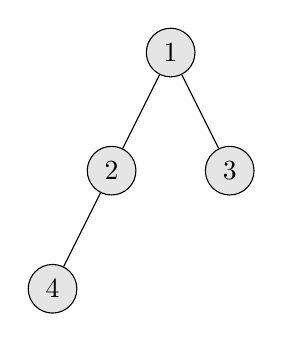
\begin{tikzpicture}
[every node/.style={draw, circle, fill=gray!20!, minimum size=5mm}]
\node{1}
child{node{2} child{node{4}} child[missing]}
child{node{3}};
\end{tikzpicture}
\end{figure}

\textbf{Output}: $ 1(2(4))(3) $

\textbf{Explanation}: 

Originally it needs to be $ 1(2(4)())(3()()) $, 

but you need to omit all the unnecessary empty parenthesis pairs. 

And it will be $ 1(2(4))(3) $.
\end{flushleft}

\paragraph{Example 2:}
\begin{flushleft}

\textbf{Input}:
\begin{figure}[H]
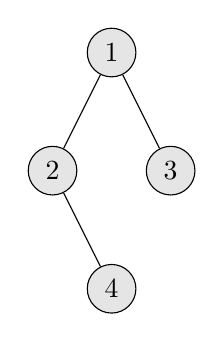
\begin{tikzpicture}
[every node/.style={draw, circle, fill=gray!20!, minimum size=5mm}]
\node{1}
child{node{2} child[missing] child{node{4}}}
child{node{3}};
\end{tikzpicture}
\end{figure}

\textbf{Output}: $ 1(2()(4))(3) $

\textbf{Explanation}: 

Almost the same as the first example, 

except we can't omit the first parenthesis pair to break the one-to-one mapping relationship between the input and the output.
\end{flushleft}
% \section{607 --- Sales Person}

SQL problem.
% \section{608 --- Tree Node}

SQL Problem.
% \section{609 --- Find Duplicate File in System}
Given a list of directory info including directory path, and all the files with contents in this directory, you need to find out all the groups of duplicate files in the file system in terms of their paths.

A group of duplicate files consists of at least two files that have exactly the same content.

A single directory info string in the input list has the following format:

\path{root/d1/d2/.../dm f1.txt(f1_content) f2.txt(f2_content) ... fn.txt(fn_content)}

It means there are $n$ files (\path{f1.txt}, \path{f2.txt}, \textellipsis, \path{fn.txt} with content f1\_content, f2\_content \textellipsis fn\_content, respectively) in directory \path{root/d1/d2/.../dm}. Note that $n \geq 1$ and $m \geq 0$. If $m = 0$, it means the directory is just the root directory.

The output is a list of group of duplicate file paths. For each group, it contains all the file paths of the files that have the same content. A file path is a string that has the following format:

\path{directory_path/file_name.txt}

\paragraph{Example 1:}

\textbf{Input}:

[\path{root/a} \path{1.txt}(abcd) \path{2.txt}(efgh), \path{root/c} \path{3.txt}(abcd), \path{root/c/d} \path{4.txt}(efgh), \path{root} \path{4.txt}(efgh)]

\textbf{Output}:
  
[[\path{root/a/2.txt}, \path{root/c/d/4.txt}, \path{root/4.txt}],[\path{root/a/1.txt}, \path{root/c/3.txt}]]

 

\paragraph{Note:}

\begin{itemize}
\item No order is required for the final output.
\item You may assume the directory name, file name and file content only has letters and digits, and the length of file content is in the range of $[1,50]$.
\item The number of files given is in the range of $[1,20000]$.
\item You may assume no files or directories share the same name in the same directory.
\item You may assume each given directory info represents a unique directory. Directory path and file info are separated by a single blank space.
\end{itemize}

 
\paragraph{Follow-up:}

\begin{itemize}
\item Imagine you are given a real file system, how will you search files? DFS or BFS?
\item If the file content is very large (GB level), how will you modify your solution?
\item If you can only read the file by 1kb each time, how will you modify your solution?
\item What is the time complexity of your modified solution? What is the most time-consuming part and memory consuming part of it? How to optimize?
\item How to make sure the duplicated files you find are not false positive?
\end{itemize}

\subsection{Hash Map}
\begin{itemize}
    \item Get directory, file name and content from the input strings.
    \item Group files per their contents.
\end{itemize}

\subsection{Follow Up Questions:}
\begin{enumerate}
    \item If depth of directory is not too deeper, which is suitable to use DFS, comparing with BFS.
    \item core idea: make use of meta data, like file size before really reading large content. 
    \begin{itemize}
        \item  DFS to map each size to a set of paths that have that size: Map<Integer, Set>
    \item For each size, if there are more than 2 files there, compute hashCode of every file by MD5, if any files with the same size have the same hash, then they are identical files: Map<String, Set>, mapping each hash to the Set of filepaths+filenames. 
    \end{itemize}
\end{enumerate}

% \section{610 --- Triangle Judgement}

SQL Problem.
\section{611 --- Valid Triangle Number}
Given an array consists of non-negative integers,  $A$, your task is to count the number of triplets chosen from the array that can make triangles if we take them as side lengths of a triangle.

\paragraph{Example 1:}

\begin{flushleft}
\item \textbf{Input}: $[2,2,3,4]$

\textbf{Output}: 3

\textbf{Explanation}:

Valid combinations are: 

$2,3,4$ (using the first 2)

$2,3,4$ (using the second 2)

$2,2,3$

\end{flushleft}

\paragraph{Note:}

\begin{itemize}
\item The length of the given array won't exceed 1000.
\item The integers in the given array are in the range of $[0, 1000]$.
\end{itemize}

\subsection{Two Pointers}
Sort given array, and then iterate the array from end to beginning.

for each index $i$, we check with two index $l$ and $r$ where $l=0$ and $r=i-1$ at start. 

If \fcj{nums[l]+nums[r] > nums[i]}, then from $(l, r, i)$, $(l+1,r,i)$, $\ldots$, $(r-1,r,i)$ are all valid triangle numbers. The count is therefore $r-1-l+1=r-l$, and decrement $r$.

Otherwise, we just increment $l$ to test next number.

\setcounter{lstlisting}{0}
\begin{lstlisting}[style=customc, caption={Two Pointers}]
int triangleNumber( vector<int>& nums )
{
    sort( nums.begin(), nums.end() );
    long len = ( long )( nums.size() );
    int ans = 0;
    for( long i = len - 1; i >= 2 ; --i )
    {
        auto l = 0;
        auto r = i - 1;
        while( l < r )
        {
            if( nums[l] + nums[r] > nums[i] )
            {
                //(l,r,i), (l+1,r,i), ...(r-1, r, i)
                //all can form triangle numbers
                //total is (r-1-l+1=r-l)
                ans += ( r - l );
                --r;
            }
            else
            {
                ++l;
            }
        }
    }
    return ans;
}
\end{lstlisting}

\paragraph{Similar Problems}
\begin{itemize}
\item \textbf{259. 3Sum Smaller}
\end{itemize}


%\section{612 --- Shortest Distance in a Plane}

SQL problem
%\section{613 --- Shortest Distance in a Line}

SQL Problem
%\section{614 --- Second Degree Follower}

SQL Problem
%\section{615 --- Average Salary: Departments VS Company}

SQL Problem
% \section{616 --- Add Bold Tag in String}
Given a string $s$ and a list of strings $D$, you need to add a closed pair of bold tag \texttt{<b>} and \texttt{</b>} to wrap the substrings in $s$ that exist in $D$. If two such substrings overlap, you need to wrap them together by only one pair of closed bold tag. Also, if two substrings wrapped by bold tags are consecutive, you need to combine them.

\paragraph{Example 1:}

\begin{flushleft}
\textbf{Input}:
 
$s$: \texttt{abcxyz123}, $D$: [\texttt{abc},\texttt{123}]

\textbf{Output}:

\path{<b>abc</b>xyz<b>123</b>}

\end{flushleft}

\paragraph{Example 2:}

\begin{flushleft}
\textbf{Input}:
 
$s$: \texttt{aaabbcc}, $D$: [\texttt{aaa}, \texttt{aab}, \texttt{bc}]

\textbf{Output}:

\path{<b>aaabbc</b>c}
\end{flushleft}

\paragraph{Note:}

\begin{itemize}
\item The given list of string $D$ won't contain duplicates, and its length won't exceed 100.
\item All the strings in input have length in range [1, 1000].
\end{itemize}

\subsection{Brute Force}
Check for all all occurrences of each word and mark the corresponding letters bold.

\begin{itemize}
\item Maintain a boolean array $B$, where $B[i]$ indicate if letter $S[i]$ is belongs to a word in the given dictionary.
\item Iterate over $S$, at index $i$, for each word, $W$, if $S[i]$ starts with $W$, then $B[i, i+\lvert W\rvert-1]$ will be set to 1.
\item With the filled $B$, the position to insert the start and end bold tags are known.
\begin{enumerate}
\item for the start boild tag, if $B[i]=1$ and $B[i-1]=0$, we will insert begin tag before $S[i]$. The edge case is $i=0$. If $B[0]=1$, we directly insert begin tag before $S[0]$.
\item for the end bold tag, if $B[i]=1$ and $B[i+1]=0$, we will insert end tag after $S[i]$. The edge case is $i=L-1$ where $L$ is the length of $s$. If $B[L-1]=1$, we directly insert end tag after $S[L-1]$.
\end{enumerate}
\end{itemize}


\subsection{Merge Interval}
\begin{itemize}
\item Find every index $i$ in $S$ such that $S[i]$ is starting with a word in the given dictionary, and record each starting and ending index as an interval.
\item Then we merge the intervals from previous step. 
\item Finally, we insert begin and end bold tag per each merged interval.
\end{itemize}


% \section{617 --- Merge Two Binary Trees}
Given two binary trees and imagine that when you put one of them to cover the other, some nodes of the two trees are overlapped while the others are not.

You need to merge them into a new binary tree. The merge rule is that if two nodes overlap, then sum node values up as the new value of the merged node. Otherwise, the NOT null node will be used as the node of new tree.

\paragraph{Example 1:}

\begin{flushleft}
\textbf{Input}:

\begin{figure}[H]
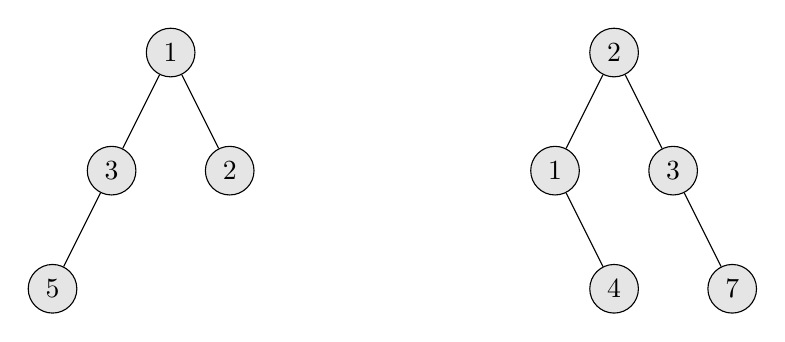
\begin{tikzpicture}
[every node/.style={draw, circle, fill=gray!20!, minimum size=5mm}]
\node(1){1}
child{node{3} child{node{5}} child[missing]}
child{node{2}};

\node[right= of 1, xshift=4cm ]{2}
child{node{1} child[missing] child{node{4}}}
child{node{3} child[missing] child{node{7}}};
\end{tikzpicture}
\end{figure}


\textbf{Output}:

\begin{figure}[H]
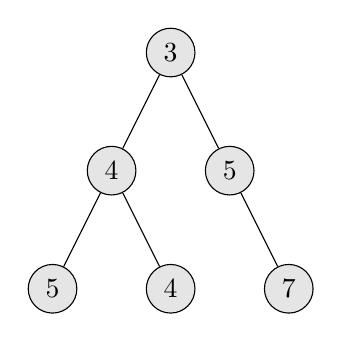
\begin{tikzpicture}
[every node/.style={draw, circle, fill=gray!20!, minimum size=5mm}]
\node{3}
child{node{4} child{node{5}} child{node{4}}}
child{node{5} child[missing] child{node{7}}};
\end{tikzpicture}
\end{figure}


\end{flushleft}

\paragraph{Note:} 
\begin{itemize}
\item The merging process must start from the root nodes of both trees.
\end{itemize}

\subsection{Recursion}
We can traverse both the given trees in a \textbf{preorder} fashion. 
\begin{itemize}
    \item At every step, we check if the current node is not null for both the trees. If so, we add the values in the current nodes of both the trees and update the value in the current node of the first tree to reflect this sum obtained. 
    \item At every step, we also call the original function with the left children and then with the right children of the current nodes of the two trees. If at any step, one of these children happens to be null, we return the child of the other tree(representing the corresponding child subtree) to be added as a child subtree to the calling parent node in the first tree. 
    \item At the end, the first tree will represent the required resultant merged binary tree.
\end{itemize}
%\section{618 --- Students Report By Geography}

SQL Problem
%\section{619 --- Biggest Single Number}

SQL Problem
%\section{620 --- Not Boring Movies}

SQL Problem
% \section{621 --- Task Scheduler}
Given a char array, $A$, representing tasks CPU need to do. It contains capital letters \texttt{A} to \texttt{Z} where different letters represent different tasks. Tasks could be done without original order. Each task could be done in one interval. For each interval, CPU could finish one task or just be idle.

However, there is a non-negative cooling interval $n$ that means between two same tasks, there must be at least $n$ intervals that CPU are doing different tasks or just be idle.

You need to return the least number of intervals the CPU will take to finish all the given tasks.
 

\paragraph{Example:}

\begin{flushleft}
\textbf{Input}: tasks: $[A, A, A, B, B, B]$, $n = 2$

\textbf{Output}: 8

\textbf{Explanation}: $A \longrightarrow B \longrightarrow \texttt{idle} \longrightarrow A \longrightarrow B \longrightarrow \texttt{idle} \longrightarrow A \longrightarrow B$.

\end{flushleft}
 

\paragraph{Note:}

\begin{itemize}
\item The number of tasks is in the range $[1, 10000]$.
\item The integer $n$ is in the range $[0, 100]$.

\end{itemize}


\subsection{Calculate Idle Slots}
\begin{itemize}
\item If we can get the number of idle slots $x$, the time required to execute all the tasks are $x+z$ where $z$ is the number of total tasks.
\item To find the idle time, take following figure as below ($n=5$):
\begin{figure}[H]
\centering
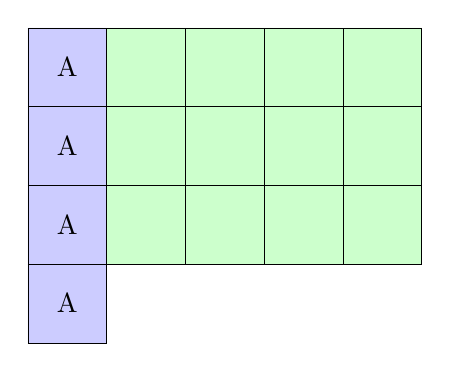
\begin{tikzpicture}
[thick]
\draw[help lines, draw=black, fill=blue!20!] (0,0) grid (1, 4) rectangle (0,0);
\draw[help lines, draw=black, fill=green!20!] (1,1) grid (5, 4) rectangle (1,1);
\node at (0.5, 0.5) {A};
\node at (0.5, 1.5) {A};
\node at (0.5, 2.5) {A};
\node at (0.5, 3.5) {A};
\end{tikzpicture}
\end{figure}
In the figure, the green part represents the idle slots. We can observe that the maximum number of idle slots will always be given by the product of the cooling time and the number of instances of the task with maximum count less 1(in case only multiple instances of the same task need to be executed, and each, then, is executed after lapse of every cooling time). 

The factor of 1 is deducted from the task's count with maximum number of instances, as is clear from the figure, is that in the last round of execution of the tasks, the idle slots need not be considered for insertion following the execution of the related task. 

Now, based on the count of the instances of the other tasks, we can reduce the number of idle slots from this maximum value, to determine the minimum number of idle slots needed.
\item To do that, check the following graph. Assuming the tasks are executed in row-wise order, we can see that in case the number of instances of another task equal the number of instances of the task with maximum number of instances, the number of idle slots saved is equal to its number of instances less 1 as is clear for the case of task B as below. 

\begin{figure}[H]
\centering
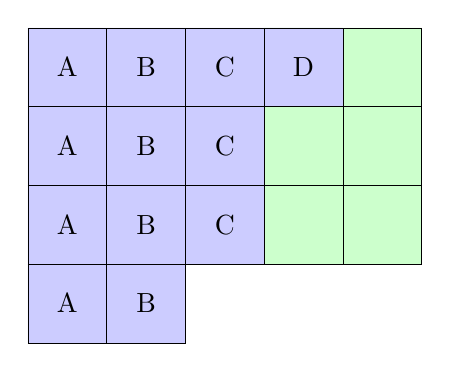
\begin{tikzpicture}
[thick]
\draw[help lines, draw=black, fill=blue!20!] (0,0) grid (1, 4) rectangle (0,0);
\draw[help lines, draw=black, fill=blue!20!] (1,0) grid (2, 4) rectangle (1,0);
\draw[help lines, draw=black, fill=blue!20!] (2,1) grid (3, 4) rectangle (2,1);
\draw[help lines, draw=black, fill=green!20!] (3,1) grid (5, 4) rectangle (3,1);
\node at (0.5, 0.5) {A};
\node at (0.5, 1.5) {A};
\node at (0.5, 2.5) {A};
\node at (0.5, 3.5) {A};

\node at (1.5, 0.5) {B};
\node at (1.5, 1.5) {B};
\node at (1.5, 2.5) {B};
\node at (1.5, 3.5) {B};

\node at (2.5, 1.5) {C};
\node at (2.5, 2.5) {C};
\node at (2.5, 3.5) {C};

\draw[help lines, draw = black, fill=blue!20!] (3,3) grid ++(1,1) rectangle (3,3);
\node at (3.5,3.5) {D};

\end{tikzpicture}
\end{figure}

But, if the count of the number of instances, say $i$ is less than the this maximum value, the number of idle slots saved is equal to the value $i$ itself as is clear for the case of task C. 

Further, for any arbitrary task other than A, B or C with the count of number of instances less than C, such as D. This task can be 
\begin{enumerate}
\item accommodated into the idle slots or 
\item if no more idle slot is available, this task can be appended after every row of tasks without interfering with the cooling time.
\end{enumerate}

In the first case, subtracting its number of instances from the number of idle slots leads to obtaining the correct number of available idle slots. 

In the second case, which will only occur if the number of idle slots pending is already zero, it leads to negative net idle slots, which can later be considered as zero for the purpose of calculations.
\end{itemize}


% \section{622 --- Design Circular Queue}
Design your implementation of the circular queue. The circular queue is a linear data structure in which the operations are performed based on FIFO (First In First Out) principle and the last position is connected back to the first position to make a circle. It is also called "Ring Buffer".

One of the benefits of the circular queue is that we can make use of the spaces in front of the queue. In a normal queue, once the queue becomes full, we cannot insert the next element even if there is a space in front of the queue. But using the circular queue, we can use the space to store new values.

Your implementation should support following operations:

\begin{lstlisting}[style=customc]
MyCircularQueue( k ); //Constructor, set the size of the queue to be k.

Front(); // Get the front item from the queue. If the queue is empty, return -1.

Rear(); //Get the last item from the queue. If the queue is empty, return -1.

enQueue( value ); //Insert an element into the circular queue. Return true if the operation is successful.

deQueue(); //Delete an element from the circular queue. Return true if the operation is successful.

isEmpty(); //Checks whether the circular queue is empty or not.

isFull(); //Checks whether the circular queue is full or not.
\end{lstlisting}

 

\paragraph{Example:}

\begin{lstlisting}[style=customc]
MyCircularQueue circularQueue = new MyCircularQueue( 3 ); // set the size to be 3
circularQueue.enQueue( 1 ); // return true
circularQueue.enQueue( 2 ); // return true
circularQueue.enQueue( 3 ); // return true
circularQueue.enQueue( 4 ); // return false, the queue is full
circularQueue.Rear();  // return 3
circularQueue.isFull();  // return true
circularQueue.deQueue();  // return true
circularQueue.enQueue( 4 ); // return true
circularQueue.Rear();  // return 4
\end{lstlisting}

 

\paragraph{Note:}

\begin{itemize}
\item  All values will be in the range of $[0, 1000]$.
\item The number of operations will be in the range of $[1, 1000]$.
\item Please do not use the built-in Queue library.
\end{itemize}

\subsection{Head and Tail Indexes}
\begin{itemize}
\item If the internal array is full utilized, we cannot differentiate between empty and full for a circular buffer because head is equal to tail in both cases.
\item One way to overcome this issue is to let the internal array has $k+1$ items where $k$ is the maximum capacity of the circular buffer. In this approach, when head is equal to tail, the buffer is empty. Instead, when tail is one less than head, the buffer is full.
\item Denote head and tail indexes are $x$ and $y$ respectively.
\begin{enumerate}
\item At start, $x=y=0$.
\item When push to the queue, first check if the queue is full. If not full, put the data at $y$ and then increments $y$ as $y\gets (y+1) \bmod L$. Here $L$ is the size of the internal vector which is one more than the capacity of the queue.
\item For dequeue operation, first check if the queue is empty. If not empty, increments the head index $x$ as $x\gets (x+1) \bmod L$.
\item To get the front of queue, simply returns element at head index $x$.
\item To get the rear of queue, since tail has incremented for each push operation, we need to get element at the index that is before the tail, i.e., $(x-1+L)\bmod(L)$.
\item If $x=y$, queue is empty.
\item If $(y+1)\bmod L = x$, queue is full.
\end{enumerate}
\end{itemize}

% \section{623 --- Add One Row to Tree}
Given the root of a binary tree, then value $v$ and depth $d$, you need to add a row of nodes with value $v$ at the given depth $d$. The root node is at depth 1.

The adding rule is: given a positive integer depth $d$, for each \textbf{NOT} null tree nodes $N$ in depth $d-1$, create two tree nodes with value $v$ as $N$'s left subtree root and right subtree root. And $N$'s \textbf{original left subtree} should be the left subtree of the new left subtree root, its \textbf{original right subtree} should be the right subtree of the new right subtree root. If depth $d$ is 1 that means there is no depth $d-1$ at all, then create a tree node with value $v$ as the new root of the whole original tree, and the original tree is the new root's left subtree.

\paragraph{Example 1:}
\begin{flushleft}
\textbf{Input:}

A binary tree as following:
\begin{figure}[H]
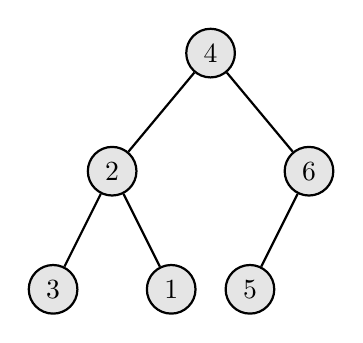
\begin{tikzpicture}
[every node/.style={draw, circle, fill=gray!20!, minimum size=5mm},
level 1/.style={sibling distance=25mm},
level 2/.style={sibling distance=15mm},
thick]
\node{4}
child{node{2} child{node{3}} child{node{1}}}
child{node{6} child{node{5}} child[missing]};
\end{tikzpicture}
\end{figure}

$v = 1$

$d = 2$

\textbf{Output}:
\begin{figure}[H]
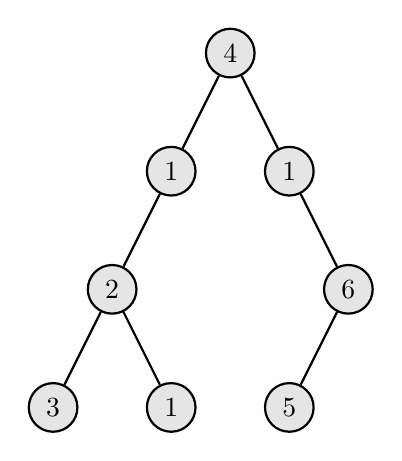
\begin{tikzpicture}
[every node/.style={draw, circle, fill=gray!20!, minimum size=5mm}, thick]
\node{4}
child{node{1} child{node{2} child{node{3}} child{node{1}} } child[missing]}
child{node{1} child[missing] child{node{6} child{node{5}} child[missing]}};
\end{tikzpicture}
\end{figure}

\end{flushleft}
 
%
\paragraph{Example 2:}

\begin{flushleft}

\textbf{Input}:
 
A binary tree as following:

\begin{figure}[H]
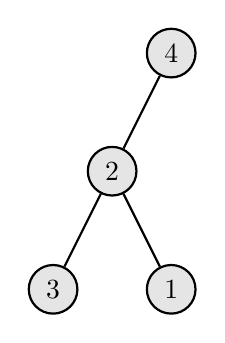
\begin{tikzpicture}
[every node/.style={draw, circle, fill=gray!20!, minimum size=5mm}, , thick]
\node{4}
child{node{2} child{node{3}} child{node{1}}}
child[missing];
\end{tikzpicture}
\end{figure}

$v = 1$

$d = 3$

\textbf{Output}:

\begin{figure}[H]
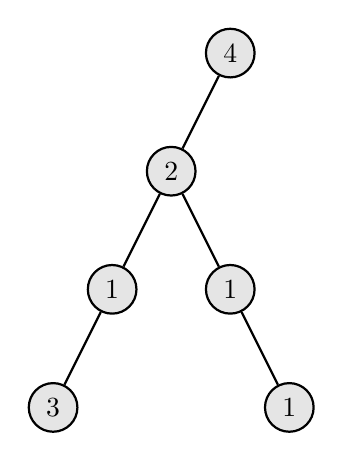
\begin{tikzpicture}
[every node/.style={draw, circle, fill=gray!20!, minimum size=5mm}, thick]
\node{4}
child{node{2} child{node{1} child{node{3}} child[missing]} child{node{1} child[missing] child{node{1}}}}
child[missing];
\end{tikzpicture}
\end{figure}

\end{flushleft}

\paragraph{Note:}

\begin{itemize}
\item The given $d$ is in range [1, maximum depth of the given tree $+ 1$].
\item The given binary tree has at least one tree node.
\end{itemize}

\subsection{DFS With Queue}
\begin{itemize}
\item We can iterate the tree level by level through a queue.
\item When reach depth $d-1$, make changes per the instruction.
\end{itemize}


% \section{624 --- Maximum Distance in Arrays}
Given $m$ arrays, and each array is sorted in ascending order. Now you can pick up two integers from two different arrays (each array picks one) and calculate the distance. We define the distance between two integers $a$ and $b$ to be their absolute difference $\lvert a-b\rvert$. Your task is to find the maximum distance.

\paragraph{Example 1:}

\begin{flushleft}
\textbf{Input}:

$\begin{bmatrix}
1 & 2 & 3\\
4 & 5 & \emptyset\\
1 & 2 & 3
\end{bmatrix}$

\textbf{Output}: 4

\textbf{Explanation}:
 
One way to reach the maximum distance 4 is to pick 1 in the first or third array and pick 5 in the second array.
\end{flushleft}

\paragraph{Note:}

\begin{itemize}
\item Each given array will have at least 1 number. There will be at least two non-empty arrays.
\item The total number of the integers in all the m arrays will be in the range of $[2, 10000]$.
\item The integers in the $m$ arrays will be in the range of $[-10000, 10000]$.
\end{itemize}

\subsection{Single Scan}
\begin{itemize}
\item If we consider two arrays: $A$ and $B$, we can just find the maximum out of $A[n−1]-B[0]$ and $B[m−1]-A[0]$ to find the larger distance. Here, $n$ and $m$ refer to the lengths of arrays $A$ and $B$ respectively. 

\item We keep a track of the element with minimum value, $x$, and the one with maximum value, $y$, found so far. Thus, now these extreme values can be treated as if they represent the extreme points of a cumulative array of all the arrays that have been considered until now.
\item For every new array, $T$, we find the distance $T[n−1] - x$ and $y-T[0]$ to compare with the maximum distance found so far. Here, $n$ refers to the number of elements in the current array, $T$. Note that the maximum distance found until now needs not always be contributed by the end points of the distance being maximum value, $y$, and minimum value, $x$.
\end{itemize}
% \section{625 --- Minimum Factorization}
Given a positive integer $a$, find the smallest positive integer $b$ whose multiplication of each digit equals to $a$.

If there is no answer or the answer is not fit in 32-bit signed integer, then return 0.

\paragraph{Example 1}

\begin{flushleft}
\textbf{Input}:

48 

\textbf{Output}:

68
\end{flushleft}

\paragraph{Example 2}
\begin{flushleft}
\textbf{Input}:

15

\textbf{Output}:

35
\end{flushleft}

\subsection{Factorization}
\begin{itemize}
    \item We know that the final number generated, $x$, should be such that its digits should have a product equal to the given number $a$. In other words, the digits of $x$ will be the factors of the given number $a$. Thus, our problem reduces to finding the factors(not necessarily prime) of $a$ and finding their smallest possible arrangement. 
    \item We start with trying with the largest possible factor $9$, obtain as many such counts of this factor as possible in $x$ and place such factors obtained at its least significant positions. Then, we go on decrementing the number currently considered as the possible factor and if it is a factor, we keep on placing it at relatively more significant positions in $x$. We go on getting such factors till we are done considering all the numbers from 9 to 2. \item At the end, $x$ gives the required result.
\end{itemize}
%\section{626 --- Exchange Seats}

SQL Problem
%\section{627 --- Swap Salary}

SQL Problem
% \section{628 --- Maximum Product of Three Numbers}
Given an integer array, $A$, find three numbers whose product is maximum and output the maximum product.

\paragraph{Example 1:}
\begin{flushleft}


\textbf{Input}: $[1,2,3]$

\textbf{Output}: 6
 
\end{flushleft}

\paragraph{Example 2:}

\begin{flushleft}
\textbf{Input}: $[1,2,3,4]$

\textbf{Output}: 24
\end{flushleft} 

\paragraph{Note:}
\begin{itemize}
    \item The length of the given array will be in range $[3,10^4]$ and all elements are in the range $[-1000, 1000]$.
    \item Multiplication of any three numbers in the input won't exceed the range of 32-bit signed integer.
\end{itemize}

\subsection{Single Scan}
\begin{itemize}
    \item To deal with negative and positive values, we require to find 2 smallest values, $x$ and $y$ ($x\leq y$), and the three largest values, $s$, $t$ and $u$ ($s\leq t\leq u$) in the give array $A$, by iterating over $A$ array only once.
    \item At the end, again we can find out the larger value out of $x\times y \times u$ and $s\times t\times u$ to find the required maximum product.
\end{itemize}
% \section{629 --- K Inverse Pairs Array}
Given two integers $n$ and $k$, find how many different arrays consist of numbers from 1 to $n$ such that there are exactly $k$ inverse pairs.

We define an inverse pair as following: For $i$th and $j$th element in the array, if $i < j$ and $a[i] > a[j]$ then it's an inverse pair; Otherwise, it's not.

Since the answer may be very large, the answer should be modulo $10^9 + 7$.

\paragraph{Example 1:}
\begin{flushleft}

\textbf{Input}: $n = 3$, $k = 0$

\textbf{Output}: 1

Explanation: 

Only the array $[1,2,3]$ which consists of numbers from 1 to 3 has exactly 0 inverse pair.


\end{flushleft} 

\paragraph{Example 2:}

\begin{flushleft}

\textbf{Input}: $n = 3$, $k = 1$

\textbf{Output}: 2

\textbf{Explanation}: 

The array $[1,3,2]$ and $[2,1,3]$ have exactly 1 inverse pair.

\end{flushleft} 

\paragraph{Note:}

\begin{itemize}
\item The integer $n$ is in the range $[1, 1000]$ and $k$ is in the range $[0, 1000]$.
\end{itemize}
\subsection{Dynamic Programming With 2D Array}


\begin{itemize}
\item Suppose $A=​ [2,4,1,3]$ which has $k=3$ inverse pairs ( $(2,1)$, $(4,1)$ and $(4,3)$). If a new number 5 is added to the end of $A$, the new array , say, $B$, is $[2,4,1,3,5]$. Because 5 is added at the end, it doesn't add any new inverse pair to the total number of inverse pairs from $A_1$.
\item Similarly, if we add 5 at $y$ position from the right end of $A$, then $y$ numbers smaller than 5 will be right to 5. Thus, this adds a total of $y$ inverse pairs to the total counts of inverse pairs in $A$. So, $B$ will have $3+y$ inverse pairs.

\item From the above example, if we know the number of inverse pairs, say $z$, in an array with elements from 1 to $n$, We can add a new element $n+1$ to this array at $p$ position from the right end. The total inverse pairs for the new generated array will be $z+p$.

\item In all, to generate the arrangements with exactly $k$ inverse pairs and $n$ elements, we can 

\begin{itemize}
\item Add the new number $n$ at the end of array with elements from 1 to $n-1$ and $k$ inverse pairs. 
\item Add $n$ at a position 1 step from the right end of array with elements from 1 to $n-1$ and $k-1$ inverse pairs.
\item $\ldots$
\item Add $n$ at a position $i$ steps from the right end of array with elements from 1 to $n-1$ and $k-i$ inverse pairs.
\end{itemize}
\item The above recursive relationship suggests a dynamic programming approach. Suppose $F(x,y)$ represents the number of arrangements with $x$ elements (from 1 to $x$) and exactly $y$ inverse pairs.

\begin{enumerate}
\item If $x=0$, no inverse pairs exist. Thus, $F(0, y)=0$.

\item If $y=0$, only one arrangement is possible, which is all numbers sorted in ascending order. Thus, $F(x,0)=1$.

\item Otherwise, $F(x,y)=\sum\limits_{i=0}^{\min(y, x-1)}F(x−1,y−i)$.
\end{enumerate}

Note that the upper limit on the summation is $\min(y,x−1)$. This is because for $i>y$, $y−i<0$. No arrangement exists with negative number of inverse pairs. The reason for the other factor can be seen as follows.

\item Next, we can simplify the above recursion formula:

\[F(x,y) = F(x-1,y) + F(x-1, y-1) + \ldots + F(x-1, y-i) + \ldots + F(x-1, y-(x-1))\]

Then 

\begin{align*}
F(x,y+1) &= F(x-1, y+1) + F(x-1, y) + \ldots \\
&+ F(x-1, y+1-i) + F(x-1, y-i) + \ldots + F(x-1, y+1-(x-1)) \\
  &= F(x-1, y+1) + F(x, y) - F(x-1, y-(x-1)) 
\end{align*}

replace $y+1$ by $y$ again in the above equation, we got

\[ F(x,y) = F(x, y-1) + F(x-1, y) - F(x-1, y-x) \]

The last item $F(x-1, y-x)$ only works for $y \geq x$.

\item Finally, $F(n, k)$ gives the result.
\end{itemize}

\subsection{Dynamic Programming With 1-D Array}
By observing the recursive formula:
\[ F(x,y) = F(x, y-1) + F(x-1, y) - F(x-1, y-x) \]
we can find that $F(x,y)$ only depends on previous row. Therefore, we can change the 2-D array to 1-D array. In this approach, $F$ contains all the results of one row, so $F$ size is $k+1$. 

In each iteration, we save $F$ to a temporary array $T$, i.e., $T$ contains all the results of previous row. Then, we update $F$ as $F(y)\gets F(y-1) + T(y) - T(y-1)$ for $1\leq y\leq n$ and $F(0)=1$.

% \section{630 --- Course Schedule III}
There are $n$ different online courses numbered from 1 to $n$. Each course has some duration (course length) $t$ and closed on $d$-th day. A course should be taken continuously for $t$ days and must be finished before or on the $d$-th day. You will start at the 1st day.

Given $n$ online courses represented by pairs $(t,d)$, your task is to find the maximal number of courses that can be taken.

\paragraph{Example:}
\begin{flushleft}

\textbf{Input}: $[[100, 200], [200, 1300], [1000, 1250], [2000, 3200]]$

\textbf{Output}: 3

\textbf{Explanation}: 

There are totally 4 courses, but you can take 3 courses at most:

First, take the 1st course, it costs 100 days so you will finish it on the 100th day, and ready to take the next course on the 101st day.

Second, take the 3rd course, it costs 1000 days so you will finish it on the 1100th day, and ready to take the next course on the 1101st day. 

Third, take the 2nd course, it costs 200 days so you will finish it on the 1300th day.
 
The 4th course cannot be taken now, since you will finish it on the 3300th day, which exceeds the closed date.

\end{flushleft}

\paragraph{Note:}

\begin{itemize}
\item The integer $1 \leq d, t, n \leq 10000$.
\item You can't take two courses simultaneously.
\end{itemize}

\subsection{Greedy}
\begin{itemize}
\item Sort the input per the end time of the course.
\item Maintain a variable $t$ to indicate current start time.
\item Go over the sorted array, if current course $c$ can be taken, i.e. $t + d_c \leq e_c$ ($d_c$ is the duration of course $c$ and $e_c$ is the day that $c$ has to be finished). We add $c$'s duration into a maximum priority queue (i.e., the top of the queue is the maximum one). 
\item If current course $c$ cannot be taken, we need to replace the largest duration from the priority queue with current course. At the same time, we have adjust start time $t$ by subtracting the largest duration from the queue because we don't take this lesson and adding $c$'s duration to $t$. Also, we need to push $c$'s duration into the queue.
\item Finally, the number of items in the queue gives us the answer.
\end{itemize}
% \section{631 --- Design Excel Sum Formula}
Your task is to design the basic function of Excel and implement the function of sum formula. Specifically, you need to implement the following functions:

\begin{lstlisting}[style=customc]
/**
Excel(int H, char W):

This is the constructor.
The inputs represents the height and width of the Excel form.
H is a positive integer, range from 1 to 26.
It represents the height.

W is a character range from 'A' to 'Z'.
It represents that the width is the number of characters from 'A' to W.

The Excel form content is represented by a height * width 2D integer array C,
it should be initialized to zero.
You should assume that the first row of C starts from 1,
and the first column of C starts from 'A'.
**/

Excel( int H, char W );

/**
void Set(int row, char column, int val): Change the value at C(row, column) to be val.
**/

void Set( int row, char column, int val );

/**
int Get(int row, char column): Return the value at C(row, column).
**/

int Get( int row, char column );

/**
int Sum(int row, char column, List of Strings : numbers):

This function calculate and set the value at C(row, column),
where the value should be the sum of cells represented by numbers.
This function return the sum result at C(row, column).
This sum formula should exist until this cell is overlapped
by another value or another sum formula.

numbers is a list of strings that each string represent a cell or a range of cells.
If the string represent a single cell, then it has the following format : ColRow.
For example, "F7" represents the cell at (7, F).
**/
int Sum( int row, char column, List of Strings : numbers );
\end{lstlisting}



\paragraph{Example 1:}

\begin{lstlisting}[style=customc]
/**
 construct a 3*3 2D array with all zero.

   A B C
 1 0 0 0
 2 0 0 0
 3 0 0 0
**/
Excel( 3, "C" );

/**
 set C(1,"A") to be 2.

   A B C
 1 2 0 0
 2 0 0 0
 3 0 0 0
**/
Set( 1, "A", 2 );

/**
 set C(3,"C") to be the sum of value at C(1,"A") and
 the values sum of the rectangle range
 whose top-left cell is C(1,"A") and bottom-right cell is C(2,"B").

 Return 4.

   A B C
 1 2 0 0
 2 0 0 0
 3 0 0 4
**/
Sum( 3, "C", ["A1", "A1:B2"] );

/**

set C(2,"B") to be 2. Note C(3, "C") should also be changed.

   A B C
 1 2 0 0
 2 0 2 0
 3 0 0 6
**/
Set( 2, "B", 2 );
\end{lstlisting}

\paragraph{Note:}

\begin{itemize}
\item You could assume that there won't be any circular sum reference. For example, \texttt{A1 = sum(B1)} and \texttt{B1 = sum(A1)}.
\item The test cases are using double-quotes to represent a character.
\item Please remember to RESET your class variables declared in class Excel, as static/class variables are persisted across multiple test cases. Please see here for more details.
\end{itemize}

\subsection{Topological Sort}
When we make any change to any cell, $x$, we need to determine the cells which are dependent on $x$, and update these cells, and further determine the cells which are dependent on the changed cells and so on. Since no cycles are present in the formulas, i.e. Any cell's value won't directly or indirectly be dependent on its own value.

Also, suppose cell $y$ is dependent on $x$. We need to update $x$  prior to $y$.

In order to do so, we can view the dependence between the cells in the form of a dependency graph, which can be a Directed Graph. Since no cycles are allowed between the formulas, the graph reduces to a Directed Acyclic Graph. Now, to solve the problem of evaluating the cells in the required order, we can make use of a very well known method specifically used for such problems in Directed Acyclic Graphs, known as the \textbf{Topological Sorting}.

Topological sorting for Directed Acyclic Graph (DAG) is a linear ordering of vertices such that for every directed edge $(u,v)$, vertex $u$ comes before $v$ in the ordering. For example, a topological sorting of the following graph is \textcolor{red}{5 4 2 3 1 0}.

\begin{figure}[H]
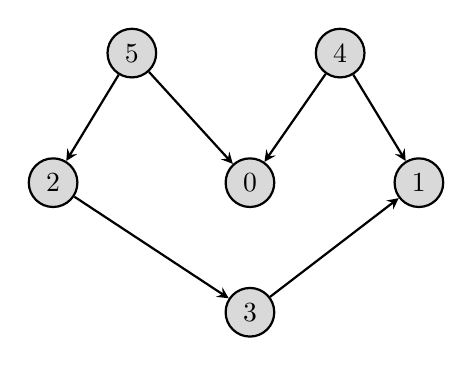
\begin{tikzpicture}
[every node/.style={draw, circle, fill=gray!30!, minimum size=5mm},
>=stealth, ->, thick]
\node(5) {5};
\node(4)[right=20mm of 5]{4};
\node(2)[below=10mm of 5, xshift=-10mm]{2};
\node(0)[below=10mm of 5, xshift=15mm]{0};
\node(1)[below=10mm of 4, xshift=10mm]{1};
\node(3)[below=10mm of 0]{3};
\draw (5) -- (2);
\draw (5) -- (0);
\draw (4) -- (0);
\draw (4) -- (1);
\draw (2) -- (3);
\draw (3) -- (1);
\end{tikzpicture}
\end{figure}

There can be more than one topological sorting for a graph. For example, another topological sorting of the following graph is \textcolor{red}{4 5 2 3 1 0}. The first vertex in topological sorting is always a vertex with in-degree as 0 (a vertex with no in-coming edges).

Topological Sorting can be done if we modify the Depth First Search to some extent. In Depth First Search, we start from a vertex, we first print it and then recursively call DFS for its adjacent vertices. Thus, the DFS obtained for the graph above, starting from node 5, will be \textcolor{red}{5 2 3 1 0 4}. But, in the case of a topological sort, we can't print a node until all the nodes on which it is dependent have already been printed.

To solve this problem, we make use of a temporary stack. We do the traversals in the same manner as in DFS, but we don’t print the current node immediately. Instead, for the current node we do as follows:

\begin{enumerate}
\item Recursively call topological sorting for all the nodes adjacent to the current node.

\item Push the current node onto a stack.

\item Repeat the above process till all the nodes have been considered at least once.

\item Print the contents of the stack.

\end{enumerate}

Note that a vertex is pushed to stack only when all of its adjacent(dependent) vertices (and their adjacent(dependent) vertices and so on) are already in stack. Thus, we obtain the correct ordering of the vertices. 

\subsection{Algorithm Implementation}
\begin{itemize}
\item For each cell, put all the other cells on which the cell's value is dependent into a hash map $M$. Therefore, each cell will have its associated hash map to store the cells that can affect its value.
\item The key of $M$ is the cell name, which is composed by the column letter and row number. The value of $M$ is the count of the cell happen in the sum formula. For example, $C1=C2+C3+C2$. In this case, the count of $C3$ is 1 and that of $C2$ is 2.
\item In function \texttt{set}, we need to clear the hash map of the cell at given $r$ and $c$, and then do the topological sorting to put the cells into a stack. Then, pop each cell from the stack, and set the sum of the values from its related cells as the value of this cell.
\item In function \texttt{sum}, we also clear the hash map of the cell at given $r$ and $c$, and then put all the cells from the formula into the map. Next, summation all the values from the cells in the map. Since this cell's value is changed, we also need to do topological sorting again to set the values of all the cells that depend on this cell at given $r$ and $c$.
\
\end{itemize}
% \section{632 --- Smallest Range}
You have $k$ lists of sorted integers in ascending order. Find the \textbf{smallest} range that includes at least one number from each of the $k$ lists.

We define the range $[a,b]$ is smaller than range $[c,d]$ if $b-a < d-c$ or $a < c$ if $b-a = d-c$.

\paragraph{Example 1:}

\begin{flushleft}
\textbf{Input}:$[[4,10,15,24,26], [0,9,12,20], [5,18,22,30]]$

\textbf{Output}: $[20,24]$

\textbf{Explanation}: 

List 1: $[4, 10, 15, 24,26]$, 24 is in range $[20,24]$.

List 2: $[0, 9, 12, 20]$, 20 is in range $[20,24]$.

List 3: $[5, 18, 22, 30]$, 22 is in range $[20,24]$.
\end{flushleft}

\paragraph{Note:}

\begin{itemize}
\item The given list may contain duplicates, so ascending order means $\geq$ here.
\item $ 1 \leq k \leq 3500$
\item $-10^5 \leq n \leq 10^5$, where $n$ is the value of element
\end{itemize}

\subsection{Brute Force}
The naive way is to compare each pair of elements, say $p_1 = A[x][i]$ and $ p_2 = A[y][j]$ from the given list. For each range, $R=[p_1, p_2]$, we can traverse the given list to find if at least one element in each list is contained in $R$. If so, compare with the minimum range so far and update it then.

But we can do better because all the arrays in the given list are sorted. Thus, we can make use of binary search to find if current range $R$ can contain at least one element of current array considered without testing each element in the array.

\setcounter{lstlisting}{0}
\begin{lstlisting}[style=customc, caption={Brute Force With Binary Search}]
vector<int> smallestRange( vector<vector<int>>& nums )
{

    int min_beg = -100000;
    int max_end = 100000;

    for( size_t x = 0; x < nums.size(); ++x )
    {
        for( size_t i = 0; i < nums[x].size(); ++i )
        {
            //p1=nums[x][i]

            for( size_t y = x; y < nums.size(); ++y )
            {
                //the range start and end
                //can both from same array
                for( size_t j = ( x == y ) ? i : 0; j < nums[y].size(); ++j )
                {
                    //get min and max of nums[x][i] and nums[y][j]
                    int beg = nums[x][i];
                    int end = nums[y][j];

                    if( beg > end )
                    {
                        swap( beg, end );
                    }

                    //test each array in nums
                    //to find if at least one element of each array
                    //can be contained in this range

                    bool flag = true;
                    for( const auto& arr : nums )
                    {
                        auto z = leftmost( arr, beg );

                        if( ( z == arr.size() ) || ( arr[z] > end ) )
                        {
                            //either arr.back() < beg or arr[0] > end
                            flag = false;
                            break;
                        }
                    }

                    if( flag )
                    {
                        //compare with global minimum range
                        if( ( end - beg < max_end - min_beg ) || ( ( end - beg == max_end - min_beg ) && ( min_beg > beg ) ) )
                        {
                            min_beg = beg;
                            max_end = end;
                        }
                    }

                } //end for j
            } //end for y

        } //end for i
    }// end for x

    return {min_beg, max_end};


}

size_t leftmost( const vector<int>& A, int target )
{
    size_t l = 0;
    size_t r = A.size();

    while( l < r )
    {
        auto mid = ( l + r ) / 2;
        if( A[mid] < target )
        {
            l = mid + 1;
        }
        else
        {
            r = mid;
        }
    }

    return l;
}
\end{lstlisting}

\subsection{Index Arrays}
In this approach, we maintain an array of indexes $I$ to track each array in the given list. The length of $I$ is equal to the one of the given list.

At start, all the entries in $I$ are zero. This means we are dealing with each array's minimum number. From these numbers, we get the maximum and minimum one, say $x$ and $y$, and the index of the lists that contains them, say $i$ and $j$. Apparently, range $R=[x,y]$ contains at least one number from each array in the given list. 

From now on, we try to minimize $R$ as much as possible. To do that, we can either increase $x$ or decrease $y$. Since $y$ is already a minimum number in one of array. If we decrease $y$ further, the range will include none of elements in that array. Thus, what we can do is increasing $x$.

Hence, we go to the array which contain $x$ and increment the index $t$ for this array to consider next number. Now, we have to update current minimum and maximum number because by advancing in one array may change these two values. We also need to record the indexes of the arrays that contain the current minimum and maximum number, and compare/update the global minimum range so far.
Whenever the index of an array reaches the end, we know that we cannot find any range that can contain at least one element from each array, the process is stopped.

Summarizing the statements above, the process becomes:

\begin{enumerate}
\item Initialize index array $T$ with all 0's.

\item Find the indices of the arrays containing the current minimum and the maximum elements among the elements by the indices in $T$.

\item If the range formed by the maximum and minimum elements found above is smaller than the global minimum range, update it.

\item Increment the index for the array that contains current minimum element.

\item   Repeat steps 2 to 4 untill any of the lists gets exhausted.

\end{enumerate}

\begin{lstlisting}[style=customc, caption={Index Array}]
vector<int> smallestRange( vector<vector<int>>& nums )
{
    //global range's start and end
    int min_beg = -100001;
    int max_end = 100001;

    //the array contains index for each array
    vector<size_t> T( nums.size(), 0 );

    //the index of array contains the current minimum element

    size_t min_ai = 0;

    while( true )
    {
        int x = 100001;
        int y = -100001;

        //we need to get current max and min element
        //not global
        for( size_t i = 0; i < nums.size(); ++i )
        {
            int n = nums[i][T[i]];

            if( n < x )
            {
                x = n;
                //the index of array contains minimum number
                min_ai = i;
            }

            if( n > y )
            {
                y = n;
            }

        }

        int min_range = max_end - min_beg;
        int cur_range = y - x;

        if( ( min_range > cur_range ) || ( ( min_range == cur_range ) && ( min_beg > x ) ) )
        {
            max_end = y;
            min_beg = x;
        }

        //go to the next element in the array
        //which contains the current min element
        ++T[min_ai];

        if( T[min_ai] == nums[min_ai].size() )
        {
            //we have already exhausted one of array
            //break now
            break;
        }

    }

    return {min_beg, max_end};
}
\end{lstlisting}
  
\subsection{Priority Queue}
The idea behind is similar to sort $K$ lists. In the last approach, we update the index in the array that containing current minimum element and traverse over $T$ array to determine the next maximum and minimum elements. By comparing the two steps in the last approach, almost all elements that are used to determine current maximum and minimum values are the same except the new element in the array that containing the minimum value in the last step. This new element could contribute to current maximum element. 

Thus, we actually find minimum element at every step. To avoid iterate the whole $T$ array, we can make use of min-heap which stores all the numbers at the indices from $T$ for each array. Since the heap has the minimum number at the top, we don't need to iterate over $T$ again to find new minimum element.

Thus, at each step, we remove the top which is the current minimum, and update current maximum by the next number in the array containing the current minimum. Form the range with this minimum and current maximum to compare and update global range. Then we add the new number in the array that containing current minimum element to the queue. Repeat the steps until one of array is exhausted.

\begin{lstlisting}[style=customc, caption={Priority Queue}]
vector<int> smallestRange( vector<vector<int>>& nums )
{
    using node_t = array<size_t, 2>;

    auto cmp = [&nums]( const node_t& n1, const node_t& n2 )
    {
        auto& A1 = nums[n1[0]];
        auto& A2 = nums[n2[0]];

        return A1[n1[1]] > A2[n2[1]];
    };

    priority_queue<node_t, vector<node_t>, decltype( cmp )> q( cmp );

    //current maximum
    int y = -100001;

    //the global minimum range
    //start and end
    int start = -100001;
    int end = 100001;

    //firstly, add first number of each array
    //into the queue
    for( size_t i = 0; i < nums.size(); ++i )
    {
        q.push( node_t{ i, 0 } );
        y = ( max )( y, nums[i][0] );
    }


    while( !q.empty() )
    {
        //remove the top
        auto t = q.top();
        q.pop();

        //the top is the global minimum
        //A is the array containing
        //the minimum element
        auto& A = nums[t[0]];

        int min_range = end - start;
        int cur_range = y - A[t[1]];

        if( ( cur_range < min_range ) || ( ( cur_range == min_range ) && ( A[t[1]] < start ) ) )
        {
            start = A[t[1]];
            end = y;
        }

        //go to the next element
        //int A
        auto next = t[1] + 1;

        if( next == A.size() )
        {
            break;
        }

        y = ( max )( A[next], y );

        q.push( node_t{t[0], next} );
    }

    return {start, end};
}
\end{lstlisting}
% \section{633 --- Sum of Square Numbers}
Given a non-negative integer $c$, your task is to decide whether there are two integers $a$ and $b$ such that $a^2 + b^2 = c$.

\paragraph{Example 1:}

\begin{flushleft}
\textbf{Input}: 5

\textbf{Output} True

\textbf{Explanation}: $1 \times 1 + 2 \times 2 = 5$

\end{flushleft}
 

\paragraph{Example 2:}

\begin{flushleft}
\textbf{Input}: 3

\textbf{Output}: False

\end{flushleft}

\subsection{Try From Both Ends}
$a$ and $b$ must be in the range $[0, \sqrt{c}]$. Thus, we can suppose $a\leq b$ and
\begin{enumerate}
\item test $a$ from 0 to $\sqrt{c}$
\item and test $b$ from $\sqrt{c}$ down to zero
\end{enumerate}

Then we repeat the following process

\begin{itemize}
\item $a^2+b^2=c$: we just directly return \texttt{True}. 

\item $a^2+b^2<c$: increments $a$.

\item $a^2+b^2>c$: decrements $b$.

\end{itemize}
The above process will end when $a > b$.

We also need to take care of data type overflow. We may need to use \texttt{long long} type during whole computation.


\subsection{Fermat Theorem}

This approach is based on the following statement, which is based on Fermat's Theorem:

\begin{quote}
    Any positive number $n$ is expressible as a sum of two squares if and only if the prime factorization of $n$, every prime of the form $(4k+3)$ occurs an even number of times.

\end{quote}

By making use of the above theorem, we find all the prime factors of the given number $c$, which could range from $[2,\sqrt{c}]$ along with the count of those factors, by repeated division. 

If at any step, we find out that the counts of any prime factor of the form $(4k+3)$ occurs an odd number of times, we can return a \texttt{False} value.

If $c$ itself is a prime number, it won't be divisible by any of the primes in the $[2,\sqrt{c}]$. Thus, we need to check if $c$ can be expressed in the form of $4k+3$. If so, we need to return a \texttt{False} value, indicating that this prime occurs an odd number(1) of times.

Otherwise, we can return a \texttt{True} value.

% \section{634 --- Find the Derangement of An Array}
In combinatorial mathematics, a derangement is a permutation of the elements of a set, such that no element appears in its original position.

There's originally an array consisting of $n$ integers from 1 to $n$ in ascending order, you need to find the number of derangement it can generate.

Also, since the answer may be very large, you should return the output mod $10^9 + 7$.

\paragraph{Example 1:}

\begin{flushleft}
Input: 3

Output: 2

Explanation: The original array is $ [1,2,3] $. The two derangements are $[2,3,1]$ and $[3,1,2]$.
\end{flushleft}
\paragraph{Note:}
\begin{itemize}
\item $n$ is in the range of $[1, 10^6]$. 
\end{itemize}

\subsection{Dynamic Programming}
Suppose the original array is $[1,2,\ldots, n]$. At first, we move the first number 1 to another index, say $p$. We have $n-1$ ways to choose $p$, i.e. from $1$ to $n-1$. Since number $p$ at index $p$ is replaced by 1, we have to find another index to place it. We have two options:

\begin{enumerate}
\item We place $p$ at the index of $1$, i.e, at index 0. Thus, the problem reduces to find the derangements of remaining $n-2$ numbers. The reason is, $p$ and $1$ are fixed, and we are left with $n-2$ indices to place $n-2$ numbers, and each number $i$ cannot be placed at index $i-1$.
\item We don't place $p$ at the index of $1$. In this case, the problem reduces to find the derangements of $n-1$ numbers. The reason is only $1$ is fixed, and we are left with $n-1$ indices to place $n-1$ numbers, and each number $i$ cannot be placed at index $i-1$.
\end{enumerate} 

Thus, let $F(n)$ is the number of derangements for array $[1,2,\ldots, n]$. Based on above analysis, we have:
\[
F(n) = (n-1)\times(F(n-1)+F(n-2))
\]
% \section{635 --- Design Log Storage System}
You are given several logs that each log contains a unique id and timestamp. Timestamp is a string that has the following format: Year:Month:Day:Hour:Minute:Second, for example, 2017:01:01:23:59:59. All domains are zero-padded decimal numbers.

Design a log storage system to implement the following functions:

\begin{itemize}
\item \lstinline[language=Java, basicstyle=\small\ttfamily, keywordstyle=\bfseries\color{green!40!black}]|void Put(int id, string timestamp)|: Given a log's unique id and timestamp, store the log in your storage system.

\item \lstinline[language=Java, basicstyle=\small\ttfamily, keywordstyle=\bfseries\color{green!40!black}]|int[] Retrieve(String start, String end, String granularity)|: Return the id of logs whose timestamps are within the range from \texttt{start} to \texttt{end}. \texttt{Start} and \texttt{end} all have the same format as timestamp. However, granularity means the time level for consideration. For example, \texttt{start}: \textcolor{red}{2017:01:01:23:59:59}, \texttt{end}: \textcolor{red}{2017:01:02:23:59:59}, \texttt{granularity}: \textcolor{red}{Day}, it means that we need to find the logs within the range from Jan. 1st 2017 to Jan. 2nd 2017.
\end{itemize}

\paragraph{Example 1:}

\begin{lstlisting}[style=customc]
put( 1, "2017:01:01:23:59:59" );
put( 2, "2017:01:01:22:59:59" );
put( 3, "2016:01:01:00:00:00" );

// return [1,2,3], because you need to return all
// logs within 2016 and 2017.
retrieve( "2016:01:01:01:01:01", "2017:01:01:23:00:00", "Year" );


// return [1,2], because you need to return all logs
// start from 2016:01:01:01 to 2017:01:01:23,
// where log 3 is left outside the range.
retrieve( "2016:01:01:01:01:01", "2017:01:01:23:00:00", "Hour" );
\end{lstlisting}


\paragraph{Note:}

\begin{itemize}
\item There will be at most 300 operations of \texttt{Put} or \texttt{Retrieve}.
\item Year ranges from $[2000,2017]$. Hour ranges from $[00,23]$.
\item Output for Retrieve has no order required.
\end{itemize}

\subsection{Transform}
\begin{itemize}
\item Since the year is in $[2000,2017]$, we can use 1999 as the base to transform the input timestamp into seconds from 1999.
\item Use a tree map as the underlying data structure because it can automatically sort the logs per their timestamps (seconds).
\item In order to retrieve the logs' ids lying within the given timestamp ranges, $s$ and $e$, and a granularity $g$. firstly, we need to convert the given timestamps into seconds. Before doing the conversion, we need to consider the effect of granularity.
 \begin{enumerate}
\item Granularity defines the precision of the results. For example, for a granularity corresponding to a \texttt{Day}, we only need to consider the portion of the timestamp up to \texttt{Day} section only. The rest of the fields can be assumed to be all zeros. 
\item After doing this for both the start and end timestamp, we do the conversion of the timestamp with the required precision into seconds. Once this has been done, we can use binary search to find the first item that is no less than the start and the last item that is no larger than the end.
\item There is a trick: to convert end timestamp to seconds, we can increment the value in the position of specified granularity. Therefore, we are looking for a half open range when doing the search.
\end{enumerate}
\end{itemize}
% \section{636 --- Exclusive Time of Functions}
On a single threaded CPU, we execute some functions.  Each function has a unique id between 0 and $N-1$.

We store logs in timestamp order that describe when a function is entered or exited.

Each log is a string with this format: \lstinline[language=Java, basicstyle=\small\ttfamily, keywordstyle=\bfseries\color{green!40!black}]|{function_id}:{["start","end"]}:{timestamp}|.  

For example, \texttt{0:start:3} means the function with id 0 started at the beginning of timestamp 3.  \texttt{1:end:2} means the function with id 1 ended at the end of timestamp 2.

A function's exclusive time is the number of units of time spent in this function.  Note that this does not include any recursive calls to child functions.

The CPU is single threaded which means that only one function is being executed at a given time unit.

Return the exclusive time of each function, sorted by their function id.
 

\paragraph{Example 1:}

\begin{flushleft}
\textbf{Input}: $n = 2$, \texttt{logs}: [\texttt{0:start:0}, \texttt{1:start:2}, \texttt{1:end:5}, \texttt{0:end:6}]

\textbf{Output}: $[3, 4]$

\textbf{Explanation}:

Function 0 starts at the beginning of time 0, then it executes 2 units of time and reaches the end of time 1.

Now function 1 starts at the beginning of time 2, executes 4 units of time and ends at time 5.

Function 0 is running again at the beginning of time 6, and also ends at the end of time 6, thus executing for 1 unit of time. 

So function 0 spends $2 + 1 = 3$ units of total time executing, and function 1 spends 4 units of total time executing.


\end{flushleft} 

\paragraph{Note:}

\begin{itemize}
\item $1 \leq n \leq 100$
\item Two functions won't start or end at the same time.
\item Functions will always log when they exit.
\end{itemize}

\subsection{Stack}
First, we need to understand the meaning of this problem:

\begin{itemize}
\item We are given a list of string, $A$, which depict how $n$ functions are executed in a single thread CPU.
\item A function $f_1$ could call function $f_2$, and $f_2$ may call another function $f_3$. As a result, $f_1$ starts first and end third, $f_2$ starts second and end second, and $f_3$ starts third, and end first. In the string, we may see start and end time of $f_2$ and $f_3$ before $f_1$'s end time.
\item This perfectly fits a stack property.
\end{itemize}

Based on the analysis, we make use of a stack to track the functions calling path.
\begin{itemize}
\item At start, we push the first function's id into the stack.
\item Proceed to the next log,
\begin{enumerate}
\item If the next function log a start label, we push this function id on the top of the stack, since the last function would need to be revisited again in the future. 
\item On the other hand, if the next function log an end label, it means the last function on the top of the stack is terminating.
\end{enumerate}
\item We need to record last function's start or end time.
\begin{itemize}
\item If the next function log a start label, we update the running time of the function at the top of the stack as current time minus last recorded time since the function is running from last recorded time to one time unit before current time.
\item Otherwise, the function at the top of the stack is finished , we update the running time of this function by adding one plus the difference between current time and last recorded time. The reason to add one is that this function is running from last recorded time to current time.
\end{itemize}
\end{itemize}
% \section{637 --- Average of Levels in Binary Tree}
Given a non-empty binary tree, return the average value of the nodes on each level in the form of an array.

\paragraph{Example 1:}

\begin{flushleft}

\textbf{Input}:

\begin{figure}[H]
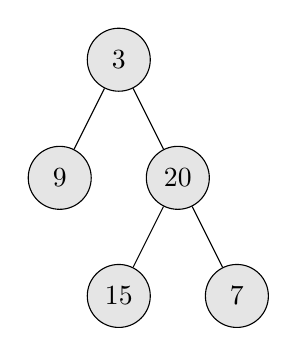
\begin{tikzpicture}
[every node/.style={draw, circle, fill=gray!20!, minimum size=8mm}]
\node{3}
child{node{9}}
child{node{20} child{node{15}} child{node{7}}};
\end{tikzpicture}
\end{figure}
\textbf{Output}: $[3, 14.5, 11]$

\textbf{Explanation}:

The average value of nodes on level 0 is 3,  on level 1 is 14.5, and on level 2 is 11. Hence return $[3, 14.5, 11]$.
\end{flushleft}

\paragraph{Note:}
\begin{itemize}
\item The range of node's value is in the range of 32-bit signed integer.
\end{itemize}

\subsection{BFS}
This is an easy question: just making use of breath first search with queue. 
% \section{638 --- Shopping Offers}
In LeetCode Store, there are some kinds of items to sell. Each item has a price.

However, there are some special offers, and a special offer consists of one or more different kinds of items with a sale price.

You are given the each item's price, $P$, a set of special offers, $S$, and the number we need to buy for each item, $N$. The job is to output the lowest price you have to pay for exactly certain items as given, where you could make optimal use of the special offers.

Each special offer is represented in the form of an array, the last number represents the price you need to pay for this special offer, other numbers represents how many specific items you could get if you buy this offer.

You could use any of special offers as many times as you want.

\paragraph{Example 1:}

\begin{flushleft}
\textbf{Input}: [2,5], [[3,0,5],[1,2,10]], [3,2]

\textbf{Output}: 14

\textbf{Explanation}:
 
There are two kinds of items, A and B. Their prices are \$2 and \$5 respectively. 

In special offer 1, you can pay \$5 for 3A and 0B

In special offer 2, you can pay \$10 for 1A and 2B. 

You need to buy 3A and 2B, so you may pay \$10 for 1A and 2B (special offer \#2), and \$4 for 2A.
\end{flushleft}

\paragraph{Example 2:}

\begin{flushleft}
\textbf{Input}: [2,3,4], [[1,1,0,4],[2,2,1,9]], [1,2,1]

\textbf{Output}: 11

\textbf{Explanation}: 

The price of A is \$2, and \$3 for B, \$4 for C. 

You may pay \$4 for 1A and 1B, and \$9 for 2A ,2B and 1C. 

You need to buy 1A ,2B and 1C, so you may pay \$4 for 1A and 1B (special offer \#1), and \$3 for 1B, \$4 for 1C. 

You cannot add more items, though only \$9 for 2A ,2B and 1C.
\end{flushleft}

\paragraph{Note:}

\begin{itemize}
\item There are at most 6 kinds of items, 100 special offers.
\item For each item, you need to buy at most 6 of them.
\item You are not allowed to buy more items than you want, even if that would lower the overall price.
\end{itemize}

\subsection{Backtracking}
From the question, 
\begin{itemize}
\item $N$ needs to be updated when applying any special offer.
\item One special offer can only be used only if the number items of each type is no larger than the ones available in the current $N$.
\item One special offer can be used more than once.
\end{itemize}

Therefore, in the recursion function to backtrack, 
\begin{enumerate}
\item We must test each special offer for current $N$. This means there will be a loop from given start index.
\item For each special offer that can be applied to current needs list $N$, updated $N$ and then recursively starting from this offer to test again. When the recursive calling is end, do backtrack, i.e., restore back $N$ to the ones before the recursive call.
\item After the loop ended, we may still have some items left to be purchased. Thus we add the remaining costs to the total cost and update the minimum one.
\end{enumerate}

% \section{639 --- Decode Ways II}
A message containing letters from A-Z is being encoded to numbers using the following mapping way:

\begin{table}[H]
\begin{tabular}{lc}
\hline
 A & 1 \\
B & 2\\
$\ldots$  & $\ldots$ \\
Z & 26 \\
\hline
\end{tabular}
\end{table}

Beyond that, now the encoded string can also contain the character $\ast$, which can be treated as one of the numbers from 1 to 9.

Given the encoded message containing digits and the character $\ast$, return the total number of ways to decode it.

Also, since the answer may be very large, you should return the output mod $10^9 + 7$.

\paragraph{Example 1:}

\begin{flushleft}
\textbf{Input}: $\ast$

\textbf{Output}: 9

Explanation: The encoded message can be decoded to the string: A, B, C, D, E, F, G, H, I.
\end{flushleft}

\paragraph{Example 2:}

\begin{flushleft}
Input: $1\ast$

Output: $9 + 9 = 18$

\end{flushleft}

\paragraph{Note:}

\begin{itemize}
\item The length of the input string will fit in range $[1, 10^5]$.
\item The input string will only contain the character $\ast$ and digits 0 to 9.
\end{itemize}


\subsection{Dynamic Programming}
Suppose $F[i]$ is the number of decode ways for string $S[0, i-1]$, then for $F[i+1]$, we can decode $S[i]$ with $S[i-1]$ and decode $S[i]$ only.

If we decode $S[i]$ with $S[i-1]$, there are three scenarios: 
\begin{enumerate}
\item If $S[i-1] = 1$, then $S[i-1]$ and $S[i]$ can be decoded together since $11$ to $19$ can represent valid letters. Thus, if $S[i]$ is in range $[0,9]$, $F[i]$ will add the result from $F[i-1]$. If $S[i]$ is $\ast$, then $F[i]$ will add $9\times F[i-1]$ since we can append 9 possible numbers from 1 to 9 to the decode results for $S[0,i-2]$.
\item If $S[i-1] = 2$, $S[i-1]$ and $S[i]$ can be decoded together only when $S[i]$ is in range $[0,6]$. Thus, if $S[i]$ is in range $[0,6]$, we add $F[i-1]$ to $F[i]$. If $S[i]$ is $\ast$, $F[i]$ will add $6 \times F[i-1]$ since we can append 6 possible numbers from 1 to 6 to the decode results for $S[0, i-2]$.
\item If $S[i-1]$ is $\ast$, then the choice of numbers to replace $\ast$ depends on $S[i]$.
\begin{itemize}
\item When $S[i]$ is in range $[0,6]$, we can choose 1 or 2 to replace $\ast$. Thus, we add $2\times F[i-1]$ to $F[i+1]$ for two possible numbers.
\item When $S[i]$ is in range $[7,9]$, we can only choose 1 to replace $\ast$. Then $F[i+1]$ is updated by adding $F[i-1]$.
\item When $S[i]$ is also $\ast$, we can choose between $[11,19]$ and $[21,26]$ to replace $S[i-1, i]$ because $\ast$ cannot be zero. Therefore, we have 15 possible numbers to append to the decode results for $S[0, i-2]$, which means $F[i+1]$ will be added by $15\times F[i-1]$.
\end{itemize}
\end{enumerate}

To decode $S[i]$ only, 

\begin{enumerate}
\item If $S[i]$ is between 1 and 9, just add $F[i]$ to $F[i+1]$ because each number represent only one letter.
\item If $S[i-1]$ is $\ast$, we will add $9\times F[i]$ to $F[i+1]$ since we have 9 possible numbers appending to the decode results for $S[0, i-1]$. 
\end{enumerate}

Lastly, for empty string, we set $F[0]=1$. From above description, we also see that $F[i+1]$ only depends on $F[i-1]$ and $F[i]$. Thus, we can use two variables to replace $F[i-1]$ and $F[i]$. 
% \section{640 --- Solve the Equation}
Solve a given equation and return the value of $x$ in the form of string $x=n$. The equation contains only plus, minus operation, the variable $x$ and its coefficient.

If there is no solution for the equation, return \textbf{No solution}.

If there are infinite solutions for the equation, return \textbf{Infinite solutions}.

If there is exactly one solution for the equation, we ensure that the value of $x$ is an integer.

\paragraph{Example 1:}

\begin{flushleft}
\textbf{Input}: $x+5-3+x=6+x-2$

\textbf{Output}: $x=2$

\end{flushleft}

\paragraph{Example 2:}

\begin{flushleft}
\textbf{Input}: $x=x$

\textbf{Output}: \textbf{Infinite solutions}

\end{flushleft}

\paragraph{Example 3:}

\begin{flushleft}
Input: $2x=x$

Output: $x=0$

\end{flushleft}

\paragraph{Example 4:}

\begin{flushleft}
\textbf{Input}: $2x+3x-6x=x+2$

\textbf{Output}: $x=-1$

\end{flushleft}

\paragraph{Example 5:}

\begin{flushleft}
\textbf{Input}: $x=x+2$

\textbf{Output}: \textbf{No solution}

\end{flushleft}

\subsection{Group Coefficients}
\begin{itemize}
\item Split the function per the equal sign.
\item Parse two expressions split by the equal sign.
\item Iterating the expression, whenever a plus or minus sign is met
\begin{enumerate}
\item Accumulate the coefficients of $x$ by checking if last letter is $x$.
\item If it is not, accumulate the values.
\end{enumerate}
\item To dealing with $0\times x$, we set the starting number as $-1$ to indicate whether a $x$ has a coefficient or not.
\end{itemize}
% \section{641 --- Design Circular Deque}
Design your implementation of the circular double-ended queue (deque).

Your implementation should support following operations:

\begin{itemize}
\item \lstinline[language=Java, basicstyle=\small\ttfamily, keywordstyle=\bfseries\color{green!40!black}]|MyCircularDeque(k)|: Constructor, set the size of the deque to be $k$.
\item \lstinline[language=Java, basicstyle=\small\ttfamily, keywordstyle=\bfseries\color{green!40!black}]|insertFront()|: Adds an item at the front of Deque. Return true if the operation is successful.
\item \lstinline[language=Java, basicstyle=\small\ttfamily, keywordstyle=\bfseries\color{green!40!black}]|insertLast()|: Adds an item at the rear of Deque. Return true if the operation is successful.
\item \lstinline[language=Java, basicstyle=\small\ttfamily, keywordstyle=\bfseries\color{green!40!black}]|deleteFront()|: Deletes an item from the front of Deque. Return true if the operation is successful.
\item \lstinline[language=Java, basicstyle=\small\ttfamily, keywordstyle=\bfseries\color{green!40!black}]|deleteLast()|: Deletes an item from the rear of Deque. Return true if the operation is successful.
\item \lstinline[language=Java, basicstyle=\small\ttfamily, keywordstyle=\bfseries\color{green!40!black}]|getFront()|: Gets the front item from the Deque. If the deque is empty, return $-1$.
\item \lstinline[language=Java, basicstyle=\small\ttfamily, keywordstyle=\bfseries\color{green!40!black}]|getRear()|: Gets the last item from Deque. If the deque is empty, return $-1$.
\item \lstinline[language=Java, basicstyle=\small\ttfamily, keywordstyle=\bfseries\color{green!40!black}]|isEmpty()|: Checks whether Deque is empty or not. 
\item \lstinline[language=Java, basicstyle=\small\ttfamily, keywordstyle=\bfseries\color{green!40!black}]|isFull()|: Checks whether Deque is full or not.
\end{itemize} 

\paragraph{Example:}

\begin{lstlisting}[style=customc]
MyCircularDeque circularDeque = new MycircularDeque( 3 ); // set the size to be 3
circularDeque.insertLast( 1 );			// return true
circularDeque.insertLast( 2 );			// return true
circularDeque.insertFront( 3 );			// return true
circularDeque.insertFront( 4 );			// return false, the queue is full
circularDeque.getRear();  			// return 2
circularDeque.isFull();				// return true
circularDeque.deleteLast();			// return true
circularDeque.insertFront( 4 );			// return true
circularDeque.getFront();			// return 4
\end{lstlisting}
 

\paragraph{Note:}

\begin{itemize}
\item All values will be in the range of [0, 1000].
\item The number of operations will be in the range of [1, 1000].
\item Please do not use the built-in Deque library.
\end{itemize}

\subsection{Two Pointers/Indexes}
\begin{itemize}
\item We make use of two pointers/ indexes: front and rear to track current begin and end of queue.
\item To simply the task, we also maintains a variable, say $z$, to track number of items in the queue.
\item At start, front is set to zero and rear to the last index ($k-1$) of the underlying array.
\item When insert into front, we set current slot of array at the index \texttt{front} to the given value, and then increments \texttt{front}. Also, we increment the number of items in the queue. 
\item Similarly, when insert into rear, set current lot at the index \texttt{rear} as the given value, and then decrements \texttt{rear}. We also increment the number of items in the queue.
\item For delete front and rear, the operation is reverse of insert. 
\item Since we maintain the number of items in the queue, it is easy to check if the queue is empty ($z=0$) or full ($z=k$).
\end{itemize}

% \section{642 --- Design Search Autocomplete System}
Design a search autocomplete system for a search engine. Users may input a sentence (at least one word and end with a special character \#). For \textbf{each character} they type \textbf{except} \#, you need to return the \textbf{top 3} historical hot sentences that have prefix the same as the part of sentence already typed. Here are the specific rules:

\begin{enumerate}
\item The hot degree for a sentence is defined as the number of times a user typed the exactly same sentence before.
\item The returned top 3 hot sentences should be sorted by hot degree (The first is the hottest one). If several sentences have the same degree of hot, you need to use ASCII-code order (smaller one appears first).
\item If less than 3 hot sentences exist, then just return as many as you can.
\item When the input is a special character, it means the sentence ends, and in this case, you need to return an empty list.
\end{enumerate}

Your job is to implement the following functions:

The constructor function:

\lstinline[language=Java, basicstyle=\small\ttfamily, keywordstyle=\bfseries\color{green!40!black}]|AutocompleteSystem(String[] sentences, int[] times)|: This is the constructor. The input is \textbf{historical data}. \texttt{Sentences} is a string array consists of previously typed sentences. \texttt{Times} is the corresponding times a sentence has been typed. Your system should record these historical data.

Now, the user wants to input a new sentence. The following function will provide the next character the user types:

\lstinline[language=Java, basicstyle=\small\ttfamily, keywordstyle=\bfseries\color{green!40!black}]|List<String> input(char c)|: The input \texttt{c} is the next character typed by the user. The character will only be lower-case letters (\texttt{a} to \texttt{z}), blank space or a special character (\#). Also, the previously typed sentence should be recorded in your system. The output will be the \textbf{top 3} historical hot sentences that have prefix the same as the part of sentence already typed.
 

\paragraph{Example:}

\begin{flushleft}

\textbf{Operation}:
 \lstinline[language=Java, basicstyle=\small\ttfamily, keywordstyle=\bfseries\color{green!40!black}]|AutocompleteSystem(["i love you", "island", "ironman", "i love leetcode"],[5, 3, 2, 2])|

The system have already tracked down the following sentences and their corresponding times:

\lstinline[language=Java, basicstyle=\small\ttfamily, keywordstyle=\bfseries\color{green!40!black}]|"i love you"| : 5 times

\lstinline[language=Java, basicstyle=\small\ttfamily, keywordstyle=\bfseries\color{green!40!black}]|"island"| : 3 times

\lstinline[language=Java, basicstyle=\small\ttfamily, keywordstyle=\bfseries\color{green!40!black}]|"ironman"| : 2 times

\lstinline[language=Java, basicstyle=\small\ttfamily, keywordstyle=\bfseries\color{green!40!black}]|"i love leetcode"| : 2 times

Now, the user begins another search:

\textbf{Operation}: \lstinline[language=Java, basicstyle=\small\ttfamily, keywordstyle=\bfseries\color{green!40!black}]|input('i')|

\textbf{Output}: \lstinline[language=Java, basicstyle=\small\ttfamily, keywordstyle=\bfseries\color{green!40!black}]|["i love you", "island", "i love leetcode"]|

\textbf{Explanation}:

There are four sentences that have prefix \texttt{i} . Among them, \lstinline[language=Java, basicstyle=\small\ttfamily, keywordstyle=\bfseries\color{green!40!black}]|"ironman"| and \lstinline[language=Java, basicstyle=\small\ttfamily, keywordstyle=\bfseries\color{green!40!black}]|"i love leetcode"| have same hot degree. Since letter \lstinline[language=Java, basicstyle=\small\ttfamily, keywordstyle=\bfseries\color{green!40!black}]|' '| has ASCII code 32 and \lstinline[language=Java, basicstyle=\small\ttfamily, keywordstyle=\bfseries\color{green!40!black}]|'r'| has ASCII code 114, \lstinline[language=Java, basicstyle=\small\ttfamily, keywordstyle=\bfseries\color{green!40!black}]|"i love leetcode"| should be in front of \lstinline[language=Java, basicstyle=\small\ttfamily, keywordstyle=\bfseries\color{green!40!black}]|"ironman"|. Also we only need to output top 3 hot sentences, so \lstinline[language=Java, basicstyle=\small\ttfamily, keywordstyle=\bfseries\color{green!40!black}]|"ironman"| will be ignored.

\textbf{Operation}: \lstinline[language=Java, basicstyle=\small\ttfamily, keywordstyle=\bfseries\color{green!40!black}]|input(' ')|

\textbf{Output}: \lstinline[language=Java, basicstyle=\small\ttfamily, keywordstyle=\bfseries\color{green!40!black}]|["i love you", "i love leetcode"]|

\textbf{Explanation}:

There are only two sentences that have prefix \lstinline[language=Java, basicstyle=\small\ttfamily, keywordstyle=\bfseries\color{green!40!black}]|"i "|

\textbf{Operation}: \lstinline[language=Java, basicstyle=\small\ttfamily, keywordstyle=\bfseries\color{green!40!black}]|input('a')|

\textbf{Output}: \lstinline[language=Java, basicstyle=\small\ttfamily, keywordstyle=\bfseries\color{green!40!black}]|[]|

\textbf{Explanation}:

There are no sentences that have prefix \lstinline[language=Java, basicstyle=\small\ttfamily, keywordstyle=\bfseries\color{green!40!black}]|"i a"|.

\textbf{Operation}: \lstinline[language=Java, basicstyle=\small\ttfamily, keywordstyle=\bfseries\color{green!40!black}]|input('#')|

\textbf{Output}: \lstinline[language=Java, basicstyle=\small\ttfamily, keywordstyle=\bfseries\color{green!40!black}]|[]|

\textbf{Explanation}:

The user finished the input, the sentence \lstinline[language=Java, basicstyle=\small\ttfamily, keywordstyle=\bfseries\color{green!40!black}]|"i a"| should be saved as a historical sentence in system. And the following input will be counted as a new search.
 

\end{flushleft}

\paragraph{Note:}

\begin{itemize}
\item The input sentence will always start with a letter and end with \#, and only one blank space will exist between two words.
\item The number of complete sentences that to be searched won't exceed 100. The length of each sentence including those in the historical data won't exceed 100.
\item Please use double-quote instead of single-quote when you write test cases even for a character input.
\end{itemize}

\subsection{Brute Force}
We make use of a hash map $M$ to store entries in the form $(S[i], T[i])$. Here, $T[i]$ is the number of times the sentence $S[i]$​ has been typed earlier.

\begin{itemize}
\item \lstinline[language=Java, basicstyle=\small\ttfamily, keywordstyle=\bfseries\color{green!40!black}]|AutocompleteSystem|: We pick up each sentence  and their corresponding times from the given inputs, and add to $M$.

\item \lstinline[language=Java, basicstyle=\small\ttfamily, keywordstyle=\bfseries\color{green!40!black}]|input(c)|: We make use of a variable, $x$ to store the sentence entered till now as the input. For current input character $c$, we append it to $x$ and then iterate over all the keys of $M$ to check if a key exists whose initial characters match with $x$ (In C++, we can use function \lstinline[language=Java, basicstyle=\small\ttfamily, keywordstyle=\bfseries\color{green!40!black}]|compare| to check if a key starts with $x$). We add all such keys to a list, $\ell$. Then, we sort $\ell$ as per our requirements, and obtain the first three values from it.
\end{itemize}

\subsection{Two Levels Hash Map}
Brute force is not an optimal one. To improve the efficiency, we instead make use of a two level hash map, i.e., an array, $A$, with each element as a hash map. The array's size is 26. For example, $A[0]$ is a hash map which stores the sentences starting with letter \texttt{a}.

The process remains the same as in the brute force approach, except the one level indexing of $A$ which needs to be done prior to accessing the required hash map.

\subsection{Trie}
Using Trie is very straight forward. We build a trie tree from the input sentences. We store the times and the string into the leaf node of the tree. 

Then for each input, we traverse the tree until a start node. Then from this node, we collect all reachable leaf nodes, put the times and string into a tree map to automatically sort by the times. The value of each node in the tree map is a tree set so that we can sort the strings with same times automatically. 
% \section{643 --- Maximum Average Subarray I}
Given an array consisting of $n$ integers, $A$, find the contiguous subarray of given length $k$ that has the maximum average value. And you need to output the maximum average value.

\paragraph{Example 1:}

\begin{flushleft}
\textbf{Input}: $[1,12,-5,-6,50,3]$, $k = 4$

\textbf{Output}: 12.75

\textbf{Explanation}: Maximum average is $(12-5-6+50)/4 = 51/4 = 12.75$

\end{flushleft}
 

\paragraph{Note:}

\begin{itemize}
\item $1 \leq k \leq n \leq 30,000$.
\item Elements of the given array will be in the range $[-10,000, 10,000]$.
\end{itemize}

\subsection{Sliding Window}
Assume that we already know the sum of elements from index $i$ to index $i+k$, say it is $x$.

Now, to determine the sum of elements from the index $i+1$ to the index $i+k+1$, all we need to do is to subtract the element $A[i]$ from $x$ and to add the element $A[i+k+1]$ to $x$. We can carry out our process based on this idea and determine the maximum possible average.
% \section{644 --- Maximum Average Subarray II}
Given an array consisting of $n$ integers, $A$, find the contiguous subarray whose length is greater than or equal to $k$ that has the maximum average value. And you need to output the maximum average value.

\paragraph{Example 1:}

\begin{flushleft}
\textbf{Input}: $[1,12,-5,-6,50,3]$, $k = 4$

\textbf{Output}: 12.75

\textbf{Explanation}:

when length is 5, maximum average value is 10.8,

when length is 6, maximum average value is 9.16667.

Thus return 12.75.
\end{flushleft}

\paragraph{Note:}

\begin{itemize}
\item $1 \leq k \leq n \leq 10,000$.
\item Elements of the given array will be in range $[-10,000, 10,000]$.
\item The answer with the calculation error less than $10^{-5}$ will be accepted.
\end{itemize}

\subsection{Binary Search}
\begin{enumerate}
\item Notice that the value of the average could lie between a range $[\min(A),\max(A)]$. Here, $x$ and $y$ refer to the minimum and the maximum values out of the given array $A$. \item To find the maximum average of a subarray with at least $k$ elements, we can try to guess and test if a value close to the real maximum average. This will fits a Binary Search approach since we know the range of the real maximum average.
\item During the search, suppose $z$ is the middle value in current range $[x,y]$, i.e., $z=(x+y)/2$, then the task is to find if a subarray with length greater than or equal to $k$ is possible with an average greater than $z$.
\begin{itemize}
\item Now assume there is a subarray $A[i, i+m-1]$ (length is $m\geq k$) such that its average is greater than $z$, i.e, 

$$(A[i] + A[i+1] + \ldots +A[i+m-1])/ m \geq z$$

By transforming this inequality equation, we have 
\begin{align*}
A[i] + A[i+1] + \ldots +A[i+m-1] & \geq m\times z \\
(A[i] - z) + (A[i+1]-z) + \ldots + (A[i+m-1]-z) &\geq 0
\end{align*} 

Thus, for any subarray with length no less than $k$, if subtracting $z$ from each element inside and the summation after is still no less than zero, this means the average value of this subarray is greater than the middle value $z$. Hence, we need to search in the upper half of current range. Otherwise, we will find in the lower hal.
\end{itemize}

\end{enumerate}

In order to determine if such a subarray exists in a linear manner, we maintain a variable, say $\alpha$, to store the summation of $A[i]-z$ until the $i$-th element while traversing over $A$. 

If $(A[0]-z) +\ldots +(A[k-1]-z)\geq 0$, we know the average can be increased over $z$, thus we can directly search in upper half range. Otherwise, we continue from  $A[k]$ until last element, by making use of the following idea.

\begin{itemize}
\item If we know the summation of $A[i]-z$ and $A[j]-z$, say $\alpha_i$ and $\alpha_j$, then we have $(A[i+1]-z) + (A[i+2]-z)+\ldots+(A[j]-z) = \alpha_j - \alpha_i$. Thus we need to find if $\alpha_j - \alpha_i\geq 0 $ for $j-i \geq k$.
\item Instead of checking all possible values of $\alpha$ for each index, we just consider the minimum $\alpha$ until the index $j-k$. 
\item So, we maintain a variable $\beta$ to store the cumulative summation of $A[i-k]-z$ for each index $i$, and we also record the minimum of $\beta$.
\end{itemize}

There is one more thing to note: in this binary search, we are comparing \lstinline[language=Java, basicstyle=\small\ttfamily, keywordstyle=\bfseries\color{green!40!black}]|double| type. Thus, we need to compare the difference with some predefined precision. The problem requires less than $10^{-5}$, so the process will stop when we get error below than $0.00001$.

% \section{645 --- Set Mismatch}
The set $S$ originally contains numbers from 1 to $n$. But unfortunately, due to the data error, one of the numbers in the set got duplicated to another number in the set, which results in repetition of one number and loss of another number.

Given an array $A$ representing the data status of this set after the error. Your task is to firstly find the number occurs twice and then find the number that is missing. Return them in the form of an array.

\paragraph{Example 1:}

\begin{flushleft}
\textbf{Input}: $A = [1,2,2,4]$

\textbf{Output}: $[2,3]$
\end{flushleft}

\paragraph{Note:}

\begin{itemize}
\item The given array size will in the range [2, 10000].
\item The given array's numbers won't have any order.
\end{itemize}

\subsection{Index By Itself}
This approach has been appeared in previous problems. 

\begin{itemize}
\item Traverse the array, for each element $A[i]$, we multiply $A[A[i]-1]$ by $-1$. If $A[A[i]-1]$ is already a negative number, then the duplicate number is $A[i]-1$.
\item Traverse the array again, if an element, say $A[k]$ is larger than zero, $k+1$ is the missing number.
\end{itemize}

\subsection{XOR}
Consider an array $D$ with $n−1$ elements containing numbers from $1$ to $n$ with one number missing out of them. To find the missing one, we can take the XOR of all the elements of $D$ with all the numbers from $1$ to $n$. By doing so, we get the required missing number. This works because XOR of two same numbers are zero. Thus, only the number which is missing can't get canceled by XOR.

Now, By taking the XOR of all the elements of the given array $A$ with all the numbers from 1 to $n$, we will get a result, $z$, as \lstinline[language=Java, basicstyle=\small\ttfamily, keywordstyle=\bfseries\color{green!40!black}]|x ^ y|. Here, $x$ and $y$ refer to the repeated and the missing term in $A$.

Now, we'll get a 1 in the binary representation of $z$ only at those bit positions which have a 1 in either $x$ or $y$, and a 0 at the same bit position in the other one. For this problem, we consider the rightmost bit position, $b$, which is 1 in $z$, although any bit would work.

If we divide the elements of $A$ into two parts such that the first set contains the elements which have a 1 at bit position $b$ and the second set contains the elements having a 0 at the same position, we'll get $x$ from one set and $y$ from another. Thus, we test $1$ to $n$ and all elements in $A$ by checking their bit position $b$.

\begin{itemize}
\item XOR all the numbers with value 1 in the bit position $b$ to get a result $\alpha$.
\item XOR all the numbers with value 0 in the bit position $b$ to get a result $\beta$.
\end{itemize}

But, we don't know which one is missing and which one is duplicate. We have to iterate over $A$ again to check if $\alpha$ or $\beta$ appear in the array.

% \section{646 --- Maximum Length of Pair Chain}
You are given $n$ pairs of numbers. In every pair, the first number is always smaller than the second number.

Now, we define a pair $(c, d)$ can follow another pair $(a, b)$ if and only if $b < c$. Chain of pairs can be formed in this fashion.

Given a set of pairs, find the length longest chain which can be formed. You needn't use up all the given pairs. You can select pairs in any order.

\paragraph{Example 1:}

\begin{flushleft}
\textbf{Input}: [[1,2], [2,3], [3,4]]

\textbf{Output}: 2

\textbf{Explanation}: The longest chain is [1,2] $\longrightarrow$ [3,4]

\end{flushleft}

\paragraph{Note:}

\begin{itemize}
\item The number of given pairs will be in the range [1, 1000].
\end{itemize}

\subsection{Dynamic Programming}
If a chain of length $k$ ends at some \lstinline[language=C++, basicstyle=\small\ttfamily, keywordstyle=\bfseries\color{green!40!black}]|pairs[i]|, and \lstinline[language=C++, basicstyle=\small\ttfamily, keywordstyle=\bfseries\color{green!40!black}]|pairs[i][1] < pairs[j][0]|, we can extend this chain to a chain of length $k+1$. This is same approach as finding longest increasing subsequence. Note that we needs to sort the input pairs first.

\subsection{Greedy}
If we view these pairs as ranges with start and end time, this problem will be same as find maximum non-overlap ranges. In this approach, we sort the input pairs array per the end time (second element). Maintain a variable to record current range's end. If a range has a start time larger than current end time, we know we find a new  non-overlapped range, so increments the result.




% \section{647 --- Palindromic Substrings}

Given a string, $S$, your task is to count how many palindromic substrings in this string.

The substrings with different start indexes or end indexes are counted as different substrings even they consist of same characters.

\paragraph{Example 1:}
\begin{flushleft}
\textbf{Input}: \lstinline[language=C++, basicstyle=\small\ttfamily, keywordstyle=\bfseries\color{green!40!black}]|"abc"|

\textbf{Output}: 3

\textbf{Explanation}: Three palindromic strings: \lstinline[language=C++, basicstyle=\small\ttfamily, keywordstyle=\bfseries\color{green!40!black}]|"a", "b", "c"|.
\end{flushleft}
 

\section{Example 2:}
\begin{flushleft}
\textbf{Input}: \lstinline[language=C++, basicstyle=\small\ttfamily, keywordstyle=\bfseries\color{green!40!black}]|"aaa"|

\textbf{Output}: 6

\textbf{Explanation}: Six palindromic strings: \lstinline[language=C++, basicstyle=\small\ttfamily, keywordstyle=\bfseries\color{green!40!black}]|"a", "a", "a", "aa", "aa", "aaa"|.
\end{flushleft}
 

\paragraph{Note:}
\begin{itemize}
    \item The input string length won't exceed 1000.
\end{itemize}

\subsection{Dynamic Programming}
We can make use of 2-d dynamic programming with an 2-d array $F[i][j]$ to indicate if sub-string $s[i,j]$ is a palindrome or not. If it is, we increments the results.

\subsection{Expand Around Center}
We can also use $O(1)$ memory space. In this approach, Let $\ell$ be the length of the string. The middle of the palindrome could be in one of $2\ell - 1$ positions: \begin{itemize}
\item either at each letter: we have $\ell$ letters as centers for odd length palindromes.
\item or between two letters: we have $\ell$-1 positions between two consecutive letters for even length palindromes.
\end{itemize}

Count all the palindromes around each center. Notice that if $s[i, j]$ is a palindromic sub-string, then $s[i+1, j-1]$ is a palindrome too.



% \section{648 --- Replace Words}
In English, we have a concept called \textbf{root}, which can be followed by some other words to form another longer word - let's call this word \textbf{successor}. For example, the root \textbf{an}, followed by \textbf{other}, which can form another word \textbf{another}.

Now, given a dictionary consisting of many roots and a sentence. You need to replace all the successor in the sentence with the root forming it. If a successor has many roots can form it, replace it with the root with the shortest length.

You need to output the sentence after the replacement.

\paragraph{Example 1:}

\begin{flushleft}
\textbf{Input}: 

\lstinline[language=Java, basicstyle=\small\ttfamily, keywordstyle=\bfseries\color{green!40!black}]|dict = ["cat", "bat", "rat"]|

\lstinline[language=Java, basicstyle=\small\ttfamily, keywordstyle=\bfseries\color{green!40!black}]|sentence = "the cattle was rattled by the battery"|

\textbf{Output}: \lstinline[language=Java, basicstyle=\small\ttfamily, keywordstyle=\bfseries\color{green!40!black}]|"the cat was rat by the bat"|

\end{flushleft}
 

\paragraph{Note:}

\begin{itemize}
\item The input will only have lower-case letters.
\item $1 \leq W \leq 1000$, where $W$ is the number of dict words.
\item $1 \leq S \leq 1000$, where $S$ is the number of sentence words.
\item $1 \leq R \leq 100$, where $R$ is the length of root.
\item $1 \leq L \leq 1000$, where $L$ is the length of each sentence word.
\end{itemize}

\subsection{Trie}
This coding question is a typical application of trie tree.
% \section{649 --- Dota2 Senate}
In the world of \textbf{Dota2}, there are two parties: the \textbf{Radiant} and the \textbf{Dire}.

The \textbf{Dota2} senate consists of senators coming from two parties. Now the senate wants to make a decision about a change in the \textbf{Dota2} game. The voting for this change is a round-based procedure. In each round, each senator can exercise one of the two rights:
\begin{enumerate}
\item \textit{Ban one senator's right}: A senator can make another senator lose \textbf{all his rights} in this and all the following rounds.
\item \textit{Announce the victory}: If this senator found the senators who still have rights to vote are all from \textbf{the same party}, he can announce the victory and make the decision about the change in the game.
\end{enumerate}

Given a string $S$ representing each senator's party belonging. The character \lstinline[language=Java, basicstyle=\small\ttfamily, keywordstyle=\bfseries\color{green!40!black}]|'R'| and \lstinline[language=Java, basicstyle=\small\ttfamily, keywordstyle=\bfseries\color{green!40!black}]|'D'| represent the \textbf{Radiant} party and the \textbf{Dire} party respectively. Then if there are $n$ senators, the size of the given string will be $n$.

The round-based procedure starts from the first senator to the last senator in the given order. This procedure will last until the end of voting. All the senators who have lost their rights will be skipped during the procedure.

Suppose every senator is smart enough and will play the best strategy for his own party, you need to predict which party will finally announce the victory and make the change in the Dota2 game. The output should be \textbf{Radiant} or \textbf{Dire}.

\paragraph{Example 1:}

\begin{flushleft}
\textbf{Input}: \lstinline[language=Java, basicstyle=\small\ttfamily, keywordstyle=\bfseries\color{green!40!black}]|"RD"|

\textbf{Output}: \lstinline[language=Java, basicstyle=\small\ttfamily, keywordstyle=\bfseries\color{green!40!black}]|"Radiant"|

\textbf{Explanation}: 

The first senator comes from Radiant and he can just ban the next senator's right in the round 1. 

And the second senator can't exercise any rights any more since his right has been banned. 

And in the round 2, the first senator can just announce the victory since he is the only guy in the senate who can vote.
\end{flushleft}


\paragraph{Example 2:}

\begin{flushleft}
\textbf{Input}: \lstinline[language=Java, basicstyle=\small\ttfamily, keywordstyle=\bfseries\color{green!40!black}]|"RDD"|

\textbf{Output}: \lstinline[language=Java, basicstyle=\small\ttfamily, keywordstyle=\bfseries\color{green!40!black}]|"Dire"|

\textbf{Explanation}: 

The first senator comes from Radiant and he can just ban the next senator's right in the round 1. 

And the second senator can't exercise any rights anymore since his right has been banned. 

And the third senator comes from Dire and he can ban the first senator's right in the round 1. 

And in the round 2, the third senator can just announce the victory since he is the only guy in the senate who can vote.
\end{flushleft}

\paragraph{Note:}

\begin{itemize}
\item     The length of the given string will in the range [1, 10,000].
\end{itemize}

\subsection{Simulation}
A senator performing a ban doesn't need to use it on another senator immediately. We can wait to see when another team's senator will vote, then use that ban retroactively.

We make use of a queue. At start, put all the senators into the queue. Then, process the queue, if there is a floating ban for that senator, exercise it and continue. Otherwise, add a floating ban against the other team, and enqueue this senator again.


% \section{650 --- 2 Keys Keyboard}
Initially on a notepad only one character \lstinline[language=Java, basicstyle=\small\ttfamily, keywordstyle=\bfseries\color{green!40!black}]|'A'| is present. You can perform two operations on this notepad for each step:

\begin{enumerate}
\item \textbf{Copy All}: You can copy all the characters present on the notepad (partial copy is not allowed).
\item \textbf{Paste}: You can paste the characters which are copied \textbf{last time}.

\end{enumerate}
 
Given a number $n$. You have to get exactly $n$ \lstinline[language=Java, basicstyle=\small\ttfamily, keywordstyle=\bfseries\color{green!40!black}]|'A'| on the notepad by performing the minimum number of steps permitted. Output the minimum number of steps to get $n$ \lstinline[language=Java, basicstyle=\small\ttfamily, keywordstyle=\bfseries\color{green!40!black}]|'A'|.

\paragraph{Example 1:}

\begin{flushleft}
\textbf{Input}: 3

\textbf{Output}: 3

\textbf{Explanation}:

Initially, we have one character \lstinline[language=Java, basicstyle=\small\ttfamily, keywordstyle=\bfseries\color{green!40!black}]|'A'|.

In step 1, we use Copy All operation.

In step 2, we use Paste operation to get \lstinline[language=Java, basicstyle=\small\ttfamily, keywordstyle=\bfseries\color{green!40!black}]|'AA'|.

In step 3, we use Paste operation to get \lstinline[language=Java, basicstyle=\small\ttfamily, keywordstyle=\bfseries\color{green!40!black}]|'AAA'|.

\end{flushleft}

\subsection{Prime Factorization}
We can break the moves into groups of (copy, paste, \textellipsis, paste). Let $C$ denote copying and $P$ denote pasting. For example, in the sequence of moves $CPPCPPPPCP$, the groups would be $[CPP]$, $[CPPPP]$, and $[CP]$.

Suppose we have $n$ such groups with lengths $g_1$, $g_2$, $\ldots$, $g_n$ respectively. After parsing the first group, there are $g_1$ \lstinline[language=Java, basicstyle=\small\ttfamily, keywordstyle=\bfseries\color{green!40!black}]|'A'|. After parsing the second group, there are $g_1 \times g_2$ \lstinline[language=Java, basicstyle=\small\ttfamily, keywordstyle=\bfseries\color{green!40!black}]|'A'|s, and so on. At the end, there are $g_1 \times g_2 \times g_n$ \lstinline[language=Java, basicstyle=\small\ttfamily, keywordstyle=\bfseries\color{green!40!black}]|'A'|.

Suppose the given $N = g_1 \times g_2\times \ldots g_k$. If any of the $g_i$ are composite, i.e., $g_i = p \times q$, we can split this group with length $g_i$ into two groups (the first of which has one \textbf{copy} followed by $p-1$ \textbf{pastes}, while the second group having one \textbf{copy} and $q-1$ \textbf{pastes}).

Such a split is the minimum moves we can get for getting $g_i$ \lstinline[language=Java, basicstyle=\small\ttfamily, keywordstyle=\bfseries\color{green!40!black}]|'A'|, because there are  $p+q$ compared with $p\times q$ operations. Based on inequality formula, $p+q \leq p\times q$ when $p\geq 2$ and $q\geq 2$..

Thus, the minimum operations for getting $N$ \lstinline[language=Java, basicstyle=\small\ttfamily, keywordstyle=\bfseries\color{green!40!black}]|'A'|, we just do the prime factorization of $N$, and the summation of these factors are the answer.

To find the prime factorization, we don't need to test each prime number.  We can 
\begin{enumerate}
\item start by testing the factor $x=2$, 
\item keep dividing $N$ by current factor $x$ until $N$ cannot be divided by $x$. 
\item Increments $x$
\item Go to step 2
\item If $N$ is 1, stop the process
\end{enumerate}
% \section{651 --- 4 Keys Keyboard}
Imagine you have a special keyboard with the following keys:

\begin{itemize}
\item Key 1: \lstinline[language=Java, basicstyle=\small\ttfamily, keywordstyle=\bfseries\color{green!40!black}]|(A)|: Print one \lstinline[language=Java, basicstyle=\small\ttfamily, keywordstyle=\bfseries\color{green!40!black}]|'A'| on screen.

\item Key 2: \lstinline[language=Java, basicstyle=\small\ttfamily, keywordstyle=\bfseries\color{green!40!black}]|(Ctrl-A)|: Select the whole screen.

\item Key 3: \lstinline[language=Java, basicstyle=\small\ttfamily, keywordstyle=\bfseries\color{green!40!black}]|(Ctrl-C)|: Copy selection to buffer.

\item Key 4: \lstinline[language=Java, basicstyle=\small\ttfamily, keywordstyle=\bfseries\color{green!40!black}]|(Ctrl-V)|: Print buffer on screen appending it after what has already been printed.
\end{itemize}

Now, you can only press the keyboard for $N$ times (with the above four keys), find out the maximum numbers of \lstinline[language=Java, basicstyle=\small\ttfamily, keywordstyle=\bfseries\color{green!40!black}]|'A'| you can print on screen.

\paragraph{Example 1:}

\begin{flushleft}
\textbf{Input}: $N = 3$

\textbf{Output}: 3

\textbf{Explanation}: 

We can at most get 3 \lstinline[language=Java, basicstyle=\small\ttfamily, keywordstyle=\bfseries\color{green!40!black}]|A| on screen by pressing following key sequence: \lstinline[language=Java, basicstyle=\small\ttfamily, keywordstyle=\bfseries\color{green!40!black}]|A, A, A|
\end{flushleft}

\paragraph{Example 2:}

\begin{flushleft}
\textbf{Input}: $N = 7$

\textbf{Output}: 9

\textbf{Explanation}: 

We can at most get 9 \lstinline[language=Java, basicstyle=\small\ttfamily, keywordstyle=\bfseries\color{green!40!black}]|A| on screen by pressing following key sequence:

\lstinline[language=Java, basicstyle=\small\ttfamily, keywordstyle=\bfseries\color{green!40!black}]|A, A, A, Ctrl A, Ctrl C, Ctrl V, Ctrl V|
\end{flushleft}

\paragraph{Note:}

\begin{itemize}
\item $1 \leq N \leq 50$
\item Answers will be in the range of 32-bit signed integer.
\end{itemize}

\subsection{Dynamic Programming}
Suppose $F[k]$ is the largest number of \lstinline[language=Java, basicstyle=\small\ttfamily, keywordstyle=\bfseries\color{green!40!black}]|'A'| after $k$ key presses.

If the last pressed key is 1, then $F[k] = F[k-1]+1$.

Otherwise, if the last pressed key was 4, i.e. paste operation, we will have $F[k-(x+1)] = F[k-(x+1)] \times x$ for some $x < k-1$, where $x$ is the number of \lstinline[language=Java, basicstyle=\small\ttfamily, keywordstyle=\bfseries\color{green!40!black}]|'A'| copied into the memory. Since press key 4 requires one key press, $x$ is acquired before $(k-1)$th key press. We need a loop to find $F[k]$ for index $j$ such that $1\leq j < k-1$.

\subsection{Optimized Dynamic Programming}
If we multiply by $2\times N$, paying a cost of $2\times N+1$, we could instead multiply by $N$ then 2, paying $N+4$. When $N \geq 3$, we don't pay more by doing it the second way.

Similarly, if we are to multiply by $2\times N+1$ paying $2\times N+2$, we could instead multiply by $N+1$ then 2, paying $N+5$. Again, when $N \geq 3$, we don't pay more doing it the second way.

Thus, we never multiply by more than 5, and then the recursive function $F[k] = \max(F[i-4]\times 3, F[i-5]\times 4)$. We can manually find $F[1]$ to $F[6]$, and use these as the start for $k\geq 7$.

\subsection{Mathematical Way}

When N is arbitrarily large, the long run behavior of multiplying by $k$ repeatedly is to get to the value
$k^{\dfrac{N}{k+1}}$​. Analyzing the function $k^{\dfrac{1}{k+1}}$ at values $k=2,3,4,5$, it attains a peak at $k=4$. Thus, we should expect that eventually, $F[K] = F[K-5] \times 4$.

A few more deductions can be made

\begin{itemize}
\item We never add after multiplying: if we add $c$ after multiplying by $k$, we should instead multiply by $k+c$.

\item We never add after 5: If we add 1 then multiply by $k$ to get to $(x+1) \times k = xk + k$, we could instead multiply by $k+1$ to get to $xk + x$. Since $k \leq 5$, we must have $x \leq 5$ for our additions to not be dominated.

\item The number of multiplications by 2, 3, or 5 is bounded.

\item Every time we've multiplied by 2 two times, we prefer to multiply by 4 once for less cost. ($4^1$ for a cost of 5, vs $2^2$ for a cost of 6.)
\item Every time we've multiplied by 3 five times, we prefer to multiply by 4 four times for the same cost but a larger result. ($4^4 > 3^5$, and cost is 20.)

\item Every time we've multiplied by 5 five times, we prefer to multiply by 4 six times for the same cost but a larger result. ($4^6 > 5^5$, and cost is 30.)
\end{itemize}

Together, this shows there are at most 5 additions and 9 multiplications by a number that isn't 4.

We can find the first 14 operations on 1 by hand: 1, 2, 3, 4, 5, 6, 9, 12, 16, 20, 27, 36, 48, 64, 81. After that, every subsequent number is achieved by multiplying by 4: i.e., $F[K] = F[K-5] \times 4$.

% \section{652 --- Find Duplicate Subtrees}
Given a binary tree, return all duplicate subtrees. For each kind of duplicate subtrees, you only need to return the root node of any one of them.

Two trees are duplicate if they have the same structure with same node values.

\paragraph{Example 1:}

\begin{flushleft}
\begin{figure}[H]
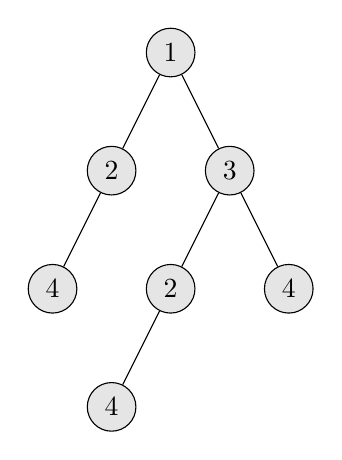
\begin{tikzpicture}
[every node/.style={draw, circle, fill=gray!20!, minimum size=5mm}]
\node{1}
child{node{2} child{node{4}} child[missing]}
child{node{3} child{node{2} child{node{4}} child[missing]} child{node{4}}};
\end{tikzpicture}
\end{figure}

The following are two duplicate subtrees:

\begin{figure}[H]
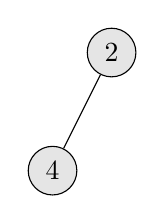
\begin{tikzpicture}
[every node/.style={draw, circle, fill=gray!20!, minimum size=5mm}]
\node{2}
child{node{4}}
child[missing];
\end{tikzpicture}
\end{figure}

\begin{figure}[H]
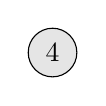
\begin{tikzpicture}
[my/.style={draw, circle, fill=gray!20!, minimum size=5mm}]
\node[my]{4};
\end{tikzpicture}
\end{figure}

Therefore, you need to return above trees' root in the form of a list.
\end{flushleft}

\subsection{Depth First Search}
This approach makes use of DFS to serialize a tree. The result string will be the unique string for this tree. For example, we can serialize the following tree 

\begin{figure}[H]
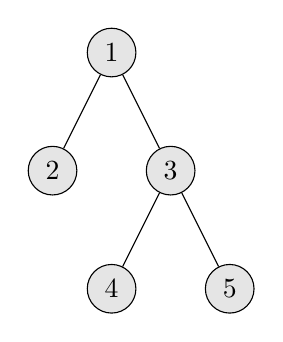
\begin{tikzpicture}
[every node/.style={draw, circle, fill=gray!20!, minimum size=5mm}]
\node{1}
child{node{2}}
child{node{3} child{node{4}} child{node{5}}};
\end{tikzpicture}
\end{figure}

as \lstinline[language=Java, basicstyle=\small\ttfamily, keywordstyle=\bfseries\color{green!40!black}]|1,2,#,#,3,4,#,#,5,#,#|

Thus, we can make use of a hash map to record the count of the same unique strings. When that count is larger than 1, we know we find a duplicate tree. Since we only output one of the root in these trees, we add the node into the output list only when the count is equal to 2.

\subsection{Optimized UUID}
Suppose we have a unique identifier for subtrees: two subtrees are the same if and only if they have the same id.

Then, for a node with left child id of $x$ and right child id of $y$, \lstinline[language=Java, basicstyle=\small\ttfamily, keywordstyle=\bfseries\color{green!40!black}]|(node.val, x, y)| uniquely determines the tree.

In this approach, we make use of two hash maps, say $m_1$ and $m_2$. 
\begin{itemize}
\item $m_1$ record the serialized string of a tree and its related uuid
\item $m_2$ map a tree's uuid to its count.
\end{itemize}

After getting the serialize result of a tree, search its uuid in $m_1$. If this is a new tree, create a new one. Then, we search the uuid in $m_2$. Similar to dfs approach, when this count reaches 2, we add current node into the output list.

% \section{653 --- Two Sum IV - Input is a BST}
Given a Binary Search Tree and a target number, return \lstinline[language=C++, basicstyle=\small\ttfamily, keywordstyle=\bfseries\color{green!40!black}]|true| if there exist two elements in the BST such that their sum is equal to the given target.

\paragraph{Example 1:}

\begin{flushleft}
\textbf{Input}: 
\begin{figure}[H]
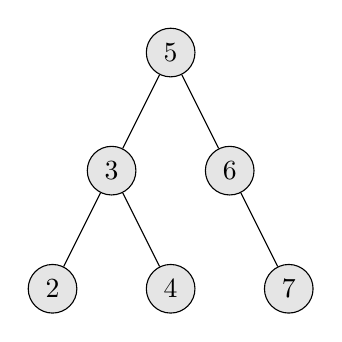
\begin{tikzpicture}
[every node/.style={draw, circle, fill=gray!20!, minimum size=5mm}]
\node{5}
child{node{3} child{node{2}} child{node{4}}}
child{node{6} child[missing] child{node{7}}};
\end{tikzpicture}
\end{figure}

\lstinline[language=C++, basicstyle=\small\ttfamily, keywordstyle=\bfseries\color{green!40!black}]|Target = 9|

\textbf{Output}: \lstinline[language=C++, basicstyle=\small\ttfamily, keywordstyle=\bfseries\color{green!40!black}]|true|
\end{flushleft}

 

\paragraph{Example 2:}

\textbf{Input}: 
\begin{figure}[H]
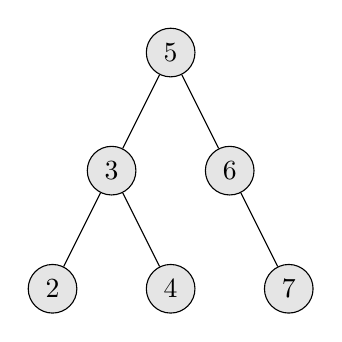
\begin{tikzpicture}
[every node/.style={draw, circle, fill=gray!20!, minimum size=5mm}]
\node{5}
child{node{3} child{node{2}} child{node{4}}}
child{node{6} child[missing] child{node{7}}};
\end{tikzpicture}
\end{figure}

\lstinline[language=C++, basicstyle=\small\ttfamily, keywordstyle=\bfseries\color{green!40!black}]|Target = 28|

\textbf{Output}: \lstinline[language=C++, basicstyle=\small\ttfamily, keywordstyle=\bfseries\color{green!40!black}]|false|

\subsection{Hash Set and Inorder Traverse}
We can traverse the tree by inorder approach, and make use of a hash set to store each node's value. When traversing, if the result of $k$ minus current node's value can be found in the hash set, it means there exists two numbers such that the sum of them is $k$.

\subsection{Convert To Sorted Array}
Since the given tree is a BST, the inorder traverse will give a sorted list (array). We can then use two pointers (indices) from both ends to check if there are two numbers whose sum is $k$.

% \section{654 --- Maximum Binary Tree}
Given an integer array with no duplicates. A maximum tree building on this array is defined as follow:

\begin{itemize}
\item The root is the maximum number in the array.
\item The left subtree is the maximum tree constructed from left part subarray divided by the maximum number.
\item The right subtree is the maximum tree constructed from right part subarray divided by the maximum number.

\end{itemize}
Construct the maximum tree by the given array and output the root node of this tree.

\paragraph{Example 1:}

\begin{flushleft}
\textbf{Input}: \lstinline[language=C++, basicstyle=\small\ttfamily, keywordstyle=\bfseries\color{green!40!black}]|[3,2,1,6,0,5]|

\textbf{Output}: return the tree root node representing the following tree:

\begin{figure}[H]
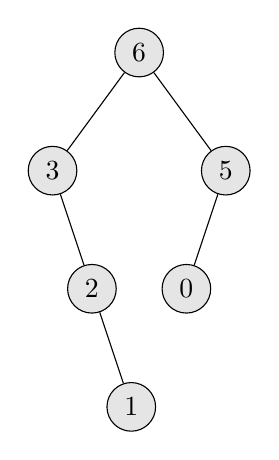
\begin{tikzpicture}
[every node/.style={draw, circle, fill=gray!20!, minimum size=5mm},
level 1/.style={sibling distance=22mm},
level 2/.style={sibling distance=10mm}]
\node{6}
child{node{3} child[missing] child{node{2} child[missing] child{node{1}}}}
child{node{5} child{node{0}} child[missing]};
\end{tikzpicture}
\end{figure}
\end{flushleft}

\paragraph{Note:}

\begin{itemize}
\item The size of the given array will be in the range \lstinline[language=Java, basicstyle=\small\ttfamily, keywordstyle=\bfseries\color{green!40!black}]|[1,1000]|.
\end{itemize}

\subsection{Divide And Conquer}
Divide the array into two halves per the maximum element. Recursively calling build function to create the maximum tree for each half.

\subsection{Using Stack}
In this approach, we make use of a stack to track local maximum during traversing the array
\begin{enumerate}
\item Create a new node for current element
\item Keep pop the top node from the stack as long as the it's value is less than current element. Also, set this top node as current node's left child.
\item After step 2 is completed, set current node as the right child of current top node of the stack. The top node of the stack is the local maximum.
\item Push current node into the stack.
\item After traversing is done, return the bottom of the stack as the root node.
\end{enumerate}

% \section{655 --- Print Binary Tree}
Print a binary tree in an $m\times n$ 2D string array following these rules:

\begin{enumerate}
\item The row number $m$ should be equal to the height of the given binary tree.
\item The column number $n$ should always be an odd number.
\item The root node's value (in string format) should be put in the exactly middle of the first row it can be put. The column and the row where the root node belongs will separate the rest space into two parts (\textbf{left-bottom part and right-bottom part}). You should print the left subtree in the left--bottom part and print the right subtree in the right--bottom part. The left-bottom part and the right-bottom part should have the same size. Even if one subtree is none while the other is not, you don't need to print anything for the none subtree but still need to leave the space as large as that for the other subtree. However, if two subtrees are none, then you don't need to leave space for both of them.
\item Each unused space should contain an empty string \lstinline[language=C++, basicstyle=\small\ttfamily, keywordstyle=\bfseries\color{green!40!black}]|""|.
\item Print the subtrees following the same rules.
\end{enumerate}

\paragraph{Example 1:}

\begin{flushleft}
\textbf{Input}:
\begin{figure}[H]
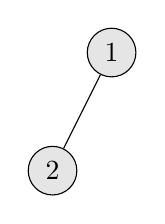
\begin{tikzpicture}
[every node/.style={draw, circle, fill=gray!20!, minimum size=5mm}]
\node{1}
child{node{2}}
child[missing];
\end{tikzpicture}
\end{figure}

\textbf{Output}:
\begin{lstlisting}[style=customc, caption={}]
{
["", "1", ""],
["2", "", ""]
}
\end{lstlisting}
\end{flushleft}

\paragraph{Example 2:}

\begin{flushleft}
\textbf{Input}:
\begin{figure}[H]
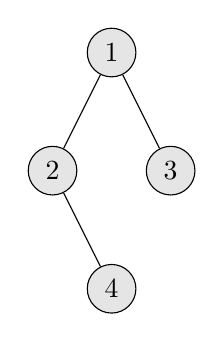
\begin{tikzpicture}
[every node/.style={draw, circle, fill=gray!20!, minimum size=5mm}]
\node{1}
child{node{2} child[missing] child{node{4}}}
child{node{3}};
\end{tikzpicture}
\end{figure}

\textbf{Output}:
\begin{lstlisting}[style=customc, caption={}]
[["", "", "", "1", "", "", ""],
 ["", "2", "", "", "", "3", ""],
 ["", "", "4", "", "", "", ""]]
\end{lstlisting}
\end{flushleft}

\paragraph{Example 3:}

\begin{flushleft}
\textbf{Input}:
\begin{figure}[H]
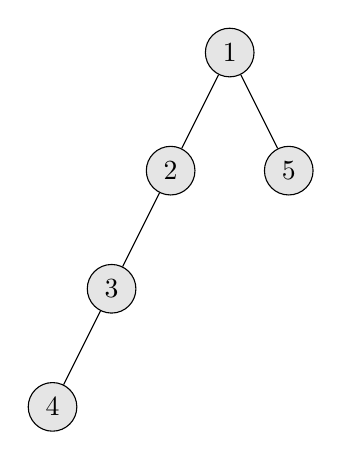
\begin{tikzpicture}
[every node/.style={draw, circle, fill=gray!20!, minimum size=5mm}]
\node{1}
child{node{2} child{ node{3} child{node{4}} child[missing] } child[missing]}
child{node{5}};
\end{tikzpicture}
\end{figure}
 
\textbf{Output}:
\begin{lstlisting}[style=customc, caption={}]
[["",  "",  "", "",  "", "", "", "1", "",  "",  "",  "",  "", "", ""]
 ["",  "",  "", "2", "", "", "", "",  "",  "",  "",  "5", "", "", ""]
 ["",  "3", "", "",  "", "", "", "",  "",  "",  "",  "",  "", "", ""]
 ["4", "",  "", "",  "", "", "", "",  "",  "",  "",  "",  "", "", ""]]d
\end{lstlisting}
\end{flushleft}

\textbf{Note}: 
\begin{itemize}
\item The height of binary tree is in the range of \lstinline[language=C++, basicstyle=\small\ttfamily, keywordstyle=\bfseries\color{green!40!black}]|[1, 10]|. 
\end{itemize}

\subsection{Divide And Conquer}
We need to get the height of the binary tree first, say $h$. The output matrix dimension will be $h\times (2^h-1)$. Then we go to the recursion process to put each node's value into the output matrix.
\begin{enumerate}
\item The recursive function will take current row, $r$, current size of columns $\ell$, and the start column $c$.
\item We put current node at the center of current row by considering the start column, i.e, $M[r][c + \ell/2]$.
\item Then we put left child of current node at next row with half of $l$, i.e, $M[r+1][c+\ell/4]$.
\item Next, we put right child of current node at next row with half of $l$ but the start column is $c+\ell/2+1$, i.e., $M[r+1][c+\ell/2+1+\ell/4]$
\item Go to step 1 to continue the recursive process. 
\end{enumerate}
% \section{656 --- Coin Path}
Given an array $A$ (index starts at 1) consisting of $N$ integers: $A_1$, $A_2$, $\ldots$, $A_N$ and an integer $B$. The integer $B$ denotes that from any place (suppose the index is $i$) in the array $A$, you can jump to any one of the place in the array A indexed $i+1$, $i+2$, $\ldots$ $i+B$ if this place can be jumped to. Also, if you step on the index $i$, you have to pay $A_i$ coins. If $A_i$ is $-1$, it means you can’t jump to the place indexed $i$ in the array.

Now, you start from the place indexed 1 in the array $A$, and your aim is to reach the place indexed $N$ using the minimum coins. You need to return the path of indexes (starting from 1 to $N$) in the array you should take to get to the place indexed $N$ using minimum coins.

If there are multiple paths with the same cost, return the lexicographically smallest such path.

If it's not possible to reach the place indexed $N$ then you need to return an empty array.

\paragraph{Example 1:}

\begin{flushleft}
\textbf{Input}: \lstinline[language=Java, basicstyle=\small\ttfamily, keywordstyle=\bfseries\color{green!40!black}]|[1,2,4,-1,2], 2|

\textbf{Output}: \lstinline[language=Java, basicstyle=\small\ttfamily, keywordstyle=\bfseries\color{green!40!black}]|[1,3,5]|

\end{flushleft}
 

\paragraph{Example 2:}

\begin{flushleft}
\textbf{Input}: \lstinline[language=Java, basicstyle=\small\ttfamily, keywordstyle=\bfseries\color{green!40!black}]|[1,2,4,-1,2], 1|

\textbf{Output}: \lstinline[language=Java, basicstyle=\small\ttfamily, keywordstyle=\bfseries\color{green!40!black}]|[]|

\end{flushleft}
 

\paragraph{Note:}

\begin{itemize}
\item Path $a_1, a_2, \ldots, a_n$ is lexicographically smaller than $b_1, b_2, \ldots, b_m$, if and only if at the first $i$ where $a_i$ and $b_i$ differ, $a_i < b_i$; when no such $i$ exists, then $n < m$.
\item $A_1 \geq 0$. $A_2, \ldots, A_N$ (if exist) will in the range of \lstinline[language=Java, basicstyle=\small\ttfamily, keywordstyle=\bfseries\color{green!40!black}]|[-1, 100]|.
\item Length of $A$ is in the range of \lstinline[language=Java, basicstyle=\small\ttfamily, keywordstyle=\bfseries\color{green!40!black}]|[1, 1000]|.
\item $B$ is in the range of \lstinline[language=Java, basicstyle=\small\ttfamily, keywordstyle=\bfseries\color{green!40!black}]|[1, 100]|.

\end{itemize}

\subsection{Backtrace}
This is a typical backtracking problem. We try each possible selection, and check if we can acheive the best result.

For this problem, we make use of an array $P$ with size $N$ to record next index of current index $i$, i.e, $P[i]$ is the next index from index $i$. At start, $P$ is filled  with all $-1$. 

In the backtracking process, With $i$ as the current index, we can consider every possible index from $i+1$ to $i+B$ as the next place to be jumped to. For every such next index, $j$, if this place can be jumped to, we determine the cost of reaching the end of the array, say $c$, which is starting from the index $i$, and with $j$ as the next index jumped from $i$. If $c$ is less than the global minimum cost, say $\kappa$, we can update $\kappa$ as $c$ and update $P[i]$ as $j$.

After the backtracking process finished, we traverse over the array $P$ starting from the index $0$. At every step, we add the current index to the result list and also move to the index pointed by $P[i]$, since this refers to the next index for the minimum cost.

\subsection{Backtracking With Memory}
In the brute force backtracking approach, a lot of duplicate function calls are made, since we are considering the same index through multiple paths. To remove this redundancy, we can make use of memorization.

We make use of an array, say $M$, to store the minimum cost of jumps to reach the end of the array $A$. Whenever the value for any index is calculated once, it is stored in its appropriate location. Thus, next time whenever the same function call is made, we can return the result directly from $M$, pruning the search space to a great extent.
% \section{657. Robot Return to Origin}
There is a robot starting at position \lstinline[language=C++, basicstyle=\small\ttfamily, keywordstyle=\bfseries\color{green!40!black}]|(0, 0)|, the origin, on a 2D plane. Given a sequence of its moves, judge if this robot \textbf{ends up at} \lstinline[language=C++, basicstyle=\small\ttfamily, keywordstyle=\bfseries\color{green!40!black}]|(0, 0)| after it completes its moves.

The move sequence is represented by a string, and the character \lstinline[language=C++, basicstyle=\small\ttfamily, keywordstyle=\bfseries\color{green!40!black}]|moves[i]| represents its $i$-th move. Valid moves are \lstinline[language=Java, basicstyle=\small\ttfamily, keywordstyle=\bfseries\color{green!40!black}]|R| (right), \lstinline[language=Java, basicstyle=\small\ttfamily, keywordstyle=\bfseries\color{green!40!black}]|L| (left), \lstinline[language=Java, basicstyle=\small\ttfamily, keywordstyle=\bfseries\color{green!40!black}]|U| (up), and \lstinline[language=Java, basicstyle=\small\ttfamily, keywordstyle=\bfseries\color{green!40!black}]|D| (down). If the robot returns to the origin after it finishes all of its moves, return \lstinline[language=C++, basicstyle=\small\ttfamily, keywordstyle=\bfseries\color{green!40!black}]|true|. Otherwise, return \lstinline[language=C++, basicstyle=\small\ttfamily, keywordstyle=\bfseries\color{green!40!black}]|false|.

\paragraph{Note:} 
\begin{itemize}
\item The way that the robot is \lstinline[language=Java, basicstyle=\small\ttfamily, keywordstyle=\bfseries\color{green!40!black}]|"facing"| is irrelevant. \lstinline[language=C++, basicstyle=\small\ttfamily, keywordstyle=\bfseries\color{green!40!black}]|"R"| will always make the robot move to the right once, \lstinline[language=C++, basicstyle=\small\ttfamily, keywordstyle=\bfseries\color{green!40!black}]|"L"| will always make it move left, etc. Also, assume that the magnitude of the robot's movement is the same for each move.

\end{itemize}

\paragraph{Example 1:}

\begin{flushleft}
\textbf{Input}: \lstinline[language=C++, basicstyle=\small\ttfamily, keywordstyle=\bfseries\color{green!40!black}]|"UD"|

\textbf{Output}: \lstinline[language=C++, basicstyle=\small\ttfamily, keywordstyle=\bfseries\color{green!40!black}]|true|

\textbf{Explanation}: The robot moves up once, and then down once. All moves have the same magnitude, so it ended up at the origin where it started. Therefore, we return \lstinline[language=C++, basicstyle=\small\ttfamily, keywordstyle=\bfseries\color{green!40!black}]|true|.

\end{flushleft}
 

\paragraph{Example 2:}

\begin{flushleft}
\textbf{Input}: \lstinline[language=C++, basicstyle=\small\ttfamily, keywordstyle=\bfseries\color{green!40!black}]|"LL"|

\textbf{Output}: \lstinline[language=C++, basicstyle=\small\ttfamily, keywordstyle=\bfseries\color{green!40!black}]|false|

\textbf{Explanation}: The robot moves left twice. It ends up two \lstinline[language=C++, basicstyle=\small\ttfamily, keywordstyle=\bfseries\color{green!40!black}]|"moves"| to the left of the origin. We return \lstinline[language=C++, basicstyle=\small\ttfamily, keywordstyle=\bfseries\color{green!40!black}]|false| because it is not at the origin at the end of its moves.
\end{flushleft}

\subsection{Simulation}
A very easy problem. Just simulate the coordinate changes for each direction.
% \section{658 --- Find K Closest Elements}
Given a sorted array, $A$, two integers $k$ and $x$, find the $k$ closest elements to $x$ in the array. The result should also be sorted in ascending order. If there is a tie, the smaller elements are always preferred.

\paragraph{Example 1:}

\begin{flushleft}
\textbf{Input}: \lstinline[language=C++, basicstyle=\small\ttfamily, keywordstyle=\bfseries\color{green!40!black}]|[1,2,3,4,5]|, $k=4$, $x=3$

\textbf{Output}: \lstinline[language=C++, basicstyle=\small\ttfamily, keywordstyle=\bfseries\color{green!40!black}]|[1,2,3,4]|
\end{flushleft}

\paragraph{Example 2:}

\begin{flushleft}
\textbf{Input}: \lstinline[language=C++, basicstyle=\small\ttfamily, keywordstyle=\bfseries\color{green!40!black}]|[1,2,3,4,5]|, $k=4$, $x=-1$

\textbf{Output}: \lstinline[language=C++, basicstyle=\small\ttfamily, keywordstyle=\bfseries\color{green!40!black}]|[1,2,3,4]|
\end{flushleft}

\paragraph{Note:}

\begin{itemize}
\item The value $k$ is positive and will always be smaller than the length of the sorted array.
\item Length of the given array is positive and will not exceed $10^4$
\item Absolute value of elements in the array and $x$ will not exceed $10^4$
\end{itemize}

\subsection{Binary Search} 
Since the given array is sorted, we can make use of binary search to find the start index of the these $k$ closest elements.

If current midpoint index is $m$, we need to determine whether we will search in upper half or lower half range based on some condition.

The condition is given by comparing $x - A[m]$ and $A[m+k] - x$.

\begin{itemize}
\item If $x-A[m] > A[m+k] - x$, this means $k$ elements from $A[m+1, m+k]$ closer to $x$ than those from $A[m, m+k-1]$. The reason is that $A[m+1, m+k]$ and $A[m, m+k-1]$ share $k-1$ same elements that are $A[m+1,m+k-1]$, the only difference is $A[m]$ and $A[m+k]$. In this case, we will search in the upper half, i.e., $l\gets m+1$.
\item Otherwise, based on the same reasoning, we will search in the lower half, i.e., $r\gets mid$. (Leftmost binary search)
\end{itemize}

Notice that we do not use the absolute value of $x-A[m]$ and $A[m+k]-x$ to compare. For example, when $A[m+k]< x$, we may try next in the upper half range. If we compare based on absolute value, it may still try next in the lower half range, and we will get larger gap to $x$.


% \section{659 --- Split Array into Consecutive Subsequences}
Given an array \fcj{nums} sorted in ascending order, return \fcc{true} if and only if you can split it into 1 or more subsequences such that each subsequence consists of consecutive integers and has length at least 3.

\paragraph{Example 1:}

\begin{flushleft}
\textbf{Input}: \fcj{[1,2,3,3,4,5]}

\textbf{Output}: \fcc{true}

\textbf{Explanation}:

You can split them into two consecutive subsequences:
 
1, 2, 3

3, 4, 5
\end{flushleft}

\paragraph{Example 2:}

\begin{flushleft}
\textbf{Input}: \fcj{[1,2,3,3,4,4,5,5]}

\textbf{Output}: \fcc{true}

\textbf{Explanation}:

You can split them into two consecutive subsequences : 

1, 2, 3, 4, 5

3, 4, 5

\end{flushleft}

\paragraph{Example 3:}

\begin{flushleft}
\textbf{Input}: \fcj{[1,2,3,4,4,5]}


\textbf{Output}: \fcc{false}
\end{flushleft}

 

\paragraph{Constraints:}

\begin{itemize}
\item  $ 1 \leq \lvert A\rvert \leq 10000$
\end{itemize}

\subsection{Greedy}
The basic idea is that, for each distinct element $x$ in the input array, we only need to maintain three variables, i.e., the number of consecutive sub-sequences ending at $x$ with length of 1, 2 and larger than 2.

Suppose $x$ is the current number we are processing, and the count of $x$ is $\Delta_x$. We also assume $t$ is the number we have processed immediately before $x$.

We denote the the number of consecutive sub-sequences ending at $t0$ with length 1, 2 and larger than 2 are $\ell_1$, $\ell_2$ and $\ell_3$ respectively.

Then, we have two scenarios:

$\star$  When $x\neq t+1$: in this case, we cannot add $x$ to any consecutive subsequence ending at $t$. Thus $\ell_1=\ell_2=0$ (i.e., the consecutive sequence ending at $t$ with length 1 and 2).
 
Suppose $l_1$, $l_2$ and $l_3$ are number of consecutive sub-sequences ending at $x$ with length 1, 2 and no less than 3, we will have $l_1=\Delta_x$, $l_2=0$ and $l_3=0$, which means we only have $\Delta_x$ consecutive subsequence with length 1 ending at $x$.

$\star$ When $x=t+1$. This allows us to add $x$ to consecutive sub-sequences ending at $t$ and thus extend those sub-sequences.

But we should add these $x$ to those sub-sequences with length 1 first, and length 2 secondly, and finally to those with length larger than 2. We also need $\Delta_x\geq \ell_1+\ell_2$. If this condition is violated, some consecutive sequences will extend length over 2.

As in first case, we use $l_1$, $l_2$ and $l_3$ to represent the number of consecutive sub-sequences ending at $x$ with length of 1, 2 and over 2 respectively. We can get following relationships
\begin{align*}
    l_2 &= \ell_1 \\
    l_3 &= \ell_2 + \min(\ell_3, \Delta_x-(\ell_1+\ell_2)) \\
   l_1 &= \max(\Delta_x - (\ell_1+\ell_2+\ell_3), 0)
\end{align*}

Since we add $x$ to the consecutive sub-sequence ending at $t$ with length 1 firstly, the consecutive sub-sequence ending $x$ will have length 2. Thus, $l_2 \gets \ell_1$.

Next, we add remaining $x$ to those consecutive sub-sequences ending at $t$ with length 2. These will give consecutive sub-sequences ending at $x$ with length 3. Thus, $l_3\geq \ell_2$. If $\Delta_x > \ell_1 + \ell_2$, we still have some $x$ to use and can add them to the subsequences ending at $t$ with length over 2. All these subsequences ending at $t$ have length over 2, and the total number of such subsequences is $\ell_2 + \min(\ell_3, \Delta_x - (\ell_1 + \ell_2))$. 

If $\Delta_x > \ell_1 + \ell_2 + \ell_3$, we still have remaining $x$s will form the sub-sequences ending at $x$ with length 1, and thus $l_1 = \max(\Delta_x - (\ell_1 + \ell_2 + \ell_3), 0)$.

Finally, if we get $\ell_1=0$ and $\ell_2=0$, we can split the array into consecutive parts. Otherwise, it cannot be done.

\setcounter{lstlisting}{0}
\begin{lstlisting}[style=customc, caption={Greedy}]
bool isPossible( vector<int>& nums )
{
    //number of subsequence with length 1 ending at x
    long long l1{};
    //number of subsequence with length 2 ending at x
    long long l2{};
    //number of subsequence with length over 2 ending at x
    long long l3{};
    //previous element visited
    int prev{};
    for( auto s = begin( nums ); s != end( nums ); )
    {
        int x = *s;
        auto next_s = upper_bound( s, end( nums ), x );
        auto count_x = distance( s, next_s );
        if( s == begin( nums ) )
        {
            //we have count_x subsequence with length 1
            //which are ending at x
            l1 = count_x;
            s = next_s;
            prev = x;
            continue;
        }
        if( x != prev + 1 )
        {
            //x cannot be added to subsequence ending at prev
            if( ( l1 > 0 ) || ( l2 > 0 ) )
            {
                //we only have subsequence with length 1 or 2
                //ending at prev
                //Thus we cannot get conseuctive part with length >= 3
                return false;
            }
            //subsequence with length 1 ending at x
            l1 = count_x;
            //subsequence with length 2 ending at x
            l2 = 0;
            //subsequence with length over 2 ending at x
            l3 = 0;
        }
        else
        {
            if( count_x < l1 + l2 )
            {
                //We don't have enough x to add to
                //subsequence with length 1 and 2 ending at prev
                //which will leave some subsequence ending at prev
                //with length less than 3
                return false;
            }
            //x can be added to subsequence ending at prev
            //add to subsequence with length 1 ending at prev first
            //Thus we have
            auto cur_l2 = l1;
            //then add to subsequence with length 2 ending at prev
            auto cur_l3 = l2;
            //if there still some x left
            //we can extend subsequence with length 3 ending at prev
            if( count_x > l1 + l2 )
            {
                //we can only extend to minimum of l3 and count_x - l1 - l2
                //subsequences with length over 3
                cur_l3 += ( min )( l3, count_x - l1 - l2 );
            }
            //If we still have some x left,
            //these x will form a subsequence with length 1 ending at x
            auto cur_l1 = ( max )( 0ll, count_x - l1 - l2 - l3 );

            //update to l1, l2 and l3
            l1 = cur_l1;
            l2 = cur_l2;
            l3 = cur_l3;
        }

        s = next_s;
        prev = x;
    }
    if( ( l1 == 0 ) && ( l2 == 0 ) )
    {
        //we don't have subsequence with length less than 3
        //ending at last element in the given array
        return true;
    }
    return false;
}
\end{lstlisting}

\subsection{Greedy With Two Pass}
In first pass we get the counts of each number.

During the second pass, make use of another hash map to record the number of consecutive subsequences with length over 2 found so far.

For each number $i$, we try to put it to the tail of one of found subsequence ending at $i-1$. 

If we cannot, we may use $i+1$ and $i+2$ along with $i$ to generate a new subsequence. 

\begin{lstlisting}[style=customc, caption={Two Pass}]
bool isPossible( vector<int>& nums )
{
    unordered_map<int, int> counts;
    unordered_map<int, int> need;
    for( int n : nums )
    {
        counts[n] += 1;
    }
    for( int n : nums )
    {
        auto it = counts.find( n );
        if( it->second == 0 )
        {
            //skip n, since no subsequence
            //can be formed
            continue;
        }
        auto p = need.find( n );
        if( ( p != need.end() ) && ( p->second > 0 ) )
        {
            //consume n
            p->second -= 1;
            //we need another n+1
            need[n + 1] += 1;
        }
        else if( auto c1 = counts.find( n + 1 ), c2 = counts.find( n + 2 );
                 ( ( c1 != counts.end() ) && ( c1->second > 0 ) && ( c2 != counts.end() ) && ( c2->second > 0 ) ) )
        {
            //we consume n+1 and n+2
            --c1->second;
            --c2->second;
            //we need another n+3
            need[n + 3] += 1;
        }
        else
        {
            return false;
        }
        --it->second;
    }
    return true;
}
\end{lstlisting}
% \section{660 --- Remove 9}
Start from integer 1, remove any integer that contains 9 such as 9, 19, 29.

So now, you will have a new integer sequence: $1, 2, 3, 4, 5, 6, 7, 8, 10, 11, \ldots$

Given a positive integer $n$, you need to return the $n$-th integer after removing. Note that 1 will be the first integer.

\paragraph{Example 1:}
\begin{flushleft}
\textbf{Input}: 9

\textbf{Output}: 10
\end{flushleft}

\paragraph{Hint:}
\begin{itemize}
    \item $n$ will not exceed $9 \times 10^8$.
\end{itemize}

\subsection{Mathematical}
Let's write the first numbers and try to notice a pattern. Those numbers are:
\begin{align*}
& 1, 2, 3, 4, 5, 6, 7, 8, \\
& 10, 11, 12, 13, 14, 15, 16, 17, 18,\\
& 20, 21, 22, 23, 24, 25, 26, 27, 28, \ldots \\
& 80, 81, 82, 83, 84, 85, 86, 87, 88, \\
& 100, 101, 102, \ldots
\end{align*}

These numbers look exactly like all base-9 numbers!

Indeed, every base-9 number is a number in this sequence, and every number in this sequence is a base-9 number. Both this sequence and the sequence of all base-9 numbers are in increasing order. The answer is therefore just the $n$-th base-9 number.



% \section{661 --- Image Smoother}
Given a 2D integer matrix $M$ representing the gray scale of an image, you need to design a smoother to make the gray scale of each cell becomes the average gray scale (rounding down) of all the 8 surrounding cells and itself. If a cell has less than 8 surrounding cells, then use as many as you can.

\paragraph{Example 1:}
\begin{flushleft}

\textbf{Input}:

\[
\begin{Bmatrix}
1 & 1 & 1\\
1 & 0 & 1\\
1 & 1 & 1
\end{Bmatrix}
\]

\textbf{Output}:

\[
\begin{Bmatrix}
0 & 0 & 0\\
0 & 0 & 0\\
0 & 0 & 0
\end{Bmatrix}
\]

\textbf{Explanation}:

For the point \lstinline[language=Java, basicstyle=\small\ttfamily, keywordstyle=\bfseries\color{green!40!black}]|(0,0), (0,2), (2,0), (2,2)|: $\lfloor3/4\rfloor = \lfloor0.75\rfloor = 0$

For the point \lstinline[language=Java, basicstyle=\small\ttfamily, keywordstyle=\bfseries\color{green!40!black}]|(0,1), (1,0), (1,2), (2,1)|: $\lfloor5/6\rfloor = \lfloor0.83333333\rfloor = 0$

For the point \lstinline[language=Java, basicstyle=\small\ttfamily, keywordstyle=\bfseries\color{green!40!black}]|(1,1)|: $\lfloor 8/9 \rfloor = \lfloor 0.88888889\rfloor = 0$

\end{flushleft}

\paragraph{Note:}
\begin{itemize}
\item The value in the given matrix is in the range of \lstinline[language=Java, basicstyle=\small\ttfamily, keywordstyle=\bfseries\color{green!40!black}]|[0, 255]|.
\item The length and width of the given matrix are in the range of \lstinline[language=Java, basicstyle=\small\ttfamily, keywordstyle=\bfseries\color{green!40!black}]|[1, 150]|.
\end{itemize}

\subsection{Encode Average Value}
Since each pixel in the image has value in \lstinline[language=Java, basicstyle=\small\ttfamily, keywordstyle=\bfseries\color{green!40!black}]|[0, 255]|, we can use the additional bits to record the average value for current pixel. For example, we may use bit 15 to bit 8 to save the average value.

After getting all the average values, we will iterate the image again to get the average value for each pixel.

% \section{662 --- Maximum Width of Binary Tree}
Given a binary tree, write a function to get the maximum width of the given tree. The width of a tree is the maximum width among all levels. The binary tree has the same structure as a full binary tree, but some nodes are null.

The width of one level is defined as the length between the end-nodes (the leftmost and right most non-null nodes in the level, where the null nodes between the end-nodes are also counted into the length calculation.

\paragraph{Example 1:}

\begin{flushleft}
\textbf{Input}:

\begin{figure}[H]
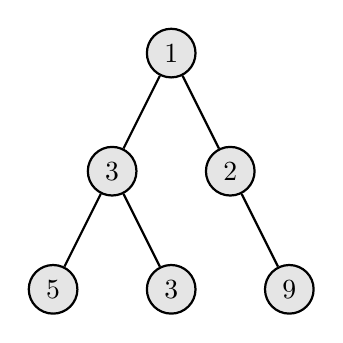
\begin{tikzpicture}
[every node/.style={draw, circle,
 minimum size=6mm, fill=gray!20!},
  node distance=8mm, 
  every join/.style={>=stealth,->},
 thick
]
\node{1}
child{node{3} child{node{5}} child{node{3}} }
child{node{2} child[missing] child{node{9}}};
\end{tikzpicture}
\end{figure} 

\textbf{Output}: 4

\textbf{Explanation}: The maximum width existing in the third level with the length 4  \lstinline[language=Java, basicstyle=\small\ttfamily, keywordstyle=\bfseries\color{green!40!black}]|(5,3,null,9)|.
\end{flushleft}

\paragraph{Example 2:}

\begin{flushleft}
\textbf{Input}: 

\begin{figure}[H]
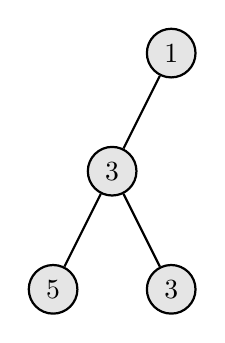
\begin{tikzpicture}
[every node/.style={draw, circle,
 minimum size=6mm, fill=gray!20!},
  node distance=8mm, 
  every join/.style={>=stealth,->},
 thick
]
\node{1}
child{node{3} child{node{5}} child{node{3}}}
child[missing];
\end{tikzpicture}
\end{figure}

\textbf{Output}: 2

\textbf{Explanation}: 

The maximum width existing in the third level with the length 2 (5,3).
\end{flushleft}

\paragraph{Example 3:}
\begin{flushleft}


\textbf{Input}: 

\begin{figure}[H]
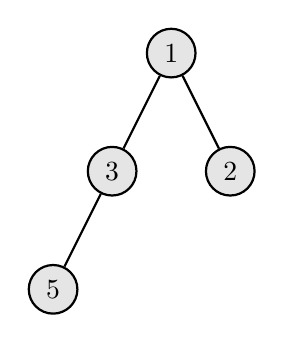
\begin{tikzpicture}
[every node/.style={draw, circle,
 minimum size=6mm, fill=gray!20!},
  node distance=8mm, 
  every join/.style={>=stealth,->},
 thick
]
\node{1}
child{node{3} child{node{5}} child[missing]}
child{node{2}};
\end{tikzpicture}
\end{figure}


\textbf{Output}: 2

\textbf{Explanation}: 

The maximum width existing in the second level with the length 2  \lstinline[language=Java, basicstyle=\small\ttfamily, keywordstyle=\bfseries\color{green!40!black}]|(3,2)|.
\end{flushleft}

\paragraph{Example 4:}

\begin{flushleft}


\textbf{Input}: 

\begin{figure}[H]
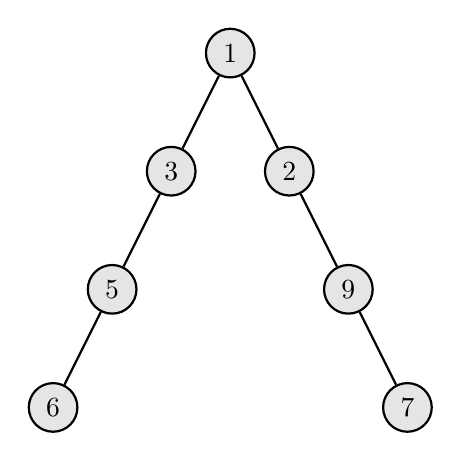
\begin{tikzpicture}
[every node/.style={draw, circle, minimum size=6mm, fill=gray!20!},
  node distance=8mm, 
  every join/.style={>=stealth,->},
 thick
]
\node{1}
child{node{3} child{node{5} child{node{6}} child[missing] } child[missing] }
child{node{2} child[missing] child{node{9} child[missing] child{node{7}} }  };
\end{tikzpicture}
\end{figure}
    
\textbf{Output}: 8

\textbf{Explanation}:

The maximum width existing in the fourth level with the length 8 

 \lstinline[language=Java, basicstyle=\small\ttfamily, keywordstyle=\bfseries\color{green!40!black}]|(6,null,null,null,null,null,null,7)|.
\end{flushleft}

\paragraph{Note:} 

\begin{itemize}
\item Answer will in the range of 32-bit signed integer.
\end{itemize}

\subsection{Breadth First Search}
We can assign each node a id. For example, the root node's id is zero and its left/right child's is 1 or 2 respectively. Specifically, if a node has a id $n$, the left and right child ids are $2n+1$ and $2n+2$ respectively.

On each level, get the first node's id $x$ and the last node's id $y$. The width is then $y-x+1$.

In C++ implementation, we may need  \lstinline[language=C++, basicstyle=\small\ttfamily, keywordstyle=\bfseries\color{green!40!black}]|unsigned long| as the type for id. It will fix the overflow for one test case.
% \section{663 --- Equal Tree Partition}
Given a binary tree with n nodes, your task is to check if it's possible to partition the tree to two trees which have the equal sum of values after removing exactly one edge on the original tree.

\paragraph{Example 1:}

\begin{flushleft}
\textbf{Input}:     

\begin{figure}[H]
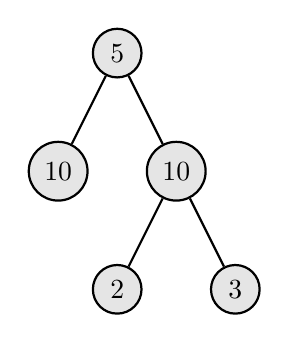
\begin{tikzpicture}
[every node/.style={draw, circle,
 minimum size=6mm, fill=gray!20!},
  node distance=8mm, 
  every join/.style={>=stealth,->},
 thick
]
\node{5}
child{node{10}}
child{node{10} child{node{2}} child{node{3}} };
\end{tikzpicture}
\end{figure}

\textbf{Output}:  \lstinline[language=C++, basicstyle=\small\ttfamily, keywordstyle=\bfseries\color{green!40!black}]|true|

\textbf{Explanation}: 

\begin{figure}[H]
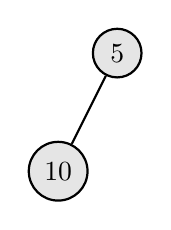
\begin{tikzpicture}
[every node/.style={draw, circle,
 minimum size=6mm, fill=gray!20!},
  node distance=8mm, 
  every join/.style={>=stealth,->},
 thick
]
\node{5}
child{node{10}}
child[missing];
\end{tikzpicture}
\end{figure}
    
Sum: 15

\begin{figure}[H]
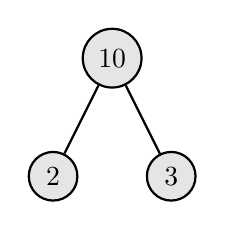
\begin{tikzpicture}
[every node/.style={draw, circle,
 minimum size=6mm, fill=gray!20!},
  node distance=8mm, 
  every join/.style={>=stealth,->},
 thick
]
\node{10}
child{node{2}}
child{node{3}};
\end{tikzpicture}
\end{figure}

Sum: 15
\end{flushleft}

\paragraph{Example 2:}
\begin{flushleft}


\textbf{Input}:     
\begin{figure}[H]
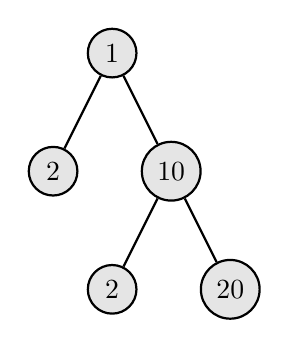
\begin{tikzpicture}
[every node/.style={draw, circle,
 minimum size=6mm, fill=gray!20!},
  node distance=8mm, 
  every join/.style={>=stealth,->},
 thick
]
\node{1}
child{node{2}}
child{node{10} child{node{2}} child{node{20}} };
\end{tikzpicture}
\end{figure}

\textbf{Output}:  \lstinline[language=C++, basicstyle=\small\ttfamily, keywordstyle=\bfseries\color{green!40!black}]|false|

\textbf{Explanation}: 

You can't split the tree into two trees with equal sum after removing exactly one edge on the tree.
\end{flushleft}

\paragraph{Note:}

\begin{itemize}
\item The range of tree node value is in the range of  \lstinline[language=C++, basicstyle=\small\ttfamily, keywordstyle=\bfseries\color{green!40!black}]|[-100000, 100000]|.
\item $1 \leq n \leq 10000$
\end{itemize}

\subsection{Depth First Search}
After removing a edge from parent to child, the subtree rooted at child must be half the sum of the entire tree.

We can put the sum of every subtree into an array by depth-first search. Then, we check if we can find a value inside the array which is half the sum of the entire tree.

In the implementation, we should pay attention to a few notes
\begin{itemize}
\item The sum of a subtree rooted at current node will be the current last element of the array.
\item The total sum of entire tree should be even number.
\item We need to remove last element of the array which is the total sum of entire tree. 
\end{itemize}

% \section{664 --- Strange Printer}
There is a strange printer with the following two special requirements:

\begin{enumerate}
\item The printer can only print a sequence of the same character each time.
\item At each turn, the printer can print new characters starting from and ending at any places, and will cover the original existing characters.
\end{enumerate}

Given a string consists of lower English letters only, your job is to count the minimum number of turns the printer needed in order to print it.

\paragraph{Example 1:}

\begin{flushleft}


\textbf{Input}:  \lstinline[language=C++, basicstyle=\small\ttfamily, keywordstyle=\bfseries\color{green!40!black}]|"aaabbb"|

\textbf{Output}: 2

\textbf{Explanation}: Print  \lstinline[language=C++, basicstyle=\small\ttfamily, keywordstyle=\bfseries\color{green!40!black}]|"aaa"| first and then print  \lstinline[language=C++, basicstyle=\small\ttfamily, keywordstyle=\bfseries\color{green!40!black}]|"bbb"|.

\end{flushleft}

\paragraph{Example 2:}

\begin{flushleft}

\textbf{Input}:  \lstinline[language=C++, basicstyle=\small\ttfamily, keywordstyle=\bfseries\color{green!40!black}]|"aba"|

\textbf{Output}: 2

\textbf{Explanation}: Print  \lstinline[language=C++, basicstyle=\small\ttfamily, keywordstyle=\bfseries\color{green!40!black}]|"aaa"| first and then print  \lstinline[language=C++, basicstyle=\small\ttfamily, keywordstyle=\bfseries\color{green!40!black}]|"b"| from the second place of the string, which will cover the existing character  \lstinline[language=C++, basicstyle=\small\ttfamily, keywordstyle=\bfseries\color{green!40!black}]|'a'|.

\end{flushleft}

\paragraph{Hint:} 
\begin{itemize}
\item Length of the given string will not exceed 100.
\end{itemize}

\subsection{Dynamic Programming}
Suppose $F[i][j]$ is the minimum number of turns the printers needs in order to print $S[i, j]$. 

The base cases are direct

\begin{enumerate}
\item $i=j$: $F[i][i]:=1$
\item $j=i+1$: $F[i][i+1]$ depends on if $S[i]=S[i+1]$.When $S[i]=S[i+1]$, $F[i][i+1]:=1$. Otherwise, $F[i][i+1]:=2$.
\end{enumerate}

Next, we iterate the sub-string length from $3$ to $\ell$. $\ell$ is the length of $s$. For any sub-string $S[i,j]$, the initial value of $F[i][j]$ can be set to $1+F[i+1][j]$ since we can print $S[i]$ first and then print $s[i+1,j]$.

Then, we check each index $k$ from $i+1$ to $j$. The total turns for printing $s[i,j]$ will be $F[i,k-1]+F[k, j]$. However, if $s[i]=s[k]$, we don't need to print $s[k]$ separately. We can print $s[i]$ with $s[k]$ in one turn. Thus the total turns can be decreased by one time, i.e. $F[i,k-1]+F[k, j]-1$.

We choose the minimum turns from above as the result for $F[i][j]$. Finally, $F[0][\ell-1]$ gives the result for $s$.
% \section{665 --- Non-decreasing Array}
Given an array with $n$ integers, your task is to check if it could become non-decreasing by modifying at most 1 element.

We define an array, $A$, is non-decreasing if $A[i] \leq A[i + 1]$ holds for every $i$ ($1 \leq i < n$).

\paragraph{Example 1:}

\begin{flushleft}

\textbf{Input}: \lstinline[language=C++, basicstyle=\small\ttfamily, keywordstyle=\bfseries\color{green!40!black}]|[4,2,3]|

\textbf{Output}: \lstinline[language=C++, basicstyle=\small\ttfamily, keywordstyle=\bfseries\color{green!40!black}]|true|

\textbf{Explanation}: You could modify the first 4 to 1 to get a non-decreasing array.

\end{flushleft}

\paragraph{Example 2:}

\begin{flushleft}

\textbf{Input}: \lstinline[language=C++, basicstyle=\small\ttfamily, keywordstyle=\bfseries\color{green!40!black}]|[4,2,1]|

\textbf{Output}: \lstinline[language=C++, basicstyle=\small\ttfamily, keywordstyle=\bfseries\color{green!40!black}]|false|

\textbf{Explanation}: You can't get a non-decreasing array by modify at most one element.

\end{flushleft}


\paragraph{Note:} 

\begin{itemize}
\item The $n$ belongs to \lstinline[language=C++, basicstyle=\small\ttfamily, keywordstyle=\bfseries\color{green!40!black}]|[1, 10,000]|. 
\end{itemize}

\subsection{Analyze Index}
\begin{itemize}
\item 如果找到两个位置出现 $A[i] > A[i+1]$, 很显然是不能做到的。返回\texttt{false}。
\item 假设在唯一的位置$P$出现$A[P] > A[P+1]$。
\begin{enumerate}
\item 如果$P=0$,把$A[0]$换成任何一个小于$A[1]$的数即可。
\item 如果$P=L-2$,把$A[L-1]$换成$A[L-2]$即可。有没有可能$A[L-3]$大于$A[L-1]$呢?即使出现这种情况,由于我们已经把$A[L-1]$替换为$A[L-2]$了,那么替换后$A[L-1] \geq A[L-3]$。至于$A[L-3]$之前有没有可能大于$A[L-1]$,就没必要分析了,因为这些数必然小于$A[L-3]$,因为$P$是唯一出现$A[P] > A[P+1]$的位置。
\end{enumerate}
\item 如果$P$不是上述两个边界位置,那么需要考虑$A[P-1]$, $A[P]$, $A[P+1]$以及$A[P+2]$这四个 number。这四个的关系是$A[P-1] \leq A[P] > A[P+1] \leq A[P+2]$
\begin{enumerate}
\item 如果$A[P-1] > A[P+1]$,$A[P-1]$之前的就不用分析了,因为都不大于$A[P-1]$。如果将$A[P+1]$修改为$A[P]$就可以使得$A[P-1] \leq A[P+1]$了,因为$A[P-1]\leq A[P]$。这时候四个数关系变为$A[P-1] \leq A[P] = A[P+1] ? A[P+2]$。因为$A[P+1] \gets A[P]$,所以$A[P+1]$与 $A[P+2]$的大小关系未知,如果需要满足题目要求最多改动一个位置,那么必然要求$A[P] \leq A[P+2]$。
\item 如果$A[P] > A[P+2]$,那么需要把$A[P]$换成$A[P+1]$,这样就有$A[P-1] ? A[P] = A[P+1] \leq A[P+2]$,因为$A[P] \gets A[P+1]$, 所以$A[P-1]$与 $A[P]$的大小关系未知。,如果需要满足题目要求最多改动一个位置,那么必然要求$A[P-1] \leq A[P+1]$
\end{enumerate}
\item 综合以上分析,可以得出结论,如果$A[P-1] > A[P+1]$ 并且 $A[P] > A[P+2]$,肯定不能只移动一个位置,反之,则是可以的
\end{itemize}
% \section{666 --- Path Sum IV}
If the depth of a tree is smaller than \textcolor{red}{5}, then this tree can be represented by a list of three-digits integers.

For each integer in this list:

\begin{enumerate}
\item The hundreds digit represents the depth $D$ of this node, $1 \leq D \leq 4$.
\item The tens digit represents the position $P$ of this node in the level it belongs to, $1 \leq P \leq 8$. The position is the same as that in a full binary tree.
\item The units digit represents the value $V$ of this node, $0 \leq V \leq 9$.

\end{enumerate}
 

Given a list of ascending three-digits integers representing a binary tree with the depth smaller than 5, you need to return the sum of all paths from the root towards the leaves.

\paragraph{Example 1:}

\begin{flushleft}
\textbf{Input}: \lstinline[language=C++, basicstyle=\small\ttfamily, keywordstyle=\bfseries\color{green!40!black}]|[113, 215, 221]|

\textbf{Output}: 12

\textbf{Explanation}: 

The tree that the list represents is:

\begin{figure}[H]
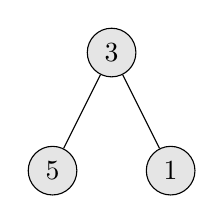
\begin{tikzpicture}
[every node/.style={draw, circle, fill=gray!20!, minimum size=5mm}]
\node{3}
child{node{5}}
child{node{1}};
\end{tikzpicture}
\end{figure}

The path sum is $(3 + 5) + (3 + 1) = 12$.
\end{flushleft}

 

\paragraph{Example 2:}

\begin{flushleft}
\textbf{Input}: \lstinline[language=C++, basicstyle=\small\ttfamily, keywordstyle=\bfseries\color{green!40!black}]|[113, 221]|

\textbf{Output}: 4

\textbf{Explanation}: 

The tree that the list represents is: 

\begin{figure}[H]
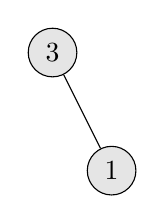
\begin{tikzpicture}
[every node/.style={draw, circle, fill=gray!20!, minimum size=5mm}]
\node{3}
child[missing]
child{node{1}};
\end{tikzpicture}
\end{figure}

The path sum is $(3 + 1) = 4$.
\end{flushleft}

\subsection{Breadth First Search}
For a full binary tree, at level $x$, there will be $2^{x-1}$ nodes.

\subsection{Breadth First Search}
For a full binary tree, at level $x$, there will be $2^{x-1}$ nodes.

\begin{enumerate}
\item Get the maximum level, say $Y$, by parsing the last element of input array $A$.
\item Iterate from level 1 to $Y$. At each level $x$
\begin{itemize}
\item Create an array, say $T$,  with size $2^{x-1}$ to save each node's accumulated sum from its parent node. 
\item If a node's position in current level is $P$, we can get its parent's index by $(P-1)/2$ since $P$ is starting with 1.
\item Add the value of its parent node to this node's own value and save to $T[P-1]$ since $P$ is starting with 1.
\item To avoid neglecting those nodes that don't have child nodes when processing next level (since we are swap $T$ to last level array), we put indices of the parent nodes with children into a hash set $S$. 
\item After complete processing whole nodes in current level, we accumulate the values of parent nodes without children into $z$ which is used to maintain the sum of those nodes without children. This is done by checking if a parent node's index is in the hash set $S$ or not.
\item Swap $T$ with another array, say $U$, which represents parent nodes.
\end{itemize}
\item Finally, we summation all the values of $U$ which contains the last level's nodes, and plus $z$.
\end{enumerate}

% \section{667 --- Beautiful Arrangement II}
Given two integers $n$ and $k$, you need to construct a list which contains $n$ different positive integers ranging from 1 to $n$ and obeys the following requirement:

Suppose this list is $[a_1, a_2, a_3, \ldots , a_n]$, then the list $[\lvert a_1 - a_2\rvert, \lvert a_2 - a_3\rvert, \lvert a_3 - a_4\rvert, \ldots , \lvert a_{n-1} - a_n\rvert]$ has exactly k distinct integers.

If there are multiple answers, print any of them.

\paragraph{Example 1:}

\begin{flushleft}
\textbf{Input}: $n = 3$, $k = 1$

\textbf{Output}: \lstinline[language=C++, basicstyle=\small\ttfamily, keywordstyle=\bfseries\color{green!40!black}]|[1, 2, 3]|

\textbf{Explanation}: The \lstinline[language=C++, basicstyle=\small\ttfamily, keywordstyle=\bfseries\color{green!40!black}]|[1, 2, 3]| has three different positive integers ranging from 1 to 3, and the \lstinline[language=C++, basicstyle=\small\ttfamily, keywordstyle=\bfseries\color{green!40!black}]|[1, 1]| has exactly 1 distinct integer: 1.
\end{flushleft}

\paragraph{Example 2:}

\begin{flushleft}
\textbf{Input}: $n = 3$, $k = 2$

\textbf{Output}: \lstinline[language=C++, basicstyle=\small\ttfamily, keywordstyle=\bfseries\color{green!40!black}]|[1, 3, 2]|

\textbf{Explanation}: The \lstinline[language=C++, basicstyle=\small\ttfamily, keywordstyle=\bfseries\color{green!40!black}]|[1, 3, 2]| has three different positive integers ranging from 1 to 3, and the \lstinline[language=C++, basicstyle=\small\ttfamily, keywordstyle=\bfseries\color{green!40!black}]|[2, 1]| has exactly 2 distinct integers: 1 and 2.
\end{flushleft}

\paragraph{Note:}
\begin{itemize}
\item The $n$ and $k$ are in the range $1 \leq k < n \leq 10^4$.
\end{itemize}

\subsection{Simulation}
We can construct the array by the following approach:

\begin{itemize}
\item $A[0] = 1$, $A[1] = k+A[0]$, $A[2] = A[1] - (k-1) = 2$, $A[3] = A[2] + (k-2)$, $\ldots, A[k] = A[k-1] + 1$
\item 观察以上规律,数字之间的间隔$D$以如下方式出现
\[
k,\quad -(k-1), \quad (k-2), \quad \ldots, \quad (-1)^{i}(k-i), \quad \dots, \quad 1
\]
\item 因为数字是$1\to n$,有$n-1$个间隔,所以如果 $K > n-1$肯定是不行的。 
\item After the above arrangement, we put $k+1$ numbers into the range $A[0, k]$. These numbers are from 1 to $k+1$. We need to arrange the remaining numbers which are from $k+2$ to $n$ into the range $A[k+1,n-1]$. These can be easily done by set $A[x]=x+1$ where $x\in [k+1, n-1]$.
\end{itemize}


% \section{668 --- Kth Smallest Number in Multiplication Table}
Nearly every one have used the Multiplication Table. But could you find out the $k$-th smallest number quickly from the multiplication table?

Given the height $m$ and the length $n$ of a $m \times n$ Multiplication Table, and a positive integer $k$, you need to return the $k$-th smallest number in this table.

\paragraph{Example 1:}

\begin{flushleft}

\textbf{Input}: $m = 3$, $n = 3$, $k = 5$

\textbf{Output}: 3

\textbf{Explanation}: 

The Multiplication Table:
\[
\begin{bmatrix}
1 & 2 & 3 \\
2 & 4 & 6 \\
3 & 6 & 9
\end{bmatrix}
\]

The 5-th smallest number is 3 \lstinline[language=C++, basicstyle=\small\ttfamily, keywordstyle=\bfseries\color{green!40!black}]|(1, 2, 2, 3, 3)|.

\end{flushleft}

\paragraph{Example 2:}

\begin{flushleft}

\textbf{Input}: $m = 2$, $n = 3$, $k = 6$

\textbf{Output}: 6

\textbf{Explanation}: 

The Multiplication Table:

\[
\begin{bmatrix}
1 & 2 & 3 \\
2 & 4 & 6
\end{bmatrix}
\]
The 6-th smallest number is 6 \lstinline[language=C++, basicstyle=\small\ttfamily, keywordstyle=\bfseries\color{green!40!black}]|(1, 2, 2, 3, 4, 6)|.

\end{flushleft}

\paragraph{Note:}

\begin{itemize}
\item The $m$ and $n$ will be in the range \lstinline[language=C++, basicstyle=\small\ttfamily, keywordstyle=\bfseries\color{green!40!black}]|[1, 30000]|.
\item The $k$ will be in the range $[1, m\times n]$.
\end{itemize}

\subsection{Binary Search}
$m \times n$的乘法表中,最小的数为\textbf{1}, 最大的数为$m\times n$.
\begin{itemize}
\item 对于每个候选值,在乘法表中寻找不大于该数的数有多少个,如果个数小于$k$,就跳到后半区,否则在前半区。
\item 在乘法表中,行$i$的最大数为$ i \times n$。所以在这行中,小于目标数$T$的个数为$ T / i$,但是由于有$n$的限制,所以应该取较小的那个,也就是$\min(T/i, n)$。
\item To count how many numbers are no larger than the target number, we iterate from 1 to $m$, and accumulate $\min(T/i, n)$ for row $i$.
\item 这里使用的二分法查找采用的是找\textbf{leftmost}的算法。
\end{itemize}
% \section{669 --- Trim a Binary Search Tree}
Given a binary search tree and the lowest and highest boundaries as $L$ and $R$, trim the tree so that all its elements lies in $[L, R]$ ($R \geq L$). You might need to change the root of the tree, so the result should return the new root of the trimmed binary search tree.

\paragraph{Example 1:}

\begin{flushleft}


\textbf{Input}: $L = 1$, $R = 2$

\begin{figure}[H]
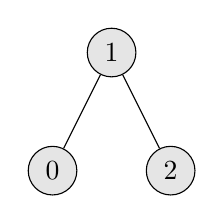
\begin{tikzpicture}
[every node/.style={draw, circle, fill=gray!20!, minimum size=5mm}]
\node{1}
child{node{0}}
child{node{2}};
\end{tikzpicture}
\end{figure}
 
\textbf{Output}: 

\begin{figure}[H]
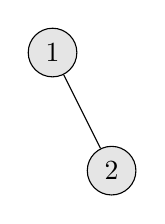
\begin{tikzpicture}
[every node/.style={draw, circle, fill=gray!20!, minimum size=5mm}]
\node{1}
child[missing]
child{node{2}};
\end{tikzpicture}
\end{figure}

\end{flushleft}

\paragraph{Example 2:}
\begin{flushleft}


\textbf{Input}:  $L = 1$,  $R = 3$
 
%    3
%   / \
%  0   4
%   \
%    2
%   /
%  1



\begin{figure}[H]
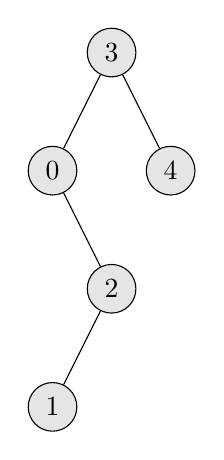
\begin{tikzpicture}
[every node/.style={draw, circle, fill=gray!20!, minimum size=5mm}]
\node{3}
child{node{0} child[missing] child{node{2} child{node{1}} child[missing] } }
child{node{4}};
\end{tikzpicture}
\end{figure}

\textbf{Output}:

\begin{figure}[H]
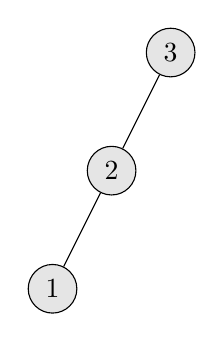
\begin{tikzpicture}
[every node/.style={draw, circle, fill=gray!20!, minimum size=5mm}]
\node{3}
child{node{2} child{node{1}} child[missing]}
child[missing];
\end{tikzpicture}
\end{figure} 
\end{flushleft}

\subsection{Recursion}
Since the given binary tree is a binary search tree, we know that 

\begin{itemize}
\item If root node's value $x$ is less than $L$, we will trim the right child tree.
\item If root node's value $x$ is larger than $R$, we will trim the left child tree.
\item If root node's value $x$ is in the range $[L, R]$, trim the left child tree for range $[L, x]$ and trim the right child tree for range $[x, R]$. The returned nodes will be the root's new left and right child.
\end{itemize}
% \section{670 --- Maximum Swap}
Given a non-negative integer, $x$, you could swap two digits at most once to get the maximum valued number. Return the maximum valued number you could get.

\paragraph{Example 1:}

\begin{flushleft}
\textbf{Input}: 2736

\textbf{Output}: 7236

\textbf{Explanation}: Swap the number 2 and the number 7.

\end{flushleft}

\paragraph{Example 2:}

\begin{flushleft}
\textbf{Input}: 9973

\textbf{Output}: 9973

\textbf{Explanation}: No swap.
\end{flushleft}

\paragraph{Note:}

\begin{itemize}
\item  The given number is in the range $[0, 10^8]$
\end{itemize}

\subsection{Maximum/Minimum Prefix}
\begin{itemize}
\item 因为最多只能交换一次,所以必须找到从左向右的最小值和从右向左的最大值在从左至右的第一个交会点。这样交换才能使获得的数字最大化。
\item 比如数字$2736$,从左向右的最小值分别为$2,2,2,2$,而从右向左的最大值分别为$7,7,6,6$,可见在第一个位置两个值就不相同了,所以交换该位置的最小值和最大值得到的数为$7236$。
\item 又比如数字$9973$,从左向右的最小值分别为$9,9,7,3$,而从右向左的最大值分别为$9,9,7,3$。没有一个位置处,这两个值是不相同的,所以无法交换,最大的数仍然为其本身。
\item 在实现的时候,不仅需要知道最小值和最大值的大小,还需要知道其位置,所以数组的每个元素存放的是最小和最大值在数组中的位置。
\end{itemize}
% \section{671 --- Second Minimum Node In a Binary Tree}
Given a non-empty special binary tree consisting of nodes with the non-negative value, where each node in this tree has exactly \textbf{two} or \textbf{zero} sub-node. If the node has \textbf{two} sub-nodes, then this node's value is the smaller value among its two sub-nodes. 

More formally, the property \lstinline[language=Java, basicstyle=\small\ttfamily, keywordstyle=\bfseries\color{green!40!black}]|root.val = min(root.left.val, root.right.val)| always holds.

Given such a binary tree, you need to output the second minimum value in the set made of all the nodes' value in the whole tree.

If no such second minimum value exists, output $-1$ instead.

\paragraph{Example 1:}

\begin{flushleft}

\textbf{Input}:
\begin{figure}[H]
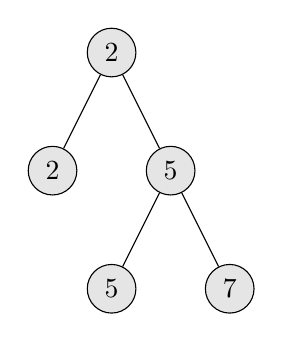
\begin{tikzpicture}
[every node/.style={draw, circle, fill=gray!20!, minimum size=5mm}]
\node{2}
child{node{2}}
child{node{5} child{node{5}} child{node{7}} };
\end{tikzpicture}
\end{figure} 

\textbf{Output}: 5

\textbf{Explanation}: The smallest value is 2, the second smallest value is 5.

\end{flushleft} 

\paragraph{Example 2:}

\begin{flushleft}

\textbf{Input}: 

\begin{figure}[H]
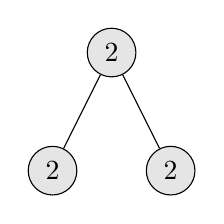
\begin{tikzpicture}
[every node/.style={draw, circle, fill=gray!20!, minimum size=5mm}]
\node{2}
child{node{2}}
child{node{2}};
\end{tikzpicture}
\end{figure}

\textbf{Output}: $-1$

\textbf{Explanation}: The smallest value is 2, but there isn't any second smallest value.
\end{flushleft}

\subsection{Depth First Search}
The problem asks for the 2nd minimum value, thus we may need to track both minimum, say, $x$, and 2nd minimum value, say $y$, at same time. From the property of the tree, we can easily know that the value of the root node is the minimum value of entire tree. Thus, $x$ will be the value of the root node.

When traversing the tree to a node, say $t$, if \lstinline[language=Java, basicstyle=\small\ttfamily, keywordstyle=\bfseries\color{green!40!black}]|t.val > x|, we know all values in the subtree root at $t$ are at least \lstinline[language=Java, basicstyle=\small\ttfamily, keywordstyle=\bfseries\color{green!40!black}]|t.val|, so there cannot be a better candidate for the second minimum in this subtree than \lstinline[language=Java, basicstyle=\small\ttfamily, keywordstyle=\bfseries\color{green!40!black}]|t.val|. Hence, we do not need to search this subtree.

Also, as we only care about the second minimum $y$, we do not need to record any values that are larger than our current candidate for the 2nd minimum value.

\setcounter{lstlisting}{0}
\begin{lstlisting}[style=customc, caption={DFS}]
int findSecondMinimumValue( TreeNode* root )
{
    int ans = -1;

    //root->val is the global minimum value
    //of entire tree
    dfs( root, root->val, ans );

    //since the tree only contains
    //non-negative number
    //if ans < 0, 2nd minimum has not been found
    return ans < 0 ? -1 : ans;
}

void dfs( TreeNode* node, int min_v, int& y )
{
    if( node )
    {
        if( node->val > min_v )
        {
            if( ( y < 0 ) || ( y > node->val ) )
            {
                //y < 0 means this is the
                //firt time to set y,
                //i.e. 2nd minimum value
                y = node->val;
            }
        }
        else if( node->val == min_v )
        {
            //recursively go to
            //left and right subtree
            dfs( node->left, min_v, y );
            dfs( node->right, min_v, y );
        }
    }
}
\end{lstlisting}
% \section{672 --- Bulb Switcher II}
There is a room with $n$ lights which are turned on initially and 4 buttons on the wall. After performing exactly $m$ unknown operations towards buttons, you need to return how many different kinds of status of the $n$ lights could be.

Suppose $n$ lights are labeled as number $[1, 2, 3, \ldots, n]$, function of these 4 buttons are given below:

\begin{enumerate}
\item Flip all the lights.
\item Flip lights with even numbers.
\item Flip lights with odd numbers.
\item Flip lights with $(3k + 1)$ numbers, $k = 0, 1, 2, \ldots$

\end{enumerate}
 

\paragraph{Example 1:}
\begin{flushleft}

\textbf{Input}: $n = 1$, $m = 1$.

\textbf{Output}: 2

\textbf{Explanation}: Status can be: \lstinline[language=Java, basicstyle=\small\ttfamily, keywordstyle=\bfseries\color{green!40!black}]|[on], [off]|
\end{flushleft}
 

\paragraph{Example 2:}
\begin{flushleft}

\textbf{Input}: $n = 2$, $m = 1$.

\textbf{Output}: 3

\textbf{Explanation}: Status can be: \lstinline[language=Java, basicstyle=\small\ttfamily, keywordstyle=\bfseries\color{green!40!black}]|[on, off], [off, on], [off, off]|
\end{flushleft}
 

\paragraph{Example 3:}

\begin{flushleft}


\textbf{Input}: $n = 3$, $m = 1$.

\textbf{Output}: 4

\textbf{Explanation}: 

Status can be: \lstinline[language=Java, basicstyle=\small\ttfamily, keywordstyle=\bfseries\color{green!40!black}]|[off, on, off], [on, off, on], [off, off, off], [off, on, on]|.
\end{flushleft}

\paragraph{Note:} 
\begin{itemize}
\item $n$ and $m$ both fit in range \lstinline[language=Java, basicstyle=\small\ttfamily, keywordstyle=\bfseries\color{green!40!black}]|[0, 1000]|.
\end{itemize}

\subsection{Reduce Search Space}
Give the conditions, we know the search space is very large: there will be $2^N$ states of lights and $4^M$ operation sequences. Reducing the search space must be done first.

Actually, the first 6 lights uniquely determine the rest of the lights. This is because every operation that modifies the $x$-th light also changes the $(x+6)$-th light.

Regarding to operations: 

\begin{itemize}
\item operations are commutative: doing operation $A$ followed by $B$ is the same as doing operation $B$ followed by $A$. So we can assume we do all the operations in order. 
\item Doing the same operation twice in a row is the same as doing nothing. Hence, we can mark the operation state as 1 when it is running odd times and 0 for even times. For example, if current operation state is $9$ (\lstinline[language=C++, basicstyle=\small\ttfamily, keywordstyle=\bfseries\color{green!40!black}]|0b1001|), the operation 1 and 4 will perform odd times.

For the four operations, we will have total $2^4=16$ operation states by treating each operation as a bit position in a integer. Thus if $m > 4$, the results will repeat the results from $m \leq 4$. 
\end{itemize}

Now, given $m$, we will try all 16 operation states to see if a state is possible to make $m$ operations. In each state, we firstly check how many operations will be taken by odd times, say the result is $x$.
\begin{itemize}
\item If $x > m$, we will skip this state.
\item If $x \leq m$, this state is possible only if $\bmod(x, 2)=\bmod(m,2)$. The reason is that: in this case, we need to perform $x$ operations odd times. If $x$ is odd number, the total number of operations would be odd. Conversely, if $x$ is even number, total number of operations must be even.  


\item For each possible state, since the first 6 lights uniquely determine the rest of the digits, we can make use of 6-bits in a integer to record the states of the bulbs. Put these states into a hash set. Finally, the number of elements in this hash set will be the answer
\end{itemize}

\setcounter{lstlisting}{0}
\begin{lstlisting}[style=customc, caption={Reduce Search Space}]
int flipLights( int n, int m )
{
    n = ( min )( n, 6 );

    auto get_ones = []( int n )
    {
        int ones = 0;
        while( n )
        {
            ++ones;
            n = n & ( n - 1 );
        }

        return ones;
    };

    //n may be less than 6
    //in this case, we don't need
    //6 bits, we only n bits
    int shift = ( max )( 0, 6 - n );

    int parity = ( m & 1 );

    unordered_set<int> l_states;

    for( int state = 0; state < 16; ++state )
    {
        int odd_opers = get_ones( state );

        //the number of odd operations should less than m
        //and the odd/even should is same as m
        if( ( odd_opers <= m ) && ( ( odd_opers & 1 ) == parity ) )
        {
            int mask = 1;

            int lights = 0;

            if( mask & state )
            {
                //do operation 1: 111111
                lights ^= ( 63 >> shift );
            }

            mask <<= 1;

            if( mask & state )
            {
                //do operation 2: 010101
                lights ^= ( 21 >> shift );
            }

            mask <<= 1;

            if( mask & state )
            {
                //do operation 3: 101010
                lights ^= ( 42 >> shift );
            }

            mask <<= 1;

            if( mask & state )
            {
                //do operation 4: 100100
                lights ^= ( 36 >> shift );
            }

            l_states.insert( lights );
        }

    }

    return static_cast< int >( l_states.size() );
}
\end{lstlisting}



% \section{673 --- Number of Longest Increasing Subsequence}
Given an unsorted array of integers, $A$,  find the number of longest increasing subsequence.

\paragraph{Example 1:}
\begin{flushleft}


\textbf{Input}: \lstinline[language=C++, basicstyle=\small\ttfamily, keywordstyle=\bfseries\color{green!40!black}]|[1,3,5,4,7]|

\textbf{Output}: 2

\textbf{Explanation}: The two longest increasing subsequence are \lstinline[language=C++, basicstyle=\small\ttfamily, keywordstyle=\bfseries\color{green!40!black}]|[1, 3, 4, 7]| and \lstinline[language=C++, basicstyle=\small\ttfamily, keywordstyle=\bfseries\color{green!40!black}]|[1, 3, 5, 7]|.
\end{flushleft}

\paragraph{Example 2:}
\begin{flushleft}


\textbf{Input}: \lstinline[language=C++, basicstyle=\small\ttfamily, keywordstyle=\bfseries\color{green!40!black}]|[2,2,2,2,2]|

\textbf{Output}: 5

\textbf{Explanation}: 

The length of longest continuous increasing subsequence is 1, and there are 5 subsequences' length is 1, so output 5.
\end{flushleft}

\paragraph{Note:} 
\begin{itemize}
\item Length of the given array will be not exceed 2000 and the answer is guaranteed to be fit in 32-bit \lstinline[language=C++, basicstyle=\small\ttfamily, keywordstyle=\bfseries\color{green!40!black}]|signed int|.
\end{itemize}

\subsection{Segment Tree}
Many problems require that we give results based on query over a range or segment of available data. This can be a tedious and slow process, especially if the number of queries is large and repetitive. A segment tree let's us process such queries efficiently in logarithmic order of time.

Segment Trees have applications in areas of computational geometry and geographic information systems. For example, we may have a large number of points in space at certain distances from a central reference/origin point. Suppose we have to lookup the points which are in a certain range of distances from our origin. An ordinary lookup table would require a linear scan over all the possible points or all possible distances (think hash-maps). Segment Trees lets us achieve this in logarithmic time with much less space cost. Such a problem is called Planar Range Searching. Solving such problems efficiently is critical, especially when dealing with dynamic data which changes fast and unpredictably (for example, a radar system for air traffic.)

A segment tree is a binary tree where each node represents an interval. Generally a node would store one or more properties of an interval which can be queried later.

A typical example of using segment tree is \textbf{Range Sum Query}. Suppose we are given an array $A$ with size $n$

\begin{enumerate}
\item The root of the segment tree typically represents the entire interval of data. This would be $A[0:n-1]$.
\item Each leaf of the tree represents a range comprising of just a single element. Thus the leaves represent $A[0]$, $A[1]$ and so on until $A[n-1]$.
\item The internal nodes of the tree would represent the \textbf{merged} or \textbf{union} result of their children nodes.
\item Each of the children nodes could represent approximately half of the range represented by their parent.
\end{enumerate}

A segment tree for an $n$ element range can be represented using an array of size $\approx 4\times n$. This ensures that the built segment tree as a complete binary tree, which in turn ensures that the height of the tree is upper-bounded by the logarithm of the size of our input.

The segment tree algorithm include three methods: \textbf{build}, \textbf{query} and \textbf{update}.

\begin{enumerate}
\item \textbf{build}: Build the tree from the original data
\setcounter{lstlisting}{0}
\begin{lstlisting}[style=customc, caption={Build}]
// call this method as build(arr, 0, 0, n-1);
// Here A[] is input array and n is its size.

void buildSegTree( vector<int>& A, int treeIndex, int lo, int hi )
{
    if( lo == hi )
    {
        // leaf node. store value in node.
        tree[treeIndex] = A[lo];
        return;
    }

    int mid = lo + ( hi - lo ) / 2; // recurse deeper for children.

    //build left tree
    buildSegTree( A, 2 * treeIndex + 1, lo, mid );

    //build right tree
    buildSegTree( A, 2 * treeIndex + 2, mid + 1, hi );

    // merge build results
    tree[treeIndex] = merge( tree[2 * treeIndex + 1], tree[2 * treeIndex + 2] );
}
\end{lstlisting}
The method builds the entire tree in a bottom up fashion. When the condition \lstinline[language=C++, basicstyle=\small\ttfamily, keywordstyle=\bfseries\color{green!40!black}]|lo = hi| is satisfied, we are left with a range comprising of just a single element (which happens to be \lstinline[language=C++, basicstyle=\small\ttfamily, keywordstyle=\bfseries\color{green!40!black}]|A[lo]|). This constitutes a leaf of the tree. The rest of the nodes are built by merging the results of their two children. \lstinline[language=C++, basicstyle=\small\ttfamily, keywordstyle=\bfseries\color{green!40!black}]|treeIndex| is the index of the current node of the segment tree which is being processed.
\item \textbf{query}: Read/Query on an interval or segment of the data.

\begin{lstlisting}[style=customc, caption={Query/Read}]
// call this method as query(tree, 0, 0, n-1, i, j);
// Here [i,j] is the range/interval we are querying.
// This method relies on "null" nodes being equivalent to storing zero.
int query( vector<int>& tree, int treeIndex, int lo, int hi, int i, int j )
{
    // query for arr[i..j]

    if( lo > j || hi < i )
    {
        // segment completely outside range
        return 0; // represents a null node
    }

    if( i <= lo && j >= hi )
    {
        // segment completely inside range
        return tree[treeIndex];
    }

    // partial overlap of current segment and queried range.
    // Recurse deeper.
    int mid = lo + ( hi - lo ) / 2;

    if( i > mid )
    {
        return query( tree, 2 * treeIndex + 2, mid + 1, hi, i, j );
    }
    else if( j <= mid )
    {
        return query( tree, 2 * treeIndex + 1, lo, mid, i, j );
    }

    int leftQuery = query( tree, 2 * treeIndex + 1, lo, mid, i, mid );

    int rightQuery = query( tree, 2 * treeIndex + 2, mid + 1, hi, mid + 1, j );

    // merge query results
    return merge( leftQuery, rightQuery );
}
\end{lstlisting}
The method returns a result when the queried range matches exactly with the range represented by a current node. Else it digs deeper into the tree to find nodes which match a portion of the node exactly.

\item \textbf{update}: Update the value of an element.

\begin{lstlisting}[style=customc, caption={Update}]
// call this method as update(tree, 0, 0, n-1, i, val);
// Here you want to update the value at index i with value val.
void update( vector<int>& tree, int treeIndex, int lo, int hi, int arrIndex, int val )
{
    if( lo == hi )
    {
        // leaf node. update element.
        tree[treeIndex] = val;
        return;
    }

    // recurse deeper for appropriate child
    int mid = lo + ( hi - lo ) / 2;

    if( arrIndex > mid )
    {
        update( tree, 2 * treeIndex + 2, mid + 1, hi, arrIndex, val );
    }
    else if( arrIndex <= mid )
    {
        update( 2 * treeIndex + 1, lo, mid, arrIndex, val );
    }

    // merge updates
    tree[treeIndex] = merge( tree[2 * treeIndex + 1], tree[2 * treeIndex + 2] );
}
\end{lstlisting}
This is similar to \textbf{build}. We update the value of the leaf node of our tree which corresponds to the updated element. Later the changes are propagated through the upper levels of the tree straight to the root.
\end{enumerate}

\subsubsection{Lazy Propagation}
What we have been discussing is updating single elements only. That happens in logarithmic time and it's pretty efficient.

But what if we had to update a range of elements? By current method, each element would have to be updated independently. This will incur some run time cost.

The construction of a tree poses another issue called \textbf{ancestral locality}. Ancestors of adjacent leaves are guaranteed to be common at some levels of the tree. Updating each of these leaves individually would mean that we process their common ancestors multiple times. 

Another problem is that queried ranges do not contain frequently updated elements. We might be wasting time updating nodes which are rarely going to be accessed/read.

Using \textbf{Lazy Propagation} allows us to overcome all of these problems by reducing wasteful computations and processing nodes on-demand.

As the name suggests, we update nodes lazily. In short, we try to postpone updating descendants of a node, until the descendants themselves need to be accessed.

For the purpose of applying it to the \textbf{Range Sum Query} problem, we assume that the \textbf{update} operation on a range, increments each element in the range by some amount $x$.

We use another array \lstinline[language=C++, basicstyle=\small\ttfamily, keywordstyle=\bfseries\color{green!40!black}]|lazy[]| which is the same size as our segment tree array \lstinline[language=C++, basicstyle=\small\ttfamily, keywordstyle=\bfseries\color{green!40!black}]|tree[]| to represent a lazy node. \lstinline[language=C++, basicstyle=\small\ttfamily, keywordstyle=\bfseries\color{green!40!black}]|lazy[i]| holds the amount by which the node \lstinline[language=C++, basicstyle=\small\ttfamily, keywordstyle=\bfseries\color{green!40!black}]|tree[i]| needs to be incremented, when that node is finally accessed or queried. When \lstinline[language=C++, basicstyle=\small\ttfamily, keywordstyle=\bfseries\color{green!40!black}]|lazy[i]| is zero, it means that node \lstinline[language=C++, basicstyle=\small\ttfamily, keywordstyle=\bfseries\color{green!40!black}]|tree[i]| is not lazy and has no pending updates.

\paragraph{Updating a range lazily}

This is a three step process:

\begin{enumerate}
\item Normalize the current node. This is done by removing laziness. We simply increment the current node by appropriate amount to remove it's laziness. Then we mark its children to be lazy as the descendants haven't been processed yet.
\item Apply the current update operation to the current node if the current segment lies inside the update range.
\item Recurse for the children as you would normally to find appropriate segments to update.
\end{enumerate}

\begin{lstlisting}[style=customc, caption={Update Lazily}]
//call this method as updateLazily(0,0,n-1,range_start,range_end, val);
//here we want to update the range [range_start, range_end] with value (val)
void updateLazily( int treeIndex, int lo, int hi, int range_start, int range_end, int val )
{
    if( lazy[treeIndex] != 0 )
    {
        //this node is lazy
        //normalize current node by removing laziness
        tree[treeIndex] += ( hi - lo + 1 ) * lazy[treeIndex];

        if( lo != hi )
        {
            //update lazy[] for children
            lazy[2 * treeIndex + 1] += lazy[treeIndex];
            lazy[2 * treeIndex + 2] += lazy[treeIndex];
        }

        //current node is processed
        //no longer lazy
        lazy[treeIndex] = 0;
    }

    if( ( lo > hi ) || ( lo > range_end ) || ( hi < range_start ) )
    {
        //out of range
        return;
    }

    if( ( range_start <= lo ) && ( hi <= range_end ) )
    {
        //segement is fully within the update range
        //update segment
        tree[treeIndex] += ( hi - lo + 1 ) * val;

        if( lo != hi )
        {
            //update lazy[] for children
            lazy[2 * treeIndex + 1] += val;
            lazy[2 * treeIndex + 2] += val;
        }

        return;
    }

    int mid = lo + ( hi - lo ) / 2;

    //recurse deeper for appropriate child
    updateLazily( 2 * treeIndex + 1, lo, mid, range_start, range_end, val );
    updateLazily( 2 * treeIndex + 1, mid + 1, hi, range_start, range_end, val );

    //merge updates
    tree[treeIndex] = tree[2 * treeIndex + 1] + tree[2 * treeIndex + 2];
}
\end{lstlisting}

\paragraph{Querying a lazily propagated tree}

This is a two step process:
\begin{enumerate}
\item Normalize the current node by removing laziness. This step is the same as the \textbf{update} step.
\item Recursively deep into the children to find appropriate segments which fit in queried range.
\end{enumerate}

\begin{lstlisting}[style=customc, caption={Query Lazily}]
// call this method as queryLazily(0, 0, n-1, range_start, range_end);
// Here [range_start, range_end] is the range/interval we are querying.
// This method relies on "null" nodes being equivalent to storing zero.
int queryLazily( int treeIndex, int lo, int hi, int range_start, int range_end )
{
    //query for original array A[range_start, range_end]
    if( ( lo > range_end ) || ( hi < range_start ) )
    {
        //segment is completely outside range
        //return a value represent null node
        return 0;
    }

    if( lazy[treeIndex] )
    {
        //this node is lazy
        //normalize current node by removing laziness
        tree[treeIndex] += ( hi - lo + 1 ) * lazy[treeIndex];

        if( lo != hi )
        {
            //update lazy[] for children nodes
            lazy[2 * treeIndex + 1] += lazy[treeIndex];
            lazy[2 * treeIndex + 2] += lazy[treeIndex];
        }

        //current node is processed
        //it is no longer lazy
        lazy[treeIndex] = 0;
    }

    if( ( range_start <= lo ) && ( hi <= range_end ) )
    {
        //segment is completely inside the query range
        //return the node
        return tree[treeIndex];
    }

    //otherwise, segement is overlap with query range
    int mid = ( hi + lo ) / 2;

    if( range_start > mid )
    {
        return queryLazily( treeIndex * 2 + 1, mid + 1, hi, range_start, range_end );
    }
    else if( range_end <= md )
    {
        return queryLazily( treeIndex * 2 + 2, lo, mid, range_start, range_end );
    }

    int leftQuery = queryLazily( 2 * treeIndex + 1, lo, mid, range_start, mid );
    int rightQuery = queryLazily( 2 * treeIndex + 2, mid + 1, hi, mid + 1, range_end );

    //merge query results
    return leftQuery + rightQuery;
}
\end{lstlisting}

\paragraph{Note:} The following lines:

\begin{lstlisting}[style=customc, caption={Notes}]
// normalize current node by removing laziness
tree[treeIndex] += ( hi - lo + 1 ) * lazy[treeIndex];

// update segment
tree[treeIndex] += ( hi - lo + 1 ) * val;

// merge updates
tree[treeIndex] = tree[2 * treeIndex + 1] + tree[2 * treeIndex + 2];
\end{lstlisting}

are specific to the \textbf{Range Sum Query} problem. Different problems may have their own updating and merging schemes.
% \section{674 --- Longest Continuous Increasing Subsequence}
Given an unsorted array of integers, $A$, find the length of longest continuous increasing subsequence (subarray).

\paragraph{Example 1:}
\begin{flushleft}


\textbf{Input}: \lstinline[language=Java, basicstyle=\small\ttfamily, keywordstyle=\bfseries\color{green!40!black}]|[1,3,5,4,7]|

\textbf{Output}: 3

\textbf{Explanation}: 

The longest continuous increasing subsequence is \lstinline[language=Java, basicstyle=\small\ttfamily, keywordstyle=\bfseries\color{green!40!black}]|[1,3,5]|, its length is 3.
 
Even though \lstinline[language=Java, basicstyle=\small\ttfamily, keywordstyle=\bfseries\color{green!40!black}]|[1,3,5,7]| is also an increasing subsequence, it's not a continuous one where 5 and 7 are separated by 4. 
\end{flushleft}

\paragraph{Example 2:}

\begin{flushleft}
\textbf{Input}: \lstinline[language=Java, basicstyle=\small\ttfamily, keywordstyle=\bfseries\color{green!40!black}]|[2,2,2,2,2]|

\textbf{Output}: 1

Explanation: The longest continuous increasing subsequence is \lstinline[language=Java, basicstyle=\small\ttfamily, keywordstyle=\bfseries\color{green!40!black}]|[2]|, its length is 1. 
\end{flushleft}

\subsection{Sliding Window}
This question is asking for continuous sub-sequence. We maintain $x$ to record current increasing continuous sub-sequence length. When the sub-sequence is broken, update the global maximum length by $x$ and then reset $x$ to 1. 

\setcounter{lstlisting}{0}
\begin{lstlisting}[style=customc, caption={Sliding Window}]
int findLengthOfLCIS( vector<int>& nums )
{
    if( nums.empty() )
    {
        return 0;
    }

    //current length of increasing continuous subsequence
    int len = 1;

    //global maximum length
    int best = 1;

    for( size_t i = 1; i < nums.size(); ++i )
    {
        if( nums[i] > nums[i - 1] )
        {
            ++len;
        }
        else
        {
            //current continuous subsequence is broken
            //update global maximum length and
            //reset length to 1
            best = ( max )( len, best );
            len = 1;
        }
    }

    //To update for the subsequence ending with last element
    best = ( max )( len, best );

    return best;
}
q
\end{lstlisting}

% \section{675 --- Cut Off Trees for Golf Event}
You are asked to cut off trees in a forest for a golf event. The forest is represented as a non-negative 2D map, in this map:

\begin{itemize}
\item 0 represents the \textbf{obstacle} can't be reached.
\item 1 represents the \textbf{ground} can be walked through.
\item \textbf{The place with number bigger than 1} represents a \textbf{tree} can be walked through, and this positive number represents the tree's height.
\end{itemize}
 

You are asked to cut off all the trees in this forest in the order of tree's height - always cut off the tree with lowest height first. And after cutting, the original place has the tree will become a grass (value 1).

You will start from the point (0, 0) and you should output the minimum steps you need to walk to cut off all the trees. If you can't cut off all the trees, output $-1$ in that situation.

You are guaranteed that no two trees have the same height and there is at least one tree needs to be cut off.

\paragraph{Example 1:}

\begin{flushleft}
\textbf{Input}:
\[
\begin{bmatrix}
1 & 2 & 3\\
0 & 0 & 4\\
7 & 6 & 5
\end{bmatrix}
\] 

\textbf{Output}: 6

\end{flushleft}
 

\paragraph{Example 2:}
\begin{flushleft}

\textbf{Input}: 

\[
\begin{bmatrix}
1 & 2 & 3\\
0 & 0 & 0\\
7 & 6 & 5
\end{bmatrix}
\] 

\textbf{Output}: $-1$
 

\end{flushleft}

\paragraph{Example 3:}
\begin{flushleft}


\textbf{Input}: 
\[
\begin{bmatrix}
2 & 3 & 4\\
0 & 0 & 5\\
8 & 7 & 6
\end{bmatrix}
\]

\textbf{Output}: 6

\textbf{Explanation}: 

You started from the point \lstinline[language=Java, basicstyle=\small\ttfamily, keywordstyle=\bfseries\color{green!40!black}]|(0,0)| and you can cut off the tree in \lstinline[language=Java, basicstyle=\small\ttfamily, keywordstyle=\bfseries\color{green!40!black}]|(0,0)| directly without walking.
\end{flushleft}

\subsection{Finding Shortest Path}

% \section{676 --- Implement Magic Dictionary}
Implement a magic directory with \lstinline[language=Java, basicstyle=\small\ttfamily, keywordstyle=\bfseries\color{green!40!black}]|buildDict|, and \lstinline[language=Java, basicstyle=\small\ttfamily, keywordstyle=\bfseries\color{green!40!black}]|search| methods.

For the method \lstinline[language=Java, basicstyle=\small\ttfamily, keywordstyle=\bfseries\color{green!40!black}]|buildDict|, you'll be given a list of non-repetitive words to build a dictionary.

For the method search, you'll be given a word, and judge whether if you modify exactly one \textbf{character} into another \textbf{character} in this word, the modified word is in the dictionary you just built.

\paragraph{Example 1:}
\begin{flushleft}


\textbf{Input}: \lstinline[language=Java, basicstyle=\small\ttfamily, keywordstyle=\bfseries\color{green!40!black}]|buildDict(["hello", "leetcode"])|, \textbf{Output}: \lstinline[language=Java, basicstyle=\small\ttfamily, keywordstyle=\bfseries\color{green!40!black}]|Null|

\textbf{Input}: \lstinline[language=Java, basicstyle=\small\ttfamily, keywordstyle=\bfseries\color{green!40!black}]|search("hello")|, \textbf{Output}: \lstinline[language=Java, basicstyle=\small\ttfamily, keywordstyle=\bfseries\color{green!40!black}]|False|

\textbf{Input}: \lstinline[language=Java, basicstyle=\small\ttfamily, keywordstyle=\bfseries\color{green!40!black}]|search("hhllo")|, \textbf{Output}: \lstinline[language=Java, basicstyle=\small\ttfamily, keywordstyle=\bfseries\color{green!40!black}]|True|

\textbf{Input}: \lstinline[language=Java, basicstyle=\small\ttfamily, keywordstyle=\bfseries\color{green!40!black}]|search("hell")|, \textbf{Output}: \lstinline[language=Java, basicstyle=\small\ttfamily, keywordstyle=\bfseries\color{green!40!black}]|False|

\textbf{Input}: \lstinline[language=Java, basicstyle=\small\ttfamily, keywordstyle=\bfseries\color{green!40!black}]|search("leetcoded")|, \textbf{Output}: \lstinline[language=Java, basicstyle=\small\ttfamily, keywordstyle=\bfseries\color{green!40!black}]|False|
\end{flushleft}
\paragraph{Note:}

\begin{itemize}
\item  You may assume that all the inputs are consist of lowercase letters \texttt{a} -- \texttt{z}.
\end{itemize}

\subsection{Hash Set}
If the word can be found by changing only one letter, this word must have the same size as the one in the dictionary. Thus we can group all the input strings per their lengths.

During the search, we iterate over the input word. Try all lowercase letters except the one in current position and see if we can find the result string in the strings that has same size as the input word.

\setcounter{lstlisting}{0}
\begin{lstlisting}[style=customc, caption={Hash}]
class MagicDictionary
{
public:
    /** Initialize your data structure here. */
    MagicDictionary()
    {
    }

    /** Build a dictionary through a list of words */
    void buildDict( vector<string> dict )
    {
        swap( m_words, dict );

        //group the words
        //per their size
        for( const auto& word : m_words )
        {
            auto key = word.size();

            auto it = m_dict.find( key );

            string_view sv( word.c_str(), word.size() );

            if( it == m_dict.end() )
            {

                m_dict.emplace( key, unordered_set<string_view> {sv} );
            }
            else
            {
                it->second.insert( sv );
            }
        }

    }

    /** Returns if there is any word in the trie that equals to the given word after modifying exactly one character */
    bool search( string word )
    {

        auto it = m_dict.find( word.size() );

        if( it == m_dict.end() )
        {
            return false;
        }

        //find in the strings with same size as word
        for( size_t i = 0; i < word.size(); ++i )
        {
            char wc = word[i];

            for( char c = 'a'; c <= 'z'; ++c )
            {
                if( c == wc )
                {
                    continue;
                }

                //change word by modifying current letter
                word[i] = c;

                string_view sv( word.c_str(), word.size() );

                if( it->second.find( sv ) != it->second.end() )
                {
                    //found target
                    return true;
                }
            }

            //restore word
            word[i] = wc;
        }

        return false;
    }

    //the dictionry used in the algorithm
    unordered_map<size_t, unordered_set<string_view>> m_dict;

    //store the input dictionary
    vector<string> m_words;


};

/**
 * Your MagicDictionary object will be instantiated and called as such:
 * MagicDictionary* obj = new MagicDictionary();
 * obj->buildDict(dict);
 * bool param_2 = obj->search(word);
 */
\end{lstlisting}
% \section{677 --- Map Sum Pairs}
Implement a \lstinline[language=Java, basicstyle=\small\ttfamily, keywordstyle=\bfseries\color{green!40!black}]|MapSum| class with \lstinline[language=Java, basicstyle=\small\ttfamily, keywordstyle=\bfseries\color{green!40!black}]|insert|, and \lstinline[language=Java, basicstyle=\small\ttfamily, keywordstyle=\bfseries\color{green!40!black}]|sum| methods.

For the method \lstinline[language=Java, basicstyle=\small\ttfamily, keywordstyle=\bfseries\color{green!40!black}]|insert|, you'll be given a pair of \lstinline[language=Java, basicstyle=\small\ttfamily, keywordstyle=\bfseries\color{green!40!black}]|(string, integer)|. The \lstinline[language=Java, basicstyle=\small\ttfamily, keywordstyle=\bfseries\color{green!40!black}]|string| represents the key and the \lstinline[language=Java, basicstyle=\small\ttfamily, keywordstyle=\bfseries\color{green!40!black}]|integer| represents the value. If the key already existed, then the original key-value pair will be overridden to the new one.

For the method \lstinline[language=Java, basicstyle=\small\ttfamily, keywordstyle=\bfseries\color{green!40!black}]|sum|, you'll be given a string representing the prefix, and you need to return the sum of all the pairs' value whose key starts with the prefix.

\paragraph{Example 1:}

\begin{flushleft}


\textbf{Input}: \lstinline[language=Java, basicstyle=\small\ttfamily, keywordstyle=\bfseries\color{green!40!black}]|insert("apple", 3)|, \textbf{Output}: \lstinline[language=Java, basicstyle=\small\ttfamily, keywordstyle=\bfseries\color{green!40!black}]|Null|

\textbf{Input}: \lstinline[language=Java, basicstyle=\small\ttfamily, keywordstyle=\bfseries\color{green!40!black}]|sum("ap")|, \textbf{Output}: 3

\textbf{Input}: \lstinline[language=Java, basicstyle=\small\ttfamily, keywordstyle=\bfseries\color{green!40!black}]|insert("app", 2)|, Output: \lstinline[language=Java, basicstyle=\small\ttfamily, keywordstyle=\bfseries\color{green!40!black}]|Null|

\textbf{Input}: \lstinline[language=Java, basicstyle=\small\ttfamily, keywordstyle=\bfseries\color{green!40!black}]|sum("ap")|, Output: 5

\end{flushleft}

\subsection{Trie}
Since this is for prefix searching, Trie structure is the natural way. For \lstinline[language=Java, basicstyle=\small\ttfamily, keywordstyle=\bfseries\color{green!40!black}]|sum| function, we need a depth first search approach to get the total of all the trie nodes each represents a key.

\setcounter{lstlisting}{0}
\begin{lstlisting}[style=customc, caption={Trie}]
class MapSum
{
public:
    /** Initialize your data structure here. */
    MapSum()
    {
    }

    void insert( string key, int val )
    {
        add( key, val );
    }

    int sum( string prefix )
    {
        int ans = 0;

        auto node = m_root;

        //go to the end node of prefix
        for( const auto c : prefix )
        {
            auto it = node->children.find( c );
            if( it == node->children.end() )
            {
                return 0;
            }

            node = it->second;
        }

        //using dfs to sum all the values
        dfs( node, ans );

        return ans;
    }

private:

    struct Trie
    {
        unordered_map<char, Trie*> children;
        int val = 0;
        unsigned char flag = 0;
    };

    Trie* m_root = new Trie;
    void add( const string& s, int val )
    {
        auto node = m_root;

        for( auto c : s )
        {
            auto it = node->children.find( c );
            if( it == node->children.end() )
            {
                it = node->children.emplace( c, new Trie ).first;
            }
            node = it->second;
        }

        node->flag = 1;
        node->val = val;
    }

    void dfs( Trie* trie, int& total )
    {
        if( !trie )
        {
            return;
        }

        if( trie->flag )
        {
            //add the value
            // of this key to total
            total += trie->val;
        }

        for( const auto& p : trie->children )
        {
            //recursively deeper into the children
            dfs( p.second, total );
        }
    }
};

/**
 * Your MapSum object will be instantiated and called as such:
 * MapSum* obj = new MapSum();
 * obj->insert(key,val);
 * int param_2 = obj->sum(prefix);
 */
\end{lstlisting}
% \section{678 --- Valid Parenthesis String}
Given a string, $s$, containing only three types of characters: \lstinline[language=Java, basicstyle=\small\ttfamily, keywordstyle=\bfseries\color{green!40!black}]|'('|, \lstinline[language=Java, basicstyle=\small\ttfamily, keywordstyle=\bfseries\color{green!40!black}]|')'| and \lstinline[language=Java, basicstyle=\small\ttfamily, keywordstyle=\bfseries\color{green!40!black}]|'*'|, write a function to check whether this string is valid. We define the validity of a string by these rules:

\begin{enumerate}
\item Any left parenthesis \lstinline[language=Java, basicstyle=\small\ttfamily, keywordstyle=\bfseries\color{green!40!black}]|'('| must have a corresponding right parenthesis \lstinline[language=Java, basicstyle=\small\ttfamily, keywordstyle=\bfseries\color{green!40!black}]|')'|.
\item Any right parenthesis \lstinline[language=Java, basicstyle=\small\ttfamily, keywordstyle=\bfseries\color{green!40!black}]|')'| must have a corresponding left parenthesis \lstinline[language=Java, basicstyle=\small\ttfamily, keywordstyle=\bfseries\color{green!40!black}]|'('|.
\item Left parenthesis \lstinline[language=Java, basicstyle=\small\ttfamily, keywordstyle=\bfseries\color{green!40!black}]|'('| must go before the corresponding right parenthesis \lstinline[language=Java, basicstyle=\small\ttfamily, keywordstyle=\bfseries\color{green!40!black}]|')'|.
\item \lstinline[language=Java, basicstyle=\small\ttfamily, keywordstyle=\bfseries\color{green!40!black}]|'*'| could be treated as a single right parenthesis \lstinline[language=Java, basicstyle=\small\ttfamily, keywordstyle=\bfseries\color{green!40!black}]|')'| or a single left parenthesis \lstinline[language=Java, basicstyle=\small\ttfamily, keywordstyle=\bfseries\color{green!40!black}]|'('| or an empty string.
\item An empty string is also valid.
\end{enumerate}

\paragraph{Example 1:}

\begin{flushleft}
\textbf{Input}: \lstinline[language=Java, basicstyle=\small\ttfamily, keywordstyle=\bfseries\color{green!40!black}]|"()"|

\textbf{Output}: \lstinline[language=Java, basicstyle=\small\ttfamily, keywordstyle=\bfseries\color{green!40!black}]|True|

\end{flushleft}

\paragraph{Example 2:}

\begin{flushleft}
\textbf{Input}: \lstinline[language=Java, basicstyle=\small\ttfamily, keywordstyle=\bfseries\color{green!40!black}]|"(*)"|

\textbf{Output}: \lstinline[language=Java, basicstyle=\small\ttfamily, keywordstyle=\bfseries\color{green!40!black}]|True|
\end{flushleft}

\paragraph{Example 3:}

\begin{flushleft}
\textbf{Input}: \lstinline[language=Java, basicstyle=\small\ttfamily, keywordstyle=\bfseries\color{green!40!black}]|"(*))"|

\textbf{Output}: \lstinline[language=Java, basicstyle=\small\ttfamily, keywordstyle=\bfseries\color{green!40!black}]|True|
\end{flushleft}

\paragraph{Note:}

\begin{itemize}
\item The string size will be in the range \lstinline[language=Java, basicstyle=\small\ttfamily, keywordstyle=\bfseries\color{green!40!black}]|[1, 100]|.
\end{itemize}


\subsection{Greedy}
When checking whether the string is valid, we only cared about the number of extra open left parenthesis as parsing through the string. 

For example, when checking whether \lstinline[language=Java, basicstyle=\small\ttfamily, keywordstyle=\bfseries\color{green!40!black}]|'(()())'| is valid, we had a number of extra left parenthesis of \lstinline[language=Java, basicstyle=\small\ttfamily, keywordstyle=\bfseries\color{green!40!black}]|[1, 2, 1, 2, 1, 0]| as we parse through the string: \lstinline[language=Java, basicstyle=\small\ttfamily, keywordstyle=\bfseries\color{green!40!black}]|(| has 1 left bracket, \lstinline[language=Java, basicstyle=\small\ttfamily, keywordstyle=\bfseries\color{green!40!black}]|'(('| has 2, \lstinline[language=Java, basicstyle=\small\ttfamily, keywordstyle=\bfseries\color{green!40!black}]|'(()'| has 1, and so on. This means that after parsing the first $x$ symbols, (which may include asterisks,) we only need to keep track of how many there could have extra left parenthesis.

For example, if we have string \lstinline[language=Java, basicstyle=\small\ttfamily, keywordstyle=\bfseries\color{green!40!black}]|'(***)'|, then as we parse each symbol, the set of possible values for the balance is
\begin{itemize}
\item \lstinline[language=Java, basicstyle=\small\ttfamily, keywordstyle=\bfseries\color{green!40!black}]|[1]| for \lstinline[language=Java, basicstyle=\small\ttfamily, keywordstyle=\bfseries\color{green!40!black}]|'('|;
\item \lstinline[language=Java, basicstyle=\small\ttfamily, keywordstyle=\bfseries\color{green!40!black}]|[0, 1, 2]| for \lstinline[language=Java, basicstyle=\small\ttfamily, keywordstyle=\bfseries\color{green!40!black}]|'(*'|;
\item \lstinline[language=Java, basicstyle=\small\ttfamily, keywordstyle=\bfseries\color{green!40!black}]|[0, 1, 2, 3]| for \lstinline[language=Java, basicstyle=\small\ttfamily, keywordstyle=\bfseries\color{green!40!black}]|'(**'|;
\item \lstinline[language=Java, basicstyle=\small\ttfamily, keywordstyle=\bfseries\color{green!40!black}]|[0, 1, 2, 3, 4]| for \lstinline[language=Java, basicstyle=\small\ttfamily, keywordstyle=\bfseries\color{green!40!black}]|'(***'|, 
\item and \lstinline[language=Java, basicstyle=\small\ttfamily, keywordstyle=\bfseries\color{green!40!black}]|[0, 1, 2, 3]| for \lstinline[language=Java, basicstyle=\small\ttfamily, keywordstyle=\bfseries\color{green!40!black}]|'(***)'|.

\end{itemize}
Furthermore, we can prove these states always form a contiguous interval. Thus, we only need to know the left and right bounds of this interval. That is, we would keep those intermediate states described above as 

\lstinline[language=Java, basicstyle=\small\ttfamily, keywordstyle=\bfseries\color{green!40!black}]|[lo, hi] = [1, 1], [0, 2], [0, 3], [0, 4], [0, 3]|.

\paragraph{Algorithm}

We maintain two varaibles $l$ and $h$ where 

\begin{enumerate}
\item $l$ 表示在有左括号的情况下,将星号当作右括号时左括号的个数(这样做的原因是尽量不多增加右括号的个数)
\item $h$ 表示将星号当作左括号时左括号的个数
\end{enumerate}

When iterating over the string
\begin{itemize}
\item 当遇到左括号时,$l\gets l+1$ and $h\gets h+1$
\item 当遇到右括号时,$l\gets l-1$ only when $l >0$ to make sure $l\geq 0$, and $h\gets h-1$
\item 当遇到星号时,$l\gets l-1$ only when $l >0$ to make sure $l\geq 0$, and $h\gets h+1$ because we treat asterisk as left parenthesis.
\item When $h<0$, 说明就算把星号都当作左括号了,还是不够抵消右括号,直接返回\lstinline[language=C++, basicstyle=\small\ttfamily, keywordstyle=\bfseries\color{green!40!black}]|false|.
\end{itemize}

At the end, we check if $l=0$.

\setcounter{lstlisting}{0}
\begin{lstlisting}[style=customc, caption={Greedy}]
bool checkValidString( string s )
{
    //the number of actual parenthesis
    int l = 0;

    //the number of left parenthesis
    //including asterisks treated as left parenthesis
    int h = 0;

    for( auto c : s )
    {
        if( c == '(' )
        {
            ++l;
            ++h;
        }
        else if( c == ')' )
        {
            //make sure l always
            //no less than 0
            if( l > 0 )
            {
                --l;
            }

            --h;
        }
        else
        {
            if( l > 0 )
            {
                --l;
            }

            //we can treat asterisk
            //as asterisk
            ++h;
        }

        if( h < 0 )
        {
            //too many right parenthesis
            //even if we treat asterisks as
            //left parenthesis
            return false;
        }
    }

    //only valid when
    //actual left parenthesis
    //are complete offset
    //by right parenthesis and
    //asterisk
    return l == 0;
}
\end{lstlisting}

\subsection{Two Stacks}
We can make use of two stacks, $\alpha$ and $\beta$ to track left parenthesis and asterisks. Since the positions are critical, we push each index of left parenthesis and asterisk into corresponding stack.

While iterating 
\begin{enumerate}
\item If it is \lstinline[language=C++, basicstyle=\small\ttfamily, keywordstyle=\bfseries\color{green!40!black}]|')'|, push the index into $\alpha$
\item If it is \lstinline[language=C++, basicstyle=\small\ttfamily, keywordstyle=\bfseries\color{green!40!black}]|'*'|, push the index into $\beta$
\item Otherwise, it is \lstinline[language=C++, basicstyle=\small\ttfamily, keywordstyle=\bfseries\color{green!40!black}]|')'|, we choose to pop from $\alpha$. If $\alpha$ is empty, pop from $\beta$. If both stacks are empty, the expression contains too many \lstinline[language=C++, basicstyle=\small\ttfamily, keywordstyle=\bfseries\color{green!40!black}]|')'|, just return \lstinline[language=C++, basicstyle=\small\ttfamily, keywordstyle=\bfseries\color{green!40!black}]|false|.
\end{enumerate}

After iterations, we may have remaining unmatched \lstinline[language=C++, basicstyle=\small\ttfamily, keywordstyle=\bfseries\color{green!40!black}]|')'|. We need to check if they can be matched by \lstinline[language=C++, basicstyle=\small\ttfamily, keywordstyle=\bfseries\color{green!40!black}]|'*'|. Thus, we iterate $\alpha$ and $\beta$. If we find that a asterisk appears before a left parenthesis, the expression is invalid. 

At the end, check if $\alpha$ is empty. 

\begin{lstlisting}[style=customc, caption={Two Stacks}]
bool checkValidString( string s )
{
    //record index of '('
    stack<size_t> left;
    //record index of '*'
    stack<size_t> ast;

    for( size_t i = 0; i < s.size(); ++i )
    {
        if( s[i] == '(' )
        {
            left.push( i );
        }
        else if( s[i] == '*' )
        {
            ast.push( i );
        }
        else
        {
            if( !left.empty() )
            {
                //match a '('
                left.pop();
            }
            else if( !ast.empty() )
            {
                //match a '*'
                ast.pop();
            }
            else
            {
                //too many ')'
                return false;
            }
        }
    }

    while( !left.empty() && !ast.empty() )
    {
        if( left.top() < ast.top() )
        {
            //match a '(' with '*'
            left.pop();
            ast.pop();
        }
        else
        {
            //'(' cannot be matched
            return false;
        }
    }

    //check if all '(' are matched
    return left.empty();
}
\end{lstlisting}

\subsection{Scan Twice}
We scan the input string $s$ twice

When scan from left to right, we treat \lstinline[language=C++, basicstyle=\small\ttfamily, keywordstyle=\bfseries\color{green!40!black}]|'*'| as \lstinline[language=C++, basicstyle=\small\ttfamily, keywordstyle=\bfseries\color{green!40!black}]|'('|. We make use of a counter $\delta$ to count \lstinline[language=C++, basicstyle=\small\ttfamily, keywordstyle=\bfseries\color{green!40!black}]|'('|. For each \lstinline[language=C++, basicstyle=\small\ttfamily, keywordstyle=\bfseries\color{green!40!black}]|'('| or \lstinline[language=C++, basicstyle=\small\ttfamily, keywordstyle=\bfseries\color{green!40!black}]|'*'|, increments $\delta$. Otherwise, $\delta\gets\delta-1$. Whenever $\delta < 0$, just return \lstinline[language=C++, basicstyle=\small\ttfamily, keywordstyle=\bfseries\color{green!40!black}]|false| because it is showing that there are excess \lstinline[language=C++, basicstyle=\small\ttfamily, keywordstyle=\bfseries\color{green!40!black}]|')'|.  When $\delta=0$, just return \lstinline[language=C++, basicstyle=\small\ttfamily, keywordstyle=\bfseries\color{green!40!black}]|true| because all opening and closing parenthesis are matched.

Otherwise, we scan $s$ again from right to left. At this time, we treat \lstinline[language=C++, basicstyle=\small\ttfamily, keywordstyle=\bfseries\color{green!40!black}]|'*'| as \lstinline[language=C++, basicstyle=\small\ttfamily, keywordstyle=\bfseries\color{green!40!black}]|')'|. We make use of another counter $x$ to count \lstinline[language=C++, basicstyle=\small\ttfamily, keywordstyle=\bfseries\color{green!40!black}]|')'|. For each \lstinline[language=C++, basicstyle=\small\ttfamily, keywordstyle=\bfseries\color{green!40!black}]|')'| or \lstinline[language=C++, basicstyle=\small\ttfamily, keywordstyle=\bfseries\color{green!40!black}]|'*'|, increments $x$. Otherwise, $x\gets x-1$. When $x<0$, just return \lstinline[language=C++, basicstyle=\small\ttfamily, keywordstyle=\bfseries\color{green!40!black}]|false| because $s$ contains excess \lstinline[language=C++, basicstyle=\small\ttfamily, keywordstyle=\bfseries\color{green!40!black}]|'('|. At the end, as long as $x\geq 0$, return \lstinline[language=C++, basicstyle=\small\ttfamily, keywordstyle=\bfseries\color{green!40!black}]|true|. $x=0$ is apparent. For $x>0$, since we treat \lstinline[language=C++, basicstyle=\small\ttfamily, keywordstyle=\bfseries\color{green!40!black}]|'*'| as \lstinline[language=C++, basicstyle=\small\ttfamily, keywordstyle=\bfseries\color{green!40!black}]|')'|, we can reverse some of asterisks to represent \lstinline[language=C++, basicstyle=\small\ttfamily, keywordstyle=\bfseries\color{green!40!black}]|'('|. If there are no enough \lstinline[language=C++, basicstyle=\small\ttfamily, keywordstyle=\bfseries\color{green!40!black}]|'*'| to match \lstinline[language=C++, basicstyle=\small\ttfamily, keywordstyle=\bfseries\color{green!40!black}]|')'|, it should already be detected by $x<0$.

\begin{lstlisting}[style=customc, caption={Scan Twice}]
bool checkValidString( string s )
{
    int x = 0;

    for( auto c : s )
    {
        if( ( c == '(' ) || ( c == '*' ) )
        {
            ++x;
        }
        else
        {
            --x;
        }

        if( x < 0 )
        {
            //there are excess '('
            return false;
        }
    }

    if( x == 0 )
    {
        //all '(' and ')' are matched
        return true;
    }

    x = 0;

    for( size_t i = s.size(); i >= 1; --i )
    {
        auto c = s[i - 1];

        if( ( c == ')' ) || ( c == '*' ) )
        {
            ++x;
        }
        else
        {
            --x;
        }

        if( x < 0 )
        {
            //there are excess '('
            return false;
        }
    }
    //all can be matched.
    return true;
}
\end{lstlisting}
% \include{679}
% \section{680 --- Valid Palindrome II}
Given a non-empty string $s$, you may delete at most one character. Judge whether you can make it a palindrome.

\paragraph{Example 1:}

\begin{flushleft}
\textbf{Input}: \lstinline[language=Java, basicstyle=\small\ttfamily, keywordstyle=\bfseries\color{green!40!black}]|"aba"|

\textbf{Output}: \lstinline[language=Java, basicstyle=\small\ttfamily, keywordstyle=\bfseries\color{green!40!black}]|True|

\end{flushleft}

\section{Example 2:}

\begin{flushleft}
\textbf{Input}: \lstinline[language=Java, basicstyle=\small\ttfamily, keywordstyle=\bfseries\color{green!40!black}]|"abca"|

\textbf{Output}: \lstinline[language=Java, basicstyle=\small\ttfamily, keywordstyle=\bfseries\color{green!40!black}]|True|

\textbf{Explanation}: You could delete the character \lstinline[language=Java, basicstyle=\small\ttfamily, keywordstyle=\bfseries\color{green!40!black}]|'c'|.

\end{flushleft}

\paragraph{Note:}

\begin{itemize}
\item  The string will only contain lowercase characters \textbf{a} to \textbf{z}. The maximum length of the string is 50000.
\end{itemize}

\subsection{Greedy}
Starting with $l=0$ and $r = \left|s\right|-1$. When $s[l]\neq s[r]$, we check if $s[l+1, r]$ or $s[l, r-1]$ is palindrome. If any of the two is palindrome, we can be sure that the string can be made palindrome by either delete $s[l]$ or $s[r]$. 

\setcounter{lstlisting}{0}
\begin{lstlisting}[style=customc, caption={Greedy}]
bool validPalindrome( string s )
{

    //helper function to check if s[start,end] is a palindrome
    auto is_pal = []( const string & s, size_t start, size_t end )
    {
        auto left = start;
        auto right = end;

        while( left < right )
        {
            if( s[left] != s[right] )
            {
                return false;
            }

            ++left;
            --right;

        }

        return true;
    };

    size_t l = 0;
    size_t r = s.size() - 1;

    while( l < r )
    {
        if( s[l] != s[r] )
        {
            //we check if we can delete s[l] or s[r]
            //to make s as a palindrome
            return is_pal( s, l + 1, r ) || is_pal( s, l, r - 1 );
        }

        ++l;
        --r;
    }

    return true;
}
\end{lstlisting} 
\section{681 --- Next Closest Time}
Given a time represented in the format \lstinline[language=Java, basicstyle=\small\ttfamily, keywordstyle=\bfseries\color{green!40!black}]|"HH:MM"|, form the next closest time by reusing the current digits. There is no limit on how many times a digit can be reused.

You may assume the given input string is always valid. For example, \lstinline[language=Java, basicstyle=\small\ttfamily, keywordstyle=\bfseries\color{green!40!black}]|"01:34"|, \lstinline[language=Java, basicstyle=\small\ttfamily, keywordstyle=\bfseries\color{green!40!black}]|"12:09"| are all valid. \lstinline[language=Java, basicstyle=\small\ttfamily, keywordstyle=\bfseries\color{green!40!black}]|"1:34"|, \lstinline[language=Java, basicstyle=\small\ttfamily, keywordstyle=\bfseries\color{green!40!black}]|"12:9"| are all invalid.

\section{Example 1:}

\begin{flushleft}

\textbf{Input}: \lstinline[language=Java, basicstyle=\small\ttfamily, keywordstyle=\bfseries\color{green!40!black}]|"19:34"|

\textbf{Output}: \lstinline[language=Java, basicstyle=\small\ttfamily, keywordstyle=\bfseries\color{green!40!black}]|"19:39"|

\textbf{Explanation}: 

The next closest time choosing from digits 1, 9, 3, 4, is \lstinline[language=Java, basicstyle=\small\ttfamily, keywordstyle=\bfseries\color{green!40!black}]|"19:39"|, which occurs 5 minutes later.  It is not 19:33, because this occurs 23 hours and 59 minutes later.

\end{flushleft}

\paragraph{Example 2:}

\begin{flushleft}
\textbf{Input}: \lstinline[language=Java, basicstyle=\small\ttfamily, keywordstyle=\bfseries\color{green!40!black}]|"23:59"|

\textbf{Output}: \lstinline[language=Java, basicstyle=\small\ttfamily, keywordstyle=\bfseries\color{green!40!black}]|"22:22"|

\textbf{Explanation}: 

The next closest time choosing from digits 2, 3, 5, 9, is \lstinline[language=Java, basicstyle=\small\ttfamily, keywordstyle=\bfseries\color{green!40!black}]|"22:22"|. It may be assumed that the returned time is next day's time since it is smaller than the input time numerically.

\end{flushleft}

\subsection{Simulation}
Since there are $24 \times 60-1=1339$ possible minute from current time, we can try each minute and comparing the digits to the input time string.

\setcounter{lstlisting}{0}
\begin{lstlisting}[style=customc, caption={Simulation}]
string nextClosestTime( string time )
{
    int m[10] =  {0};

    for( auto c : time )
    {
        if( c != ':' )
        {
            m[c - '0'] = 1;
        }
    }
    int hour = ( time[0] - '0' ) * 10 + ( time[1] - '0' );
    int minute = ( time[3] - '0' ) * 10 + ( time[4] - '0' );

    int total_minute = hour * 60 + minute;

    int tm[4];


    for( int i = 1; i < 24 * 60; ++i )
    {
        ++total_minute;

        //important: we have to
        //make sure the minutes
        //are in one day
        if( total_minute > 24 * 60 )
        {
            total_minute -= 24 * 60;
        }

        hour = total_minute / 60;
        minute = total_minute - 60 * hour;

        tm[0] = hour / 10;
        tm[1] = hour - 10 * tm[0];

        tm[2] = minute / 10;
        tm[3] = minute - 10 * tm[2];

        bool flag = true;
        for( int t : tm )
        {
            if( m[t] == 0 )
            {
                flag = false;
                break;
            }
        }

        if( flag )
        {
            //this is the closest time
            //share digits from the input
            string fmt( "00:00" );
            fmt[0] = tm[0] + '0';
            fmt[1] = tm[1] + '0';

            fmt[3] = tm[2] + '0';
            fmt[4] = tm[3] + '0';

            return fmt;
        }
    }

    return time;
}
\end{lstlisting}

\subsection{Try All Possible Combinations}
We have up to 4 different allowed digits, which naively gives us $4^4=256$ possible times. For each possible time, let's check that it can be displayed on a clock: ie., hours is less than 24 and minutes less than 60. The best possible time $t$ which is not equal to start is the one with the smallest $ (t - s)\bmod  (24 \times 60)$, as this represents the time that has elapsed since start, and where the modulo operation is taken to be always non-negative. Notice when $t < s$, we need to add $24\times 60$ to $t$ to represent the time in the next day.

\begin{lstlisting}[style=customc, caption={Try Every Given Digit}]
string nextClosestTime( string time )
{
    int m[10] =  {0};

    for( auto c : time )
    {
        if( c != ':' )
        {
            m[c - '0'] = 1;
        }
    }
    int hour = ( time[0] - '0' ) * 10 + ( time[1] - '0' );
    int minute = ( time[3] - '0' ) * 10 + ( time[4] - '0' );

    int start = hour * 60 + minute;

    int min_diff = 24 * 60;

    int ans = start;

    //try all possible combinations
    //from the digits in the given time string
    for( int i = 0; i < 10; ++i )
    {
        for( int j = 0; j < 10; ++j )
        {
            if( !m[i] || !m[j] )
            {
                continue;
            }

            hour = i * 10 + j;

            if( hour >= 24 )
            {
                continue;
            }

            for( int x = 0; x < 10; ++x )
            {
                for( int y = 0; y < 10; ++y )
                {
                    if( !m[x] || !m[y] )
                    {
                        continue;
                    }


                    minute = x * 10 + y;

                    if( minute >= 60 )
                    {
                        continue;
                    }

                    int cur = hour * 60 + minute;

                    int diff = cur - start;

                    if( diff < 0 )
                    {
                        //we will treat this time
                        //as next day's time
                        diff += 24 * 60;
                    }


                    if( ( diff > 0 ) && ( diff < min_diff ) )
                    {
                        //record minimum difference
                        min_diff = diff;
                        ans = cur;
                    }
                }
            }
        }
    }


    //change to string
    string fmt( "00:00" );
    hour = ans  / 60;
    minute = ans -  60 * hour;

    fmt[0] = hour / 10 + '0';
    fmt[1] = hour % 10 + '0';

    fmt[3] = minute / 10 + '0';
    fmt[4] = ( minute % 10 ) + '0';

    return fmt;
}
\end{lstlisting}
\section{682 --- Baseball Game}
You're now a baseball game point recorder.

Given a list of strings, each string can be one of the 4 following types:

\begin{enumerate}
\item \textbf{Integer} (one round's score): Directly represents the number of points you get in this round.
\item \lstinline[language=C++, basicstyle=\small\ttfamily, keywordstyle=\bfseries\color{green!40!black}]|"+"| (one round's score): Represents that the points you get in this round are the sum of the last two valid round's points.
\item \lstinline[language=C++, basicstyle=\small\ttfamily, keywordstyle=\bfseries\color{green!40!black}]|"D"| (one round's score): Represents that the points you get in this round are the doubled data of the last valid round's points.
\item \lstinline[language=C++, basicstyle=\small\ttfamily, keywordstyle=\bfseries\color{green!40!black}]|"C"| (an operation, which isn't a round's score): Represents the last valid round's points you get were invalid and should be removed.
\end{enumerate}
Each round's operation is permanent and could have an impact on the round before and the round after.

You need to return the sum of the points you could get in all the rounds.

\paragraph{Example 1:}
\begin{flushleft}


\textbf{Input}: \lstinline[language=C++, basicstyle=\small\ttfamily, keywordstyle=\bfseries\color{green!40!black}]|["5","2","C","D","+"]|

\textbf{Output}: 30

\textbf{Explanation}: 

Round 1: You could get 5 points. The sum is: 5.

Round 2: You could get 2 points. The sum is: 7.

Operation 1: The round 2's data was invalid. The sum is: 5.  

Round 3: You could get 10 points (the round 2's data has been removed). The sum is: 15.

Round 4: You could get $5 + 10 = 15$ points. The sum is: 30.
\end{flushleft}

\paragraph{Example 2:}
\begin{flushleft}


\textbf{Input}: \lstinline[language=C++, basicstyle=\small\ttfamily, keywordstyle=\bfseries\color{green!40!black}]|["5","-2","4","C","D","9","+","+"]|

\textbf{Output}: 27

\textbf{Explanation}: 

Round 1: You could get 5 points. The sum is: 5.

Round 2: You could get $-2$ points. The sum is: 3.

Round 3: You could get 4 points. The sum is: 7.

Operation 1: The round 3's data is invalid. The sum is: 3.  

Round 4: You could get $-4$ points (the round 3's data has been removed). The sum is: -1.

Round 5: You could get 9 points. The sum is: 8.

Round 6: You could get $-4 + 9 = 5$ points. The sum is 13.

Round 7: You could get $9 + 5 = 14$ points. The sum is 27.
\end{flushleft}
\paragraph{Note:}
\begin{itemize}
\item The size of the input list will be between $1$ and $1000$.
\item Every integer represented in the list will be between $-30000$ and $30000$.
\end{itemize}

\subsection{Simulation}
We make use of an array to store the numbers and perform operation per the instruction. The code is direct.

\setcounter{lstlisting}{0}
\begin{lstlisting}[style=customc, caption={Simulation}]
int calPoints( vector<string>& ops )
{
    vector<int> scores;

    int total = 0;

    auto to_int = []( const string & s )
    {
        int x = 0;
        int sign = 1;
        size_t i = 0;
        if( s[0] == '-' )
        {
            sign = -1;
            i = 1;
        }

        for( ; i < s.size(); ++i )
        {
            x = x * 10 + ( s[i] - '0' );
        }

        return x * sign;
    };

    for( const auto& op :  ops )
    {
        if( op == "D" )
        {
            if( !scores.empty() )
            {
                //double last score
                int x = scores.back();
                scores.push_back( x * 2 );
            }
        }
        else if( op == "C" )
        {
            //remove last score
            if( !scores.empty() )
            {
                scores.pop_back();
            }
        }
        else if( op[0] == '+' )
        {
            //sum the last two scores.
            if( scores.size() >= 2 )
            {
                auto sz = scores.size();
                scores.push_back( scores[sz - 1] + scores[sz - 2] );
            }
        }
        else
        {
            //store the score
            scores.push_back( to_int( op ) );
        }
    }

    return accumulate( begin( scores ), end( scores ), 0 );
}
\end{lstlisting}
\section{683 --- K Empty Slots}
You have $N$ bulbs in a row numbered from 1 to $N$. Initially, all the bulbs are turned off. We turn on exactly one bulb everyday until all bulbs are on after N days.

You are given an array bulbs of length $N$ where \lstinline[language=C++, basicstyle=\small\ttfamily, keywordstyle=\bfseries\color{green!40!black}]|bulbs[i] = x| means that on the $(i+1)$-th day, we will turn on the bulb at position $x$ where $i$ is 0-indexed and $x$ is 1-indexed.

Given an integer $K$, find out the minimum day number such that there exists two turned on bulbs that have exactly $K$ bulbs between them that are all turned off.

If there isn't such day, return $-1$.

 

\paragraph{Example 1:}
\begin{flushleft}


\textbf{Input}: \lstinline[language=C++, basicstyle=\small\ttfamily, keywordstyle=\bfseries\color{green!40!black}]|bulbs = [1,3,2]|, $K=1$

\textbf{Output}: 2

\textbf{Explanation}:

On the first day: \lstinline[language=C++, basicstyle=\small\ttfamily, keywordstyle=\bfseries\color{green!40!black}]|bulbs[0] = 1|, first bulb is turned on: \lstinline[language=C++, basicstyle=\small\ttfamily, keywordstyle=\bfseries\color{green!40!black}]|[1,0,0]|

On the second day: \lstinline[language=C++, basicstyle=\small\ttfamily, keywordstyle=\bfseries\color{green!40!black}]|bulbs[1] = 3|, third bulb is turned on: \lstinline[language=C++, basicstyle=\small\ttfamily, keywordstyle=\bfseries\color{green!40!black}]|[1,0,1]|

On the third day: \lstinline[language=C++, basicstyle=\small\ttfamily, keywordstyle=\bfseries\color{green!40!black}]|bulbs[2] = 2|, second bulb is turned on: \lstinline[language=C++, basicstyle=\small\ttfamily, keywordstyle=\bfseries\color{green!40!black}]|[1,1,1]|

We return 2 because on the second day, there were two on bulbs with one off bulb between them.
\end{flushleft}

\paragraph{Example 2:}
\begin{flushleft}


\textbf{Input}: \lstinline[language=C++, basicstyle=\small\ttfamily, keywordstyle=\bfseries\color{green!40!black}]|bulbs = [1,2,3]|, $K = 1$

\textbf{Output}: $-1$
\end{flushleft}

\paragraph{Note:}

\begin{enumerate}
\item $1 \leq N \leq 20000$
\item each \lstinline[language=C++, basicstyle=\small\ttfamily, keywordstyle=\bfseries\color{green!40!black}]|bulbs[i]| is in range \lstinline[language=C++, basicstyle=\small\ttfamily, keywordstyle=\bfseries\color{green!40!black}]|[1, N]|.
\item \lstinline[language=C++, basicstyle=\small\ttfamily, keywordstyle=\bfseries\color{green!40!black}]|bulbs| is a permutation of numbers from 1 to $N$.
\item $0 \leq K \leq 20000$
\end{enumerate}

\subsection{Insert Into Sorted Structure }
Let's add bulbs in the order they light on. When each bulb lights on, we check it's neighbors to see if they can satisfy the condition with the current bulb.

We maintain a tree set $S$, then insert index of each bulb from the given array. Apparently, the elements in $S$ are those indices of the bulbs that have been lighted before current bulb. For current bulb, we use a binary search to check the first lighted bulb that has larger index, and the first one that has smaller index than the index of current one.


\setcounter{lstlisting}{0}
\begin{lstlisting}[style=customc, caption={Tree Set}]
int kEmptySlots( vector<int>& bulbs, int K )
{
    if( bulbs.size() < 2 )
    {
        return -1;
    }

    set<int> S;

    //day is starting from 1
    int day = 1;

    for( int x : bulbs )
    {
        //find the first lighted bulb
        //has a index less than current lighted bulb
        //index x
        auto it = S.lower_bound( x );
        if( it != S.begin() )
        {
            //This is a lower bound
            //the element before it
            //is the one less than x
            --it;
            if( x - *it == K + 1 )
            {
                return day;
            }
        }

        //find the firsrt lighted bulb
        //has a index larger than x
        it = S.upper_bound( x );

        if( it != S.end() )
        {
            if( *it - x == K + 1 )
            {
                return day;
            }
        }

        //add current index of lighted bulb
        //into the set
        S.insert( x );

        //increments the day
        ++day;
    }

    return -1;
}
\end{lstlisting}

\subsection{Sliding Window}
Suppose $D[x]=i$ means the bulb at position $x$ is on at day $i$. We want to find intervals $[a,b]$ such that $D[a]$, $D[b]$ are the two smallest values in $(D[a], D[a+1], \ldots, D[b])$ and $b-a=k+1$

This means bulb at position $a$ and $b$ are on before $(a+1, \ldots, b-1)$, thus there will be $K$ bulbs off on day $\max(D[a], D[b])$.

\paragraph{Algorithm}

We construct array $D$ from the input. 

Starting from $a=0$ and $b=k+1$, For each possible interval $(a,b)$, we check if any bulb at position $i$ where $a<i<b$ can meet the condition: $D[i] > D[a] $ and $D[i] > D[b]$. When the condition is meet, $\max(D[a], D[b])$ is one of candidates. Then, we search in the next interval $(b, b+k+1)$.

Otherwise, bulb at position $i$ is \textbf{on} before $a$ and $b$, we need to search in another interval which is $(b, b+i+1)$.

Finally, we will return the minimum from the candidate answers or $-1$ if no any such interval exist.

\begin{lstlisting}[style=customc, caption={Sliding Window}]
int kEmptySlots( vector<int>& bulbs, int K )
{
    if( bulbs.size() < 2 )
    {
        return -1;
    }

    int day = -1;

    vector<int> D( bulbs.size() );

    int n_bulbs = static_cast< int >( bulbs.size() );

    //change to array D
    //where D[i]=x means
    //bulb at index (i) is on day (x)
    for( int i = 0; i < n_bulbs; ++i )
    {
        D[bulbs[i] - 1] = i + 1;
    }

    //starting from
    //the first candidate interval (0, k+1)
    int a = 0;
    int b = K + 1;

    while( b < n_bulbs )
    {
        bool flag = true;

        int i = a + 1;

        for( ; i < b; ++i )
        {
            if( ( D[i] > D[a] ) && ( D[i] > D[b] ) )
            {
                continue;
            }

            //bulb at index (i)
            //is on before bulb[a] and bulb[b]
            //break the search
            flag = false;
            break;
        }

        if( flag )
        {
            //we found a candidate interval
            //update the result as the minimum
            //so far
            if( day < 0 )
            {
                day = ( max )( D[a], D[b] );
            }
            else
            {
                day = ( min )( day, ( max )( D[a], D[b] ) );
            }

            //try next interval (b, b+K+1)
            a = b;
            b = a + K + 1;
        }
        else
        {
            //current interval (a,b)
            //cannot be a candidate
            //try next interval (i, i+K+1)
            a = i;
            b = a + K + 1;
        }
    }

    return day;
}
\end{lstlisting}
\section{684 --- Redundant Connection}
In this problem, a tree is an \textbf{undirected} graph that is connected and has no cycles.

The given input is a graph that started as a tree with $N$ nodes (with distinct values $1, 2, \ldots, N$), with one additional edge added. The added edge has two different vertices chosen from 1 to $N$, and was not an edge that already existed.

The resulting graph is given as a 2D-array of edges. Each element of edges is a pair $[u, v]$ with $u < v$, that represents an undirected edge connecting nodes $u$ and $v$.

Return an edge that can be removed so that the resulting graph is a tree of $N$ nodes. If there are multiple answers, return the answer that occurs last in the given 2D-array. The answer edge $[u, v]$ should be in the same format, with $u < v$.

\paragraph{Example 1:}
\begin{flushleft}


\textbf{Input}: \lstinline[language=C++, basicstyle=\small\ttfamily, keywordstyle=\bfseries\color{green!40!black}]|[[1,2], [1,3], [2,3]]|

\textbf{Output}: \lstinline[language=C++, basicstyle=\small\ttfamily, keywordstyle=\bfseries\color{green!40!black}]|[2,3]|

\textbf{Explanation}: The given undirected graph will be like this:

\begin{figure}[H]
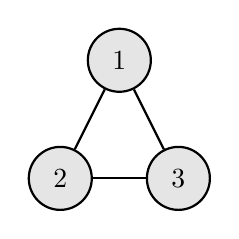
\begin{tikzpicture}
[every node/.style={draw, circle, fill=gray!20!, minimum size=8mm},
thick]
\node{1}
child{node(0){2}}
child{node(1){3}};
\draw (0)--(1);
\end{tikzpicture}
\end{figure}
\end{flushleft}

\paragraph{Example 2:}
\begin{flushleft}


\textbf{Input}: \lstinline[language=C++, basicstyle=\small\ttfamily, keywordstyle=\bfseries\color{green!40!black}]|[[1,2], [2,3], [3,4], [1,4], [1,5]]|

\textbf{Output}: \lstinline[language=C++, basicstyle=\small\ttfamily, keywordstyle=\bfseries\color{green!40!black}]|[1,4]|

\textbf{Explanation}: The given undirected graph will be like this:
\begin{figure}[H]
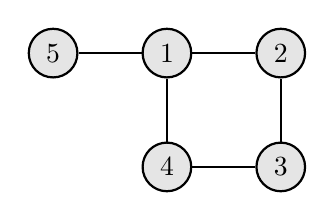
\begin{tikzpicture}
[every node/.style={draw, circle, fill=gray!20!, minimum size=5mm},
thick]
\node(0){5};
\node[right=8mm of 0](1){1};
\node[right=8mm of 1](2){2};
\node[below=8mm of 1](4){4};
\node[below=8mm of 2](3){3};
\draw (0) -- (1);
\draw (1) -- (2);
\draw (1) -- (4);
\draw (2) -- (3);
\draw (4) -- (3);
\end{tikzpicture}
\end{figure}
\end{flushleft}

\paragraph{Note:}
\begin{itemize}
\item The size of the input 2D-array will be between 3 and 1000.
\item Every integer represented in the 2D-array will be between 1 and $N$, where $N$ is the size of the input array.
\end{itemize}

\subsection{DFS}
题目的主要意图是在tree中检测出cycle。

We will detect cycle in the process of building adjacent list. For each edge $(u,v)$, we run a depth first search if there already exist a path from $u$ to $v$ before inserting $(u,v)$ into the adjacent list. Since this is a undirected graph, we don't need to search a path from $v$ to $u$.

The process of searching cycle is trivial: we first check if $v$ is already be a adjacent node of $u$. If it is not, we recursively deep into the adjacent nodes of $u$ to check. In this process, we must not consider the nodes we have already visited by adding current visit node number as the recursive function parameter.

\setcounter{lstlisting}{0}
\begin{lstlisting}[style=customc, caption={DFS}]
vector<int> findRedundantConnection( vector<vector<int>>& edges )
{
    vector<unordered_set<int>> adj( edges.size() + 1 );

    //build ajacent list
    for( const auto& edge : edges )
    {
        //if there is already a path
        //from edge[0] to edge[1]
        //there is a cycle
        if( dfs( edge[0], edge[1], adj, -1 ) )
        {
            return edge;
        }

        //since this is a undirected graph
        //we need to add both into their adjacent list
        adj[edge[0]].insert( edge[1] );
        adj[edge[1]].insert( edge[0] );
    }

    return {};
}

bool dfs( int start, int end, vector<unordered_set<int>>& G, int pre )
{
    //if end is the adjacent node of start
    //we found the path
    if( G[start].find( end ) != G[start].end() )
    {
        return true;
    }

    for( int next : G[start] )
    {
        //avoid visit
        //nodes that have been visited
        if( next == pre )
        {
            continue;
        }

        if( dfs( next, end, G, start ) )
        {
            return true;
        }
    }

    return false;
}
\end{lstlisting}

\subsection{Union Find}
For each edge $(u,v)$, we first find the parents of $u$ and $v$, say $p_u$ and $p_v$. If $p_u=p_v$, we know there already a path between $u$ and $v$ except direct edge $(u,v)$, i.e. a cycle. Otherwise, we set parent of $p_u$ to $p_v$ (set parent of $p_v$ to $p_u$ can also work).

\begin{lstlisting}[style=customc, caption={Union Find}]
vector<int> findRedundantConnection( vector<vector<int>>& edges )
{
    int N = static_cast<int>( edges.size() + 1 );

    vector<int> parents( N + 1, 0 );

    for( int i = 1; i <= N; ++i )
    {
        parents[i] = i;
    }

    for( const auto& edge : edges )
    {
        int p0 = find( parents, edge[0] );
        int p1 = find( parents, edge[1] );

        if( p0 == p1 )
        {
            //a path except current edge
            //exists between edge[0] and edge[1]
            //a cycle detected
            return edge;
        }

        //set parent of edge[0]
        //to parent of edge[1]
        parents[p0] = p1;
    }

    return {};
}

int find( vector<int>& parents, int x )
{
    while( x != parents[x] )
    {
        x = parents[x];
    }

    return x;
}
\end{lstlisting}
\section{685 --- Redundant Connection II}
In this problem, a rooted tree is a \textbf{directed} graph such that, there is exactly one node (the root) for which all other nodes are descendants of this node, plus every node has exactly one parent, except for the root node which has no parents.

The given input is a directed graph that started as a rooted tree with $ N $ nodes (with distinct values $ 1, 2, \ldots, N $), with one additional directed edge added. The added edge has two different vertices chosen from 1 to $ N $, and was not an edge that already existed.

The resulting graph is given as a 2D-array of edges. Each element of edges is a pair $ [u, v] $ that represents a directed edge connecting nodes $ u $ and $ v $, where $ u $ is a parent of child $ v $.

Return an edge that can be removed so that the resulting graph is a rooted tree of $ N $ nodes. If there are multiple answers, return the answer that occurs last in the given 2D-array.

\paragraph{Example 1:}

\begin{flushleft}
Input: \lstinline[language=C++, basicstyle=\small\ttfamily, keywordstyle=\bfseries\color{green!40!black}]|[[1,2], [1,3], [2,3]]|

Output: \lstinline[language=C++, basicstyle=\small\ttfamily, keywordstyle=\bfseries\color{green!40!black}]|[2,3]|

Explanation: The given directed graph will be like this:

\begin{figure}[H]
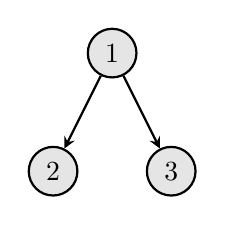
\begin{tikzpicture}
[every node/.style={draw, circle, fill=gray!20!, minimum size=5mm},
thick, >=stealth, ->]
\node{1}
child{node{2}}
child{node{3}};
\end{tikzpicture}
\end{figure}

\end{flushleft}

%  1
% / \
%v   v
%2-->3

\paragraph{Example 2:}
\begin{flushleft}


\textbf{Input}: \lstinline[language=C++, basicstyle=\small\ttfamily, keywordstyle=\bfseries\color{green!40!black}]|[[1,2], [2,3], [3,4], [4,1], [1,5]]|

\textbf{Output}: \lstinline[language=C++, basicstyle=\small\ttfamily, keywordstyle=\bfseries\color{green!40!black}]|[4,1]|

\textbf{Explanation}: The given directed graph will be like this:
\begin{figure}[H]
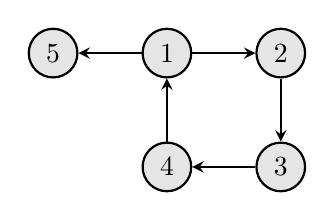
\begin{tikzpicture}
[every node/.style={draw, circle, fill=gray!20!, minimum size=5mm},
>=stealth, ->, thick]
\node(5){5};
\node[right=8mm of 5](1){1};
\node[right=8mm of 1](2){2};
\node[below=8mm of 1](4){4};
\node[below=8mm of 2](3){3};
\draw (1) -- (5);
\draw (1) -- (2);
\draw (4) -- (1);
\draw (2) -- (3);
\draw (3) -- (4);
\end{tikzpicture}
\end{figure}
\end{flushleft}
%5 <- 1 -> 2
%     ^    |
%     |    v
%     4 <- 3
\paragraph{Note:}

\begin{itemize}
\item The size of the input 2D-array will be between 3 and 1000.
\item Every integer represented in the 2D-array will be between 1 and $ N $, where $ N $ is the size of the input array.
\end{itemize}

\subsection{Union Find}
There are three cases in which a redundant edge exists.

\begin{enumerate}
\item No loop but there is a node with in-degree equal to 2. For example, 3 is the node in the following picture
\begin{figure}[H]
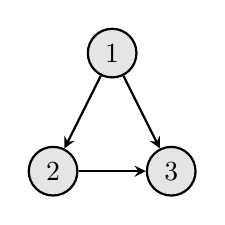
\begin{tikzpicture}
[every node/.style={draw, circle, fill=gray!20!, minimum size=5mm},
>=stealth, ->,thick]
\node{1}
child{node(2){2}}
child{node(3){3}};
\draw (2) -- (3);
\end{tikzpicture}
\end{figure}
\item A loop exists. All nodes have in-degree 1 or 0. as following example

\begin{figure}[H]
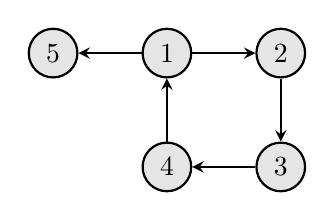
\begin{tikzpicture}
[every node/.style={draw, circle, fill=gray!20!, minimum size=5mm},
>=stealth, ->, thick]
\node(5){5};
\node[right=8mm of 5](1){1};
\node[right=8mm of 1](2){2};
\node[below=8mm of 1](4){4};
\node[below=8mm of 2](3){3};
\draw (1) -- (5);
\draw (1) -- (2);
\draw (4) -- (1);
\draw (2) -- (3);
\draw (3) -- (4);
\end{tikzpicture}
\end{figure}

\item A loop exists and one node has one in-degree 2. An example is shown as below

\begin{figure}[H]
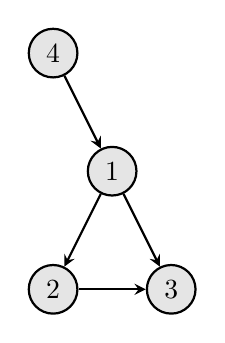
\begin{tikzpicture}
[every node/.style={draw, circle, fill=gray!20!, minimum size=5mm},
>=stealth, ->, thick]
\node{4}
child[missing]
child{node{1} child{node(2){2}} child{node(3){3}}};
\draw (2) -- (3);
\end{tikzpicture}
\end{figure}

\end{enumerate}

We process these 3 cases differently. 

\begin{itemize}
\item For the first case, we return the edge that has the node with in-degree 2 (i.e, $(2,3)$ in the example). 

\item To the 2nd case, we return the edge that form the loop (i.e., $(4,1)$ in the example.)

\item In the 3rd case, we return the edge that form the loop and contains the node with in-degree 2 (i.e., $(3,1)$ in the example).
\end{itemize}


We make use of an array $P$. For an edge $(u,v)$, this is $u\to v$, so $P[v]=u$. Initially all elements in $P$ are set to $-1$.

We start by looking for the node with in-degree equal to 2. Iterate the given edges array, for current edge $(u, v)$, if $P[v] \geq 0$, node $v$ will be the node with in-degree equal to 2. We save both previous edge $(P[v], v)$ and current edge $(u,v)$ as $e_1$ and $e_2$.

Next, we searching for loop using union find by traversing input edges again. Whenever we find a loop, we will check if $e_0$ exists or not. If $e_0$ does exist, we just return $e_0$ (case 3). Otherwise, we return current edge which forms a loop (case 2).

Finally, if we don't return during the traversing, we will return $e_2$ (case 1).

\setcounter{lstlisting}{0}
\begin{lstlisting}[style=customc, caption={Union Find}]
vector<int> findRedundantDirectedConnection( vector<vector<int>>& edges )
{
    int N = static_cast<int>( edges.size() );

    vector<int> parents( N + 1, 0 );

    vector<int> e1;
    vector<int> e2;

    //check node with in-degree 2
    for( auto& edge : edges )
    {
        int src = edge[0];
        int dst = edge[1];

        if( parents[dst] == 0 )
        {
            parents[dst] = src;
        }
        else
        {
            //dst has in-degree 2
            //save previous edge and current edge
            e1.assign( {parents[dst], dst} );

            e2 = edge;

            //invalidate edge
            edge[1] = -1;
        }
    }

    //check for loop
    for( int i = 1; i <= N; ++i )
    {
        parents[i] = i;
    }

    for( const auto& edge : edges )
    {
        if( edge[1] < 0 )
        {
            continue;
        }

        int p0 = find( parents, edge[0] );
        int p1 = find( parents, edge[1] );

        if( p0 == p1 )
        {
            //loop
            if( e1.empty() )
            {
                return edge; //case 2
            }
            else
            {
                return e1; //case 3
            }
        }

        //link edge[0] and edge[1]
        parents[p1] = p0;
    }

    //case 1
    return e2;
}

int find( vector<int>& parents, int x )
{
    while( parents[x] != x )
    {
        x = parents[x];
    }

    return x;
}
\end{lstlisting}



\section{686 --- Repeated String Match}
Given two strings $A$ and $B$, find the minimum number of times $A$ has to be repeated such that $B$ is a substring of it. If no such solution, return $-1$.

For example, with \lstinline[language=C++, basicstyle=\small\ttfamily, keywordstyle=\bfseries\color{green!40!black}]|A = "abcd"| and \lstinline[language=C++, basicstyle=\small\ttfamily, keywordstyle=\bfseries\color{green!40!black}]|B = "cdabcdab"|.

Return 3, because by repeating $A$ three times (\lstinline[language=C++, basicstyle=\small\ttfamily, keywordstyle=\bfseries\color{green!40!black}]|"abcdabcdabcd"|), $B$ is a substring of it; and $B$ is not a substring of $A$ repeated two times (\lstinline[language=C++, basicstyle=\small\ttfamily, keywordstyle=\bfseries\color{green!40!black}]|"abcdabcd"|).

\paragraph{Note:}

\begin{itemize}
\item The length of $ A $ and $ B $ will be between 1 and 10000.
\end{itemize}

\subsection{Sliding Window}
We keep track of index $i$ and $j$ for $A$ and $B$, then compare $A[i]$ with $B[j]$. Since $A$ can repeat, the index that we will scanning in $A$ will be $\bmod(i+j, L_A)$ where $L_A$ is the length of $A$.

We increments $j$ whenever $A[\bmod(i+j, L_A)]=B[j]$ until the end of $B$. If $j=L_B$ ($L_B$ is the length of $B$), we know $B$ will appear as a substring in a string with repeated $A$. The count of repeat will be $(i+j-1)/L_A+1$. The reason is when $i+j=L_A$, the count of repeating $A$ is 1.

\setcounter{lstlisting}{0}
\begin{lstlisting}[style=customc, caption={Sliding Window}]
int repeatedStringMatch( string A, string B )
{
    size_t LA = A.size();

    size_t LB = B.size();

    for( size_t i = 0; i < LA; ++i )
    {
        size_t  j = 0;

        while( j < LB )
        {
            //we start from (i+j) % LA
            auto k = ( i + j ) % LA;

            if( A[k] == B[j] )
            {
                ++j;
            }
            else
            {
                break;
            }
        }

        //all are matched
        //LB is the substring
        if( j == LB )
        {
            return ( i + j - 1 ) / LA + 1;
        }
    }

    return -1;
}
\end{lstlisting}

\subsection{KMP}
We build a KMP table $T$ for string $B$. The comparing scheme is same as the sliding window approach, i.e.

\begin{lstlisting}[style=customc, caption={Scanning Scheme}]
while( j < LB )
{
    //we start from (i+j) % LA
    //when j is incremented
    //i+j is also incremented
    //because i is fixed.
    auto k = ( i + j ) % LA;

    if( A[k] == B[j] )
    {
        ++j;
    }
    else
    {
        break;
    }
}
\end{lstlisting}

When the matching is failed at some index $j$, we will utilize the KMP table to find the next matching index. In this problem, since the index to scan in $A$, $i$, is fixed when comparing, $i$ will be changed to $i + j - T[j-1]$. (In the normal string matching KMP, the scanning index $i$ in the string to be searched is incremented when matched).


\begin{lstlisting}[style=customc, caption={KMP}]
int repeatedStringMatch( string A, string B )
{
    auto LA = static_cast< int >( A.size() );
    auto LB = static_cast< int >( B.size() );

    //build KMP table
    vector<int> F( B.size(), 0 );
    int t = 0;
    for( int i = 1; i < LB; ++i )
    {
        t = F[i - 1];

        while( ( t > 0 ) && ( B[i] != B[t] ) )
        {
            t = F[t - 1];

        }

        if( B[i] == B[t] )
        {
            t = t + 1;
        }

        F[i] = t;
    }

    int i = 0; //index in A
    int j = 0; //index in B

    while( i < LA )
    {
        while( j < LB )
        {
            //during this process
            //i is fixed
            //(i+j) is incremented

            auto k = ( i + j ) % LA;
            if( A[k] == B[j] )
            {
                ++j;

            }
            else
            {
                break;
            }
        }


        if( j == LB )
        {
            //found match
            return ( i + j - 1 ) / LA + 1;
        }


        if( j > 0 )
        {
            //since i is fixed during comparing
            //we need to advance i to the
            //first index that does not match
            //which is i + j - F[j-1]

            //In normal KMP, since i is
            //incremented during comparing
            //the following is not needed
            i += j - F[j - 1];

            //normal KMP operation
            j = F[j - 1];
        }
        else
        {
            //same as normal KMP operation
            ++i;
        }

    }
    return -1;
}
\end{lstlisting}

\section{687 --- Longest Univalue Path}
Given a binary tree, find the length of the longest path where each node in the path has the same value. This path may or may not pass through the root.

The length of path between two nodes is represented by the number of edges between them.

 

\paragraph{Example 1:}

\begin{flushleft}
\textbf{Input}:

\begin{figure}[H]
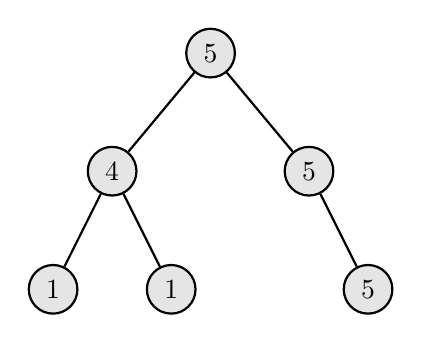
\begin{tikzpicture}
[every node/.style={draw, circle, fill=gray!20!, minimum size=5mm},
level 1/.style={sibling distance=25mm},
level 2/.style={sibling distance=15mm},
thick]
\node{5}
child{node{4} child{node{1}} child{node{1}} }
child{node{5} child[missing] child{node{5}}};
\end{tikzpicture}
\end{figure}

\textbf{Output}: 2

 
\end{flushleft}

\paragraph{Example 2:}

\begin{flushleft}
\textbf{Input}:

\begin{figure}[H]
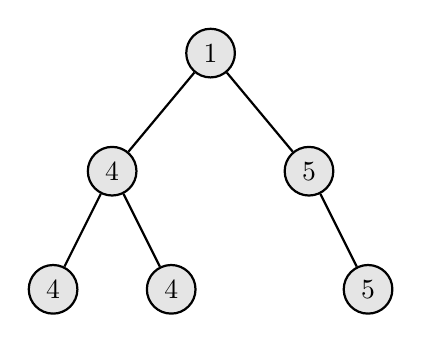
\begin{tikzpicture}
[every node/.style={draw, circle, fill=gray!20!, minimum size=5mm},
level 1/.style={sibling distance=25mm},
level 2/.style={sibling distance=15mm},
thick]
\node{1}
child{node{4} child{node{4}} child{node{4}} }
child{node{5} child[missing] child{node{5}}};
\end{tikzpicture}
\end{figure}


\textbf{Output}: 2
\end{flushleft}

 

\paragraph{Note: }
\begin{itemize}
\item The given binary tree has not more than 10000 nodes. The height of the tree is not more than 1000.
\end{itemize}

\subsection{Recursion}
Suppose $l$ and $r$ are the length of two longest path which are starting from current node's left and right child respectively.

Similar to the problem that finding the path sum of the tree, the recursive function will return the longest path that is from current node, and the length of the global longest path will be the parameter of the function.

When current node's value is equal to left child's value, we extend $l$ to $l+1$ because the path can extend to current node, otherwise set $l$ to 0.

Similarly, we extend $r$ to $r+1$ when right child and current node have same values, otherwise, set $r$ to 0.

Then, we update global maximum length as maximum of itself and ($l+r$).

\setcounter{lstlisting}{0}
\begin{lstlisting}[style=customc, caption={Recursion}]
int longestUnivaluePath( TreeNode* root )
{
    int ans = 0;

    dfs( root, ans );

    return ans;
}

int dfs( TreeNode* node, int& ans )
{
    if( !node )
    {
        return 0;
    }

    int left = dfs( node->left, ans );

    int from_left = 0;

    if( node->left )
    {
        if( node->left->val == node->val )
        {
            //extend left length
            from_left = left + 1;
        }
    }

    int right = dfs( node->right, ans );
    int from_right = 0;
    if( node->right )
    {
        if( node->right->val == node->val )
        {
            //extend right length
            from_right = right + 1;
        }
    }

    //return maximum of left and right
    int ret = ( max )( from_left, from_right );
    //update global maximum
    ans = ( max )( ans, from_left + from_right );

    return ret;
}
\end{lstlisting}
\section{688 --- Knight Probability in Chessboard}
On an $N\times N$ chessboard, a knight starts at the $r$-th row and $c$-th column and attempts to make exactly $K$ moves. The rows and columns are 0 indexed, so the top-left square is $(0, 0)$, and the bottom-right square is $(N-1, N-1)$.

A chess knight has 8 possible moves it can make. Each move is two squares in a cardinal direction, then one square in an orthogonal direction.
 
Each time the knight is to move, it chooses one of eight possible moves uniformly at random (even if the piece would go off the chessboard) and moves there.

The knight continues moving until it has made exactly K moves or has moved off the chessboard. Return the probability that the knight remains on the board after it has stopped moving.
 

\paragraph{Example:}

\begin{flushleft}
\textbf{Input}: 3, 2, 0, 0

\textbf{Output}: 0.0625

\textbf{Explanation}: 

There are two moves (to \lstinline[language=C++, basicstyle=\small\ttfamily, keywordstyle=\bfseries\color{green!40!black}]|(1,2), (2,1)|) that will keep the knight on the board.

From each of those positions, there are also two moves that will keep the knight on the board.

The total probability the knight stays on the board is 0.0625.
\end{flushleft}


  

\paragraph{Note:}

\begin{itemize}
\item $N$ will be between 1 and 25.

\item $K$ will be between 0 and 100.

\item The knight always initially starts on the board.
\end{itemize}

\subsection{Dynamic Programming}
Suppose $F[i][j][x]$ be the probability of being on square $(i,j)$ after $x$ steps. Based on how a knight moves, we have the following recursion:

$F[i][j][x] = \sum\limits_{i=1}^{8}F[i+\delta_i][j+\delta_j][x-1] / 8$

where $(\delta_i, \delta_j)$ is from one of 

$(2, 1)$, $(2,1)$, $ (2, -1) $, $ (2,−1) $, 

$ (-2, 1) $, $ (−2,1) $, $ (-2, -1) $, $ (−2,−1) $, 

$ (1, 2) $, $ (1,2) $, $ (1, -2) $, $ (1,−2) $, 

$ (-1, 2) $, $ (−1,2) $, $ (-1, -2) $, $ (−1,−2) $.

We can make use of two 2d array: $F_0$ and $F_1$ instead of 3-D array.

\setcounter{lstlisting}{0}
\begin{lstlisting}[style=customc, caption={Dynamic Programming}]
double knightProbability( int N, int K, int r, int c )
{
    //the next 8 jumps for knight
    int dr[] = { 2, 2, 1, 1, -1, -1, -2, -2 };
    int dc[] = { 1, -1, 2, -2, 2, -2, 1, -1 };

    vector<vector<double>> F( N, vector<double>( N, 0 ) );
    vector<vector<double>> Next( N, vector<double>( N, 0 ) );

    //at start, the probability is one
    F[r][c] = 1;

    for( int i = 1; i <= K; ++i )
    {
        for( int r = 0; r < N; ++r )
        {
            for( int c = 0; c < N; ++c )
            {
                for( int x = 0; x < 8; ++x )
                {
                    int nr = r + dr[x];
                    int nc = c + dc[x];

                    if( ( nr >= 0 ) && ( nr < N ) && ( nc >= 0 ) && ( nc < N ) )
                    {
                        //(nr,nc) is the next square from (r,c)
                        //it could jump from 7 other squares.
                        //so we add the probability of F[r][c]/8
                        Next[nr][nc] += F[r][c] / 8;
                    }
                }
            }//end c
        }//end r

        swap( F, Next );

        //reset Next to zeros
        for( auto& v : Next )
        {
            fill( v.begin(), v.end(), 0 );
        }

    }//end i

    //the total sum of F
    //will be the answer
    double ans = 0;

    for( const auto& v : F )
    {
        ans += accumulate( v.begin(), v.end(), 0.0 );
    }

    return ans;
}
\end{lstlisting}
\section{689 --- Maximum Sum of 3 Non-Overlapping Subarrays}
In a given array $A$ of positive integers, find three non-overlapping subarrays with maximum sum.

Each subarray will be of size $k$, and we want to maximize the sum of all $3k$ entries.

Return the result as a list of indices representing the starting position of each interval (0-indexed). If there are multiple answers, return the lexicographically smallest one.

\paragraph{Example:}

\begin{flushleft}
\textbf{Input}: \lstinline[language=C++, basicstyle=\small\ttfamily, keywordstyle=\bfseries\color{green!40!black}]|[1,2,1,2,6,7,5,1]|,  $k=2$

\textbf{Output}: \lstinline[language=C++, basicstyle=\small\ttfamily, keywordstyle=\bfseries\color{green!40!black}]|[0, 3, 5]|

Explanation: Subarrays \lstinline[language=C++, basicstyle=\small\ttfamily, keywordstyle=\bfseries\color{green!40!black}]|[1, 2], [2, 6], [7, 5]| correspond to the starting indices \lstinline[language=C++, basicstyle=\small\ttfamily, keywordstyle=\bfseries\color{green!40!black}]|[0, 3, 5]|.

We could have also taken \lstinline[language=C++, basicstyle=\small\ttfamily, keywordstyle=\bfseries\color{green!40!black}]|[2, 1]|, but an answer of \lstinline[language=C++, basicstyle=\small\ttfamily, keywordstyle=\bfseries\color{green!40!black}]|[1, 3, 5]| would be lexicographically larger.
\end{flushleft}
 

\paragraph{Note:}

\begin{itemize}
\item Size of $A$ will be between 1 and 20000.
\item $A[i]$ will be between 1 and 65535.
\item $k$ will be between 1 and $\lfloor \lvert A\rvert\ /3 \rfloor$.
\end{itemize}

\subsection{Dynamic Programming}
Suppose we have an array $W$, where each $W[s]$ represents sum of interval $A[s, s+K-1]$. To create $W$, we can either use prefix sums, or manage the sum of the interval as a window slides along the array.

Then, we have a reduced problem: Given array $W$ and an integer $K$, what is the lexicographically smallest tuple of indices $(x, y, z)$ with $x + K <\leq y$ and $y + K \leq z$ that maximizes $W[x] + W[y] + W[z]$ ?

Suppose we fixed $y$. We would like to know on the intervals $x \in [0, y-K]$ and $z \in [j+K, \lvert W\rvert-1$, where the largest value of $W[x]$ (and respectively $W[z]$) occurs first. (Here, \textbf{first} means the smaller index.)

We can solve these problems with dynamic programming. We make use of two arrays $B$ and $E$ where

\begin{enumerate}
\item Each $B[i]$ stores the first index of the largest of $W[x]$ for $x \in [0, i]$, and 
\item Each $E[j]$ stores the first index of the largest of $W[z]$ for $z \in [j, \lvert W\rvert - 1]$.
\end{enumerate}

This means that for some choice $y$, the candidate must be $(B[y-K], y, E[j+K])$. We take the candidate that produces the maximum $W[x] + W[y] + W[z]$.

\setcounter{lstlisting}{0}
\begin{lstlisting}[style=customc, caption={Dynamic Programming}]
vector<int> maxSumOfThreeSubarrays( vector<int>& nums, int k )
{
    //fill S that record each interval's sum
    int N = static_cast<int>( nums.size() );

    vector<int> S( N - k + 1, 0 );

    int sum = 0;

    for( int i = 0; i < N; ++i )
    {
        sum += nums[i];

        if( i >= k )
        {
            sum -= nums[i - k];
        }

        if( i >= k - 1 )
        {
            S[i - k + 1] = sum;
        }
    }

    //make array B
    //which records the first index
    //of maximum S from left to right
    int nS = N - k + 1;
    int best = 0;
    vector<int> B( nS );
    for( int x = 0; x < nS; ++x )
    {
        if( S[x] > S[best] )
        {
            best = x;
        }

        B[x] = best;
    }

    //make array E
    //which record the first index
    //of maximum S from right to left

    best = nS - 1;
    vector<int> E( nS );
    for( int z = nS - 1; z >= 0; --z )
    {
        //since this is from right to left
        //and we need first occurence
        //we also need update when the S[z] = S[best]
        if( S[z] >= S[best] )
        {
            best = z;
        }

        E[z] = best;
    }

    //find out best tuple (x,y,z) which can make
    //largest S[x]+S[y]+S[z]

    vector<int> ans {0, k, k + k};
    int max3S = S[ans[0]] + S[ans[1]] + S[ans[2]];
    for( int y = k; y < nS - k; ++y )
    {
        int x = B[y - k]; //x <=y-k
        int z = E[y + k]; //z >= y+k

        int total = S[x] + S[y] + S[z];

        if( total > max3S )
        {
            ans.assign( {x, y, z} );
            max3S = total;
        }
    }

    return ans;
}
\end{lstlisting}
\section{690 --- Employee Importance}

\textbf{Easy}

You are given a data structure of employee information, which includes the employee's \textbf{unique id}, his \textbf{importance} value and his \textbf{direct} subordinates' id.

For example, employee 1 is the leader of employee 2, and employee 2 is the leader of employee 3. They have importance value 15, 10 and 5, respectively. Then employee 1 has a data structure like \fcj{[1, 15, [2]]}, and employee 2 has \fcj{[2, 10, [3]]}, and employee 3 has \fcj{[3, 5, []]}. Note that although employee 3 is also a subordinate of employee 1, the relationship is not direct.

Now given the employee information of a company, and an employee id, you need to return the total importance value of this employee and all his subordinates.

\paragraph{Example 1:}

\begin{flushleft}
\textbf{Input}: \fcj{[[1, 5, [2, 3]], [2, 3, []], [3, 3, []]]}, 1

\textbf{Output}: 11

\textbf{Explanation}:

Employee 1 has importance value 5, and he has two direct subordinates: employee 2 and employee 3. They both have importance value 3. So the total importance value of employee 1 is $5 + 3 + 3 = 11$.
\end{flushleft}
 

\paragraph{Note:}

\begin{itemize}
\item One employee has at most one direct leader and may have several subordinates.

\item The maximum number of employees won't exceed 2000.
\end{itemize}

\subsection{DFS}
We need a hash map which map a employee's id to itself. Then we make use of DFS to recursively get all the subordinates of the given id.

\setcounter{lstlisting}{0}
\begin{lstlisting}[style=customc, caption={DFS}]
int getImportance( vector<Employee*> employees, int id )
{
    unordered_map<int, Employee*> m;
    //build the map between id and Employee
    for( auto p : employees )
    {
        m[p->id] = p;
    }
    return dfs( id, m );
}
int dfs( int id, const unordered_map<int, Employee*>& m )
{
    //recursively get the
    //total importance values of
    //all subordinates of id
    auto p = m[id];
    int sum = p->importance;
    for( int id : p->subordinates() )
    {
        sum += dfs( id, m );
    }
    return sum;
}
\end{lstlisting}

\paragraph{Related Problems}
\begin{itemize}
\item \textbf{339. Nested List Weight Sum}.
\end{itemize}
\section{691 --- Stickers to Spell Word}
We are given $N$ different types of \textbf{stickers}. Each sticker has a \textbf{lowercase} English word on it.
\par
You would like to spell out the given \textbf{target} string $T$ by cutting individual letters from your collection of stickers and rearranging them.
\par
You can use each sticker more than once if you want, and you have infinite quantities of each sticker.
\par
What is the minimum number of stickers that you need to spell out the target? If the task is impossible, return -1.
\paragraph{Example 1:}
\begin{flushleft}
\textbf{Input:}

\lstinline[language=C++, basicstyle=\small\ttfamily, keywordstyle=\bfseries\color{green!40!black}]|stickers = ["with", "example", "science"]|, \lstinline[language=C++, basicstyle=\small\ttfamily, keywordstyle=\bfseries\color{green!40!black}]|target = "thehat"|.

\textbf{Output}: 3

\textbf{Explanation}:

We can use 2 \lstinline[language=C++, basicstyle=\small\ttfamily, keywordstyle=\bfseries\color{green!40!black}]|"with"| stickers, and 1 \lstinline[language=C++, basicstyle=\small\ttfamily, keywordstyle=\bfseries\color{green!40!black}]|"example"| sticker.

After cutting and rearrange the letters of those stickers, we can form the target \lstinline[language=C++, basicstyle=\small\ttfamily, keywordstyle=\bfseries\color{green!40!black}]|"thehat"|.

Also, this is the minimum number of stickers necessary to form the target string.
\end{flushleft}

\paragraph{Example 2:}
\begin{flushleft}
\textbf{Input}:

\lstinline[language=C++, basicstyle=\small\ttfamily, keywordstyle=\bfseries\color{green!40!black}]|stickers=["notice", "possible"]|, \lstinline[language=C++, basicstyle=\small\ttfamily, keywordstyle=\bfseries\color{green!40!black}]|target = "basicbasic"|

\textbf{Output}: $-1$

\textbf{Explanation}:

We can't form the target \lstinline[language=C++, basicstyle=\small\ttfamily, keywordstyle=\bfseries\color{green!40!black}]|"basicbasic"| from cutting letters from the given stickers.
\end{flushleft}


\paragraph{Note:}
\begin{itemize}
\item \textbf{stickers} has length in the range $[1, 50]$.
\item \textbf{stickers} consists of \textbf{lowercase} English words (without apostrophes).
\item \textbf{target} has length in the range $[1, 15]$, and consists of \textbf{lowercase} English letters.
\item In all test cases, all words were chosen randomly from the 1000 most common US English words, and the target was chosen as a concatenation of two random words.
\item The time limit may be more challenging than usual. It is expected that a 50 sticker test case can be solved within 35ms on average.
\end{itemize}

\subsection{Dynamic Programming}
In this approach, suppose the length of $T$ is $L$. Since the given $L$ is no large than 15, we can make use of a integer $s$  such that if the $i$--th bit of $s$ is 1, it means $T[i]$ can be spelled by the sticker. 


For each state $s$, we look at what happens to it after applying a sticker. For each letter in the sticker that can satisfy an unset bit of $s$, we set the bit. At the end, we know now is the result of applying that sticker to state. 

Thus, we make use of an array $F$. For each state $s$, $F[s]$ gives the minimum number of stickers such that: for each set bit $i$ in $s$, $T[i]$ can be spelled by the stickers. 

We starting from zero state. For each current state $s$, we apply a sticker and will get next state $s_1$. Then $F[s_1]=\min(F[s_1], F[s]+1)$. After checking all $2^L$ states, $F[2^L-1]$ is the answer.

\subsubsection{Algorithm}
The inputs of the following procedure are
\begin{itemize}
    \item $S$ --- The input sticker array
    \item $N$ --- The length of $S$
    \item $T$ --- The target string
    \item $L$ --- The length of $T$
\end{itemize}

\setcounter{lstlisting}{0}
\begin{lstlisting}[style=customc, caption={Dynamic Progamming}]
int minStickers( vector<string>& stickers, string target )
{
    int L = static_cast<int>( target.size() );
    //the space of states
    int NS = ( 1 << L );

    vector<int> F( NS, -1 );
    //at start, all bits are 0
    //no any sticker is needed
    F[0] = 0;

    //try each state
    for( int state = 0; state < NS; ++state )
    {
        if( F[state] < 0 )
        {
            //this state cannot
            //be reached
            continue;
        }

        for( const auto& sticker : stickers )
        {
            //apply one sticker to
            //current state
            //to get next_state
            int next_state = state;

            for( auto ch : sticker )
            {
                for( size_t i = 0; i < target.size(); ++i )
                {
                    if( next_state & ( 1 << i ) )
                    {
                        //we already spell out target[i]
                        continue;
                    }
                    if( target[i] == ch )
                    {
                        //we can spell letter target[i]
                        next_state |= ( 1 << i );
                        //we try next letter in the sticker
                        break;
                    }
                }//loop target
            }//loop letter in sticker

            //now next_state is the result of applying the sticker
            if( ( F[next_state] < 0 ) || ( F[next_state] > F[state] + 1 ) )
            {
                //the number of stickers
                //for reach next_state
                //is the number of stickers
                //to reach state plus 1
                F[next_state] = F[state] + 1;
            }
        }// loop stickers
    }//loop state

    return F.back();
}
\end{lstlisting}
\section{692 --- Top K Frequent Words}
Given a non-empty list of words, return the $k$ most frequent elements.

Your answer should be sorted by frequency from highest to lowest. If two words have the same frequency, then the word with the lower alphabetical order comes first.

\paragraph{Example 1:}

\begin{flushleft}
\textbf{Input}: 

\fcc{["i", "love", "leetcode", "i", "love", "coding"]}, 

$k = 2$

\textbf{Output}: \fcc{["i", "love"]}

\textbf{Explanation}: \fcc{"i"} and \fcc{"love"} are the two most frequent words.

Note that \fcc{"i"} comes before \fcc{"love"} due to a lower alphabetical order.
\end{flushleft}

\paragraph{Example 2:}

\begin{flushleft}
\textbf{Input}: 

\fcc{["the", "day", "is", "sunny", "the", "the", "the", "sunny", "is", "is"]}, 

$k = 4$

\textbf{Output}: \fcc{["the", "is", "sunny", "day"]}

\textbf{Explanation}: 

\fcc{"the"}, \fcc{"is"}, \fcc{"sunny"} and \fcc{"day"} are the four most frequent words, with the number of occurrence being 4, 3, 2 and 1 respectively.
\end{flushleft}

\paragraph{Note:}

\begin{itemize}
\item You may assume $ k $ is always valid, $1 \leq k \leq N$, where $N$ is number of unique elements.
\item Input words contain only lowercase letters.
\end{itemize}

\paragraph{Follow up:}

\begin{itemize}
\item Try to solve it in $ O(n log k) $ time and $ O(n) $ extra space.
\end{itemize}

\subsection{Heap}
This is a typical heap structure (priority queue) usage problem. When using \fcc{"C++ priority_queue"}, the ordering is defined as below
\begin{itemize}
\item The word with less appearances are put on the top of the queue.
\item If two words have same appearances, put the higher alphabetical order word on the top of the queue
\end{itemize}

We can lower the memory usage by using 

\fcc{"class string_view"}, 

and we can directly use the \fcc{"iterator"} of the hash map as the element of the queue.

\setcounter{lstlisting}{0}
\begin{lstlisting}[style=customc, caption={Heap}]
vector<string> topKFrequent( vector<string>& words, int k )
{
    using dict_type = unordered_map<string_view, int>;

    dict_type dict;

    //first count the appearances of each word
    for( const auto& word : words )
    {
        string_view sv( word );

        dict[word] += 1;
    }

    auto cmp = []( dict_type::iterator it1, dict_type::iterator it2 )
    {
        if( it1->second > it2->second )
        {
            //the less appearances will
            //on the top
            return true;
        }

        if( it1->second == it2->second )
        {
            //the higher alphabetical order word
            //will on the top
            return it1->first < it2->first;
        }

        return false;
    };

    //use iterator as the element of the queue
    priority_queue<dict_type::iterator, vector<dict_type::iterator>, decltype( cmp )> pq( cmp );

    for( auto it = dict.begin(); it != dict.end(); ++it )
    {
        pq.push( it );

        int n = static_cast< int >( pq.size() );

        if( n > k )
        {
            //remove the top
            pq.pop();
        }
    }

    vector<string> ans;
    ans.reserve( k );

    while( !pq.empty() )
    {
        auto it = pq.top();
        ans.emplace_back( it->first );
        pq.pop();
    }

    //since high alphabetical word is added first
    //we will reverse the result
    reverse( begin( ans ), end( ans ) );
    return ans;
}
\end{lstlisting}
\include{693}
\section{694 --- Number of Distinct Islands}
Given a non-empty 2D array grid of 0's and 1's, an island is a group of 1's (representing land) connected 4-directionally (horizontal or vertical.) You may assume all four edges of the grid are surrounded by water.

Count the number of distinct islands. An island is considered to be the same as another if and only if one island can be translated (and not rotated or reflected) to equal the other.

\paragraph{Example 1:}

\begin{flushleft}
\[
\begin{bmatrix}
1 & 1 & 0 & 0 & 0 \\
1 & 1 & 0 & 0 & 0 \\
0 & 0 & 0 & 1 & 1 \\
0 & 0 & 0 & 1 & 1
\end{bmatrix}
\]


Given the above grid map, return 1.

\end{flushleft}

\paragraph{Example 2:}

\begin{flushleft}
\[
\begin{bmatrix}
1 & 1 & 0 & 1 & 1\\
1 & 0 & 0 & 0 & 0\\
0 & 0 & 0 & 0 & 1\\
1 & 1 & 0 & 1 & 1
\end{bmatrix}
\]


Given the above grid map, return 3.

\end{flushleft}

\begin{flushleft}
Notice that:

\[
\begin{bmatrix}
1 & 1\\
1 &
\end{bmatrix}
\]

and

\[
\begin{bmatrix}
1 & \\
1 & 1\\
\end{bmatrix}
\]
\end{flushleft}

are considered different island shapes, because we do not consider reflection / rotation.

\paragraph{Note:} 

\begin{itemize}
\item The length of each dimension in the given grid does not exceed 50.
\end{itemize}

\subsection{Record Path Signature}

At the beginning, we need to find every island, which we can do using a straightforward depth-first search. 

Since two islands are the same if one can be translated to match another, let's translate every island so the top-left corner is \fcc{(0, 0)} For example, if an island is made from squares \fcc{[(2, 3), (2, 4), (3, 4)]}, we can think of this shape as \fcc{[(0, 0), (0, 1), (1, 1)]} when anchored at the top-left corner.

We can recording the path during the depth first search process and put it into a tree set.

As long as two regions are same, the offset coordinates for the points along the path will have same sequence when using same search directions. 

\setcounter{lstlisting}{0}
\begin{lstlisting}[style=customc, caption={Record Path}]
int numDistinctIslands( vector<vector<int>>& grid )
{
    auto M = grid.size();
    auto N = grid[0].size();

    int ans = 0;

    set<vector<int>> shapes;

    for( size_t r = 0; r < M; ++r )
    {
        for( size_t c = 0; c < N; ++c )
        {
            if( grid[r][c] == 1 )
            {
                //shape  record the path
                //during depth first search
                vector<int> shape;

                dfs( grid, r, c, r, c, shape );

                //add to set
                shapes.insert( shape );
            }
        }
    }

    return shapes.size();
}

//(r0,c0) is the starting point to depth first search
//which is the top left corner
//(because we can from top to bottom and left to right)
void dfs( vector<vector<int>>& G, int r0, int c0, int r, int c, vector<int>& shape )
{
    if( ( G[r][c] == 2 ) || ( G[r][c] == 0 ) )
    {
        return;
    }


    G[r][c] = 2;


    auto M = static_cast< int >( G.size() );
    auto N = static_cast< int >( G[0].size() );

    //get the offset per the left up corner (r0,c0)
    shape.push_back( ( r - r0 ) * N + ( c - c0 ) );

    int dr[] = { -1, 0, 1, 0 };
    int dc[] = { 0, -1, 0, 1 };

    for( int i = 0; i < 4; ++i )
    {
        int nr = r + dr[i];
        int nc = c + dc[i];

        if( ( nr >= 0 ) && ( nr < M ) && ( nc >= 0 ) && ( nc < N ) )
        {
            dfs( G, r0, c0, nr, nc, shape );
        }
    }
}
\end{lstlisting}


\section{695 --- Max Area of Island}
Given a non-empty 2D array grid of 0's and 1's, an island is a group of 1's (representing land) connected 4-direction (horizontal or vertical.) You may assume all four edges of the grid are surrounded by water.
\par
Find the \textbf{maximum area} of an island in the given 2D array. (If there is no island, the maximum area is 0.)
\paragraph{Example 1:}
\begin{flushleft}
\begin{figure}[H]
\centering
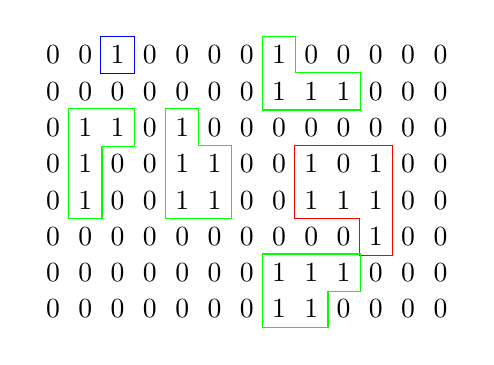
\begin{tikzpicture} 
\matrix (m) [matrix of nodes]
{
0 & 0 & 1 & 0 & 0 & 0 & 0 & 1 & 0 & 0 & 0 & 0 & 0 \\
0 & 0 & 0 & 0 & 0 & 0 & 0 & 1 & 1 & 1 & 0 & 0 & 0 \\
0 & 1 & 1 & 0 & 1 & 0 & 0 & 0 & 0 & 0 & 0 & 0 & 0 \\
0 & 1 & 0 & 0 & 1 & 1 & 0 & 0 & 1 & 0 & 1 & 0 & 0 \\
0 & 1 & 0 & 0 & 1 & 1 & 0 & 0 & 1 & 1 & 1 & 0 & 0 \\
0 & 0 & 0 & 0 & 0 & 0 & 0 & 0 & 0 & 0 & 1 & 0 & 0 \\
0 & 0 & 0 & 0 & 0 & 0 & 0 & 1 & 1 & 1 & 0 & 0 & 0 \\
0 & 0 & 0 & 0 & 0 & 0 & 0 & 1 & 1 & 0 & 0 & 0 & 0 \\
};
\draw [color=green](m-1-8.north west)--(m-2-8.south west)--(m-2-10.south east)--(m-2-10.north east)--(m-2-8.north east)--(m-1-8.north east)--cycle;
\draw [color=green](m-3-2.north west)--(m-5-2.south west)--(m-5-2.south east)--(m-3-2.south east)--(m-3-3.south east)--(m-3-3.north east)--cycle;
\draw [color=green](m-3-5.north west)--(m-5-5.south west)--(m-5-6.south east)--(m-4-6.north east)--(m-4-5.north east)--(m-3-5.north east)--cycle;
\draw [color=red](m-4-9.north west)--(m-5-9.south west)--(m-5-11.south west)--(m-6-11.south west)--(m-6-11.south east)--(m-4-11.north east)--cycle;
\draw [color=green](m-7-8.north west)--(m-8-8.south west)--(m-8-9.south east)--(m-7-9.south east)--(m-7-10.south east)--(m-7-10.north east)--cycle;
\draw [color=blue](m-1-3.north west)--(m-1-3.south west)--(m-1-3.south east)--(m-1-3.north east)--cycle;
\end{tikzpicture}
\end{figure}

Given the above grid, return 6. 

Note the answer is not 11, because the island must be connected 4-direction.
\end{flushleft}

\paragraph{Example 2:}
\begin{flushleft}
\[
\begin{bmatrix}
0 & 0 & 0 & 0 & 0 & 0 & 0 & 0
\end{bmatrix}
\]

Given the above grid, return 0.
\end{flushleft}

\paragraph{Note:}
\begin{itemize}
\item The length of each dimension in the given grid does not exceed 50.
\end{itemize}

\subsection{DFS}

很显然这时寻找四连通区域,在每一个1处进行DFS搜索,搜索完成后,即可获得当前连通区域中1的个数,也就是area大小。这里的一个技巧是,可以把访问到的元素设为$-1$,这样避免了使用额外的二维数组来记录是否访问过。

\setcounter{lstlisting}{0}
\begin{lstlisting}[style=customc, caption={DFS}]
int maxAreaOfIsland( vector<vector<int>>& grid )
{
    int M = static_cast< int >( grid.size() );
    int N = static_cast< int >( grid[0].size() );

    int best = 0;

    for( int r = 0; r < M; ++r )
    {
        for( int c = 0; c < N; ++c )
        {
            if( grid[r][c] == 1 )
            {
                int area = 0;

                dfs( grid, r, c, area );

                best = ( max )( area, best );
            }
        }
    }

    return best;
}

void dfs( vector<vector<int>>& G, int r, int c, int& area )
{
    if( G[r][c] != 1 )
    {
        return;
    }

    //this is a point we have not seen
    //and also belong to an island
    //increment the area
    ++area;

    //mark it as visited
    G[r][c] = 2;

    int dr[] = { -1, 0, 1, 0 };
    int dc[] = { 0, -1, 0, 1 };

    int M = static_cast< int >( G.size() );
    int N = static_cast< int >( G[0].size() );

    for( int i = 0; i < 4; ++i )
    {
        int nr = r + dr[i];
        int nc = c + dc[i];

        if( ( nr >= 0 ) && ( nr < M ) && ( nc >= 0 ) && ( nc < N ) )
        {
            dfs( G, nr, nc, area );
        }
    }
}
\end{lstlisting}
\include{696}
\include{697}
\section{698 --- Partition to K Equal Sum Subsets}
Given an array of integers $A$ and a positive integer $k$, find whether it is possible to divide this array into $k$ non-empty subsets whose sums are all equal.
\paragraph{Example 1:}
\begin{flushleft}
\textbf{Input}:

$A$:  \fcc{[4, 3, 2, 3, 5, 2, 1]}, $k = 4$

\textbf{Output}: \fcc{true}

\textbf{Explanation}: It is possible to divide it into 4 subsets $(5)$, $(1, 4)$, $(2,3)$, $(2,3)$ with equal sums.

\end{flushleft}


\paragraph{Note:}

\begin{itemize}

\item $1 \leq k \leq |A| <= 16$
\item $0 < A[i] < 10000$
\end{itemize}

\subsection{Recursion}

This problem is almost same as \textbf{473 --- Matchsticks to Square}. Two approaches are available: recursion and dynamic programming with memorization.

In recursion approach, we make use of an array $S$ with size equal to $k$ where $S[i]$ is the accumulate sum of each possible set. In the recursion function, for current number $A[i]$, we test each $S[j]$ to see if $A[i]+S[j]\leq T$ where $T=\lvert A\rvert/k$. If we can, update $S[j]$ as $S[j] +A[i]$ and recursively from $A[i+1]$. When reach the end of $A$, we check if each $S[j]$ is equal to $T$. 

To speed up, we need to sort the input array by descending order.
\setcounter{lstlisting}{0}
\begin{lstlisting}[style=customc, caption={Recursion}]
bool canPartitionKSubsets( vector<int>& nums, int k )
{

    int total = accumulate( begin( nums ), end( nums ), 0 );

    if( total % k )
    {
        return false;
    }

    int subset_sum = total / k ;

    //speed up: sort by descending order
    sort( begin( nums ), end( nums ), greater<int>() );

    vector<int> S( k, 0 );

    return dfs( nums, 0, subset_sum, S );
}

bool dfs( vector<int>& A, size_t start, int T, vector<int>& S )
{
    if( start == A.size() )
    {
        bool flag = true;

        for( int sum : S )
        {
            if( sum != T )
            {
                //one subset sum
                //is not equal to target
                flag = false;
                break;
            }
        }

        return flag;
    }

    for( size_t i = 0; i < S.size(); ++i )
    {
        if( S[i] + A[start] <= T )
        {
            //increment S[i] by A[start]
            S[i] += A[start];

            if( dfs( A, start + 1, T, S ) )
            {
                return true;
            }

            //backtracking
            S[i] -= A[start];
        }
    }

    return false;
}
\end{lstlisting}

\subsection{Dynamic Programming With Memorization}
In this approach, we will use a integer, say, $U$, as a mask. if $A[i]$ is used, the $i$-th bit of $U$ is set. Same as problem 473, the key for the memorization is current mask along with number of completed set. Since $k$ is less than 16, we can use 20 bits of $U$ with high 16 bits to store the mask and low 4 bits to store the number of completed set.

In the recursion function, we track the number of completed set, say $C$. If $C=k-1$, remaining numbers will be sure form another subset with same total as the other subsets, so we return \fcc{true}. We check what we need to reach the subset sum $T = \lvert A\rvert / k $ and use this value to select remaining elements in $A$.  

In the same manner, we need to sort $A$ by descending order.

\begin{lstlisting}[style=customc, caption={DP With Memorization}]
bool canPartitionKSubsets( vector<int>& nums, int k )
{

    int sum = accumulate( begin( nums ), end( nums ), 0 );

    if( sum % k )
    {
        return false;
    }

    unordered_map<int, unsigned char> memo;

    //to speed up
    sort( begin( nums ), end( nums ), greater<int>() );

    int set_sum = sum / k;

    return dfs( nums, k, set_sum, 0, 0, 0, memo );
}

bool dfs( vector<int>& A, int k, int set_sum, int mask, int total, int comp_set, unordered_map<int, unsigned char>& memo )
{
    //form the key
    int key = mask;
    key <<=  4;
    key |=  comp_set;

    auto it = memo.find( key );

    if( it != memo.end() )
    {
        return it->second == 1;
    }

    //get number of complete set
    if( ( total > 0 ) && ( ( total % set_sum ) == 0 ) )
    {
        ++comp_set;
    }

    if( comp_set == k - 1 )
    {
        //we find k subsets with equal sum
        memo.emplace( key, 1 );
        return true;
    }

    //how much we need to form a required subset sum
    int needs = ( total / set_sum + 1 ) * set_sum  - total;

    for( size_t i = 0; i < A.size(); ++i )
    {
        if( ( 1 << i ) & mask )
        {
            //A[i] is selected
            //continue to next one
            continue;
        }

        if( A[i] > needs )
        {
            //We cannot use A[i]
            //as it is larger than what we need
            continue;
        }

        if( dfs( A, k, set_sum, ( 1 << i ) | mask, total + A[i], comp_set, memo ) )
        {
            //success
            //directly return here
            memo.emplace( key, 1 );
            return true;
        }

    }

    memo.emplace( key, 0 );
    return false;

}
\end{lstlisting}
\section{699 --- Falling Squares}
On an infinite number line ($x$-axis), we drop given squares in the order they are given.

The $i$-th square dropped (\lstinline[language=C++, basicstyle=\small\ttfamily, keywordstyle=\bfseries\color{green!40!black}]|positions[i] = (left, side_length)|) is a square with the left-most point being \lstinline[language=C++, basicstyle=\small\ttfamily, keywordstyle=\bfseries\color{green!40!black}]|positions[i][0]| and sidelength \lstinline[language=C++, basicstyle=\small\ttfamily, keywordstyle=\bfseries\color{green!40!black}]|positions[i][1]|.

The square is dropped with the bottom edge parallel to the number line, and from a higher height than all currently landed squares. We wait for each square to stick before dropping the next.

The squares are infinitely sticky on their bottom edge, and will remain fixed to any positive length surface they touch (either the number line or another square). Squares dropped adjacent to each other will not stick together prematurely.

Return a list of heights, $H$. Each height $H[i]$ represents the current highest height of any square we have dropped, after dropping squares represented by \lstinline[language=C++, basicstyle=\small\ttfamily, keywordstyle=\bfseries\color{green!40!black}]|positions[0], positions$[1]|, $\ldots$, \lstinline[language=C++, basicstyle=\small\ttfamily, keywordstyle=\bfseries\color{green!40!black}]|positions[i]|.


\paragraph{Example 1:}
\begin{flushleft}
\textbf{Input}:

\lstinline[language=C++, basicstyle=\small\ttfamily, keywordstyle=\bfseries\color{green!40!black}]|[[1, 2], [2, 3], [6, 1]]|

\textbf{Output}: \lstinline[language=C++, basicstyle=\small\ttfamily, keywordstyle=\bfseries\color{green!40!black}]|[2, 5, 5]|

\textbf{Explanation}:

After the first drop of positions \lstinline[language=C++, basicstyle=\small\ttfamily, keywordstyle=\bfseries\color{green!40!black}]|[0] = [1, 2]|:

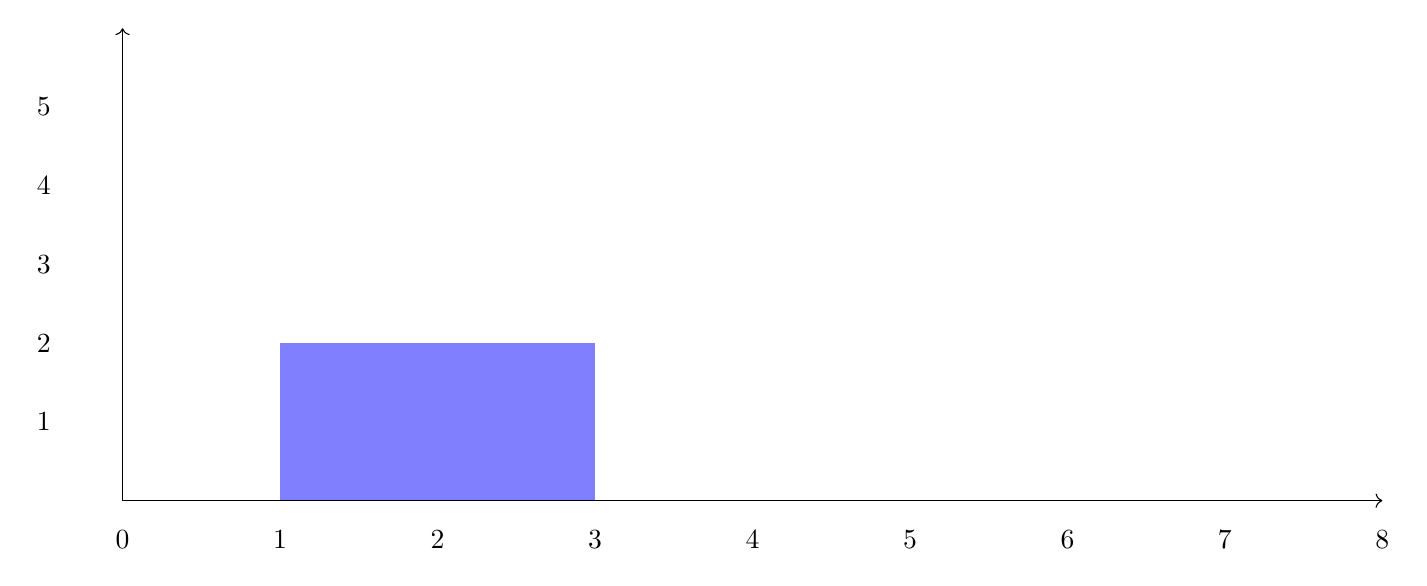
\begin{tikzpicture}
\fill[color=blue!50] (3,0.5cm) rectangle ++(4,2cm);
\draw[->] (1,0.5cm) -- ++(16,0);
\draw[->] (1,0.5cm) -- ++(0,6cm);
\foreach \x / \y in {1/0,3/1,5/2,7/3, 9/4, 11/5, 13/6, 15/7, 17/8}
\node (\x) at (\x, 0) {$\y$};
\foreach \x / \y in {1.5cm/1, 2.5cm/2, 3.5cm/3, 4.5cm/4, 5.5cm/5}
\node (\x) at (0, \x) {$\y$};
\end{tikzpicture}

The maximum height of any square is 2.

After the second drop of positions \lstinline[language=C++, basicstyle=\small\ttfamily, keywordstyle=\bfseries\color{green!40!black}]|[1] = [2, 3]|:
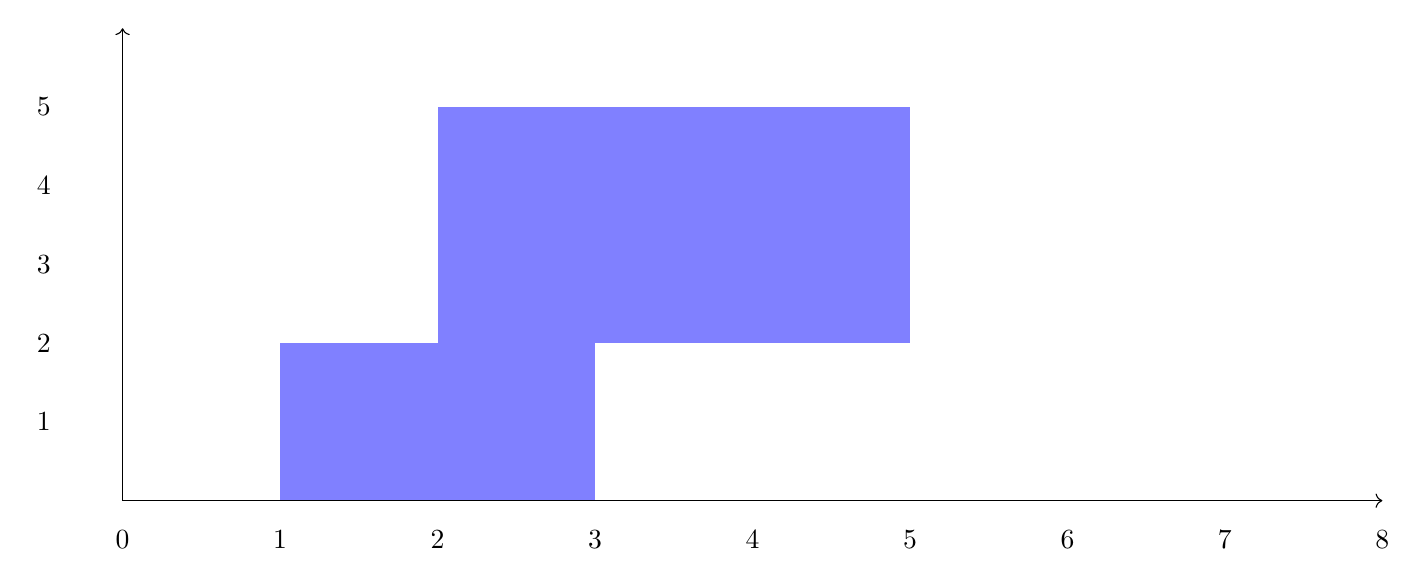
\begin{tikzpicture}
\fill[color=blue!50] (5,2.5cm) rectangle ++(6,3cm);
\fill[color=blue!50] (3,0.5cm) rectangle ++(4,2cm);
\draw[->] (1,0.5cm) -- ++(16,0);
\draw[->] (1,0.5cm) -- ++(0,6cm);
\foreach \x / \y in {1/0,3/1,5/2,7/3, 9/4, 11/5, 13/6, 15/7, 17/8}
\node (\x) at (\x, 0) {$\y$};
\foreach \x / \y in {1.5cm/1, 2.5cm/2, 3.5cm/3, 4.5cm/4, 5.5cm/5}
\node (\x) at (0, \x) {$\y$};
\end{tikzpicture}

The maximum height of any square is 5.  

The larger square stays on top of the smaller square despite where its center of gravity is, because squares are infinitely sticky on their bottom edge.

After the third drop of positions \lstinline[language=C++, basicstyle=\small\ttfamily, keywordstyle=\bfseries\color{green!40!black}]|[1] = [6, 1]|:
\begin{tikzpicture}
\fill[color=blue!50] (13,0.5cm) rectangle ++(2,1cm);
\fill[color=blue!50] (5,2.5cm) rectangle ++(6,3cm);
\fill[color=blue!50] (3,0.5cm) rectangle ++(4,2cm);
\draw[->] (1,0.5cm) -- ++(16,0);
\draw[->] (1,0.5cm) -- ++(0,6cm);
\foreach \x / \y in {1/0,3/1,5/2,7/3, 9/4, 11/5, 13/6, 15/7, 17/8}
\node (\x) at (\x, 0) {$\y$};
\foreach \x / \y in {1.5cm/1, 2.5cm/2, 3.5cm/3, 4.5cm/4, 5.5cm/5}
\node (\x) at (0, \x) {$\y$};
\end{tikzpicture}

The maximum height of any square is still 5.

Thus, we return an answer of \lstinline[language=C++, basicstyle=\small\ttfamily, keywordstyle=\bfseries\color{green!40!black}]|[2, 5, 5]|.
\end{flushleft}

\paragraph{Example 2:}
\begin{flushleft}
\textbf{Input}: \lstinline[language=C++, basicstyle=\small\ttfamily, keywordstyle=\bfseries\color{green!40!black}]|[[100, 100], [200, 100]]|

\textbf{Output}: \lstinline[language=C++, basicstyle=\small\ttfamily, keywordstyle=\bfseries\color{green!40!black}]|[100, 100]|

\textbf{Explanation}: Adjacent squares do not get stuck prematurely - only their bottom edge can stick to surfaces.
\end{flushleft}

\paragraph{Note:}
\begin{itemize}
\item The number of total squares is in range $(1, 1000)$

\item The bottom left of each square is in range $(1,,10^8)$.

\item The side length of each square is  in range $(1,10^6)$.
\end{itemize}

\subsection{Offline Propagation}
Suppose $F[i]$ be the maximum height of the interval specified by \lstinline[language=C++, basicstyle=\small\ttfamily, keywordstyle=\bfseries\color{green!40!black}]|positions[i]|. At the end, we'll return a running max of $F$.

For each square \lstinline[language=C++, basicstyle=\small\ttfamily, keywordstyle=\bfseries\color{green!40!black}]|positions[i]|, the maximum height will get higher by the size of the square we drop. Then, for any future squares that intersect the interval \lstinline[language=C++, basicstyle=\small\ttfamily, keywordstyle=\bfseries\color{green!40!black}]|[left, right)| (where \lstinline[language=C++, basicstyle=\small\ttfamily, keywordstyle=\bfseries\color{green!40!black}]|left = positions[i][0]|, \lstinline[language=C++, basicstyle=\small\ttfamily, keywordstyle=\bfseries\color{green!40!black}]|right = positions[i][0] + positions[i][1]|), we'll update the maximum height of that interval.

\setcounter{lstlisting}{0}
\begin{lstlisting}[style=customc, caption={Offline Propagation}]
vector<int> fallingSquares( vector<vector<int>>& positions )
{
    auto& S = positions;

    //H[i] is the highest
    //height in the range of (S[i][0], S[i][0]+S[i][1])
    vector<int> H( S.size(), 0 );

    for( size_t i = 0; i < S.size(); ++i )
    {
        int range_l = S[i][0];
        int side = S[i][1];
        int range_r = range_l + side;

        //square S[i] is dropped
        //but H[i] does not add its side length
        //thus we need to increment
        //the maximum height in the range
        //of S[i] by the side length.
        H[i] += side;

        for( size_t j = i + 1; j < S.size(); ++j )
        {
            int left = S[j][0];
            int right = S[j][0] + S[j][1];

            if( ( left < range_r ) && ( range_l < right ) )
            {
                //S[j] is overlapped with S[i]
                //we update the maximum length
                //that could be affected by H[i]
                H[j] = ( max )( H[j], H[i] );
            }
        }
    }

    //we need to get
    //the running maximum H
    //as the answer
    vector<int> ans;
    ans.reserve( H.size() );

    int curH = -1;

    for( int h : H )
    {
        curH = ( max )( h, curH );
        ans.push_back( curH );
    }

    return ans;
}
\end{lstlisting}

\subsection{Brute Force with Coordinate Compression}
Since the range left and right ends are limited, we can use a technique called \textbf{coordinate compression} to map these points to adjacent integers. This technique requires a set $S$ and a hash map $M$. Since set can sort the points when inserting, we can get sorted coordinates when iterating through the set $S$.

In this approach, we compress the positions and then for each current square, we first get the maximum height from the range that current square covers, and then update the maximum heights inside this range. To achieve this, we make use of an array $H$ to save maximum height of the interval specified by each square.

\begin{lstlisting}[style=customc, caption={Coordinate Compression}]
vector<int> fallingSquares( vector<vector<int>>& positions )
{
    //compress coordinates
    set<int> coords;

    for( const auto& square : positions )
    {
        coords.insert( square[0] );
        coords.insert( square[0] + square[1] - 1 );
    }

    unordered_map<int, int> m_index;
    int index = 0;

    //map each coord
    //to a continuous integer
    for( int coord : coords )
    {
        m_index.emplace( coord, index++ );
    }

    vector<int> ans;
    ans.reserve( positions.size() );

    vector<int> H( index, 0 );

    int best = 0;

    for( const auto& sq : positions )
    {
        //get the coord index
        int left = m_index[sq[0]];
        int right = m_index[sq[0] + sq[1] - 1];

        //query the maximum height in [left, right]
        int max_h = 0;
        for( int i = left; i <= right; ++i )
        {
            max_h = ( max )( max_h, H[i] );
        }

        //increase the height by the side length
        //of current square
        max_h += sq[1];

        //update maximum height in [left, right]
        for( int i = left; i <= right; ++i )
        {
            H[i] = ( max )( H[i], max_h );
        }

        best = ( max )( best, max_h );
        ans.push_back( best );
    }

    return ans;
}
\end{lstlisting}

\subsection{Segment Tree With Lazy Propagation}
Since we are querying maximum heights in a range, segment tree would be another suitable approach. In this approach, the merge function will get the maximum height from the merged two intervals.

The working flow is same as last approach
\begin{enumerate}
\item Query the maximum height in the range specified by current square.
\item Update the maximum heights in this range.
\item Save running maximum height to the output.
\end{enumerate}

\begin{lstlisting}[style=customc, caption={Segment Tree}]
struct STree
{
    vector<int> tree;
    vector<int> lazy;

    STree( int sz )
        : tree( sz, 0 )
        , lazy( sz, 0 )
    {
    }

    void lazy_prop( int ti, int a_start, int a_end )
    {
        if( lazy[ti] )
        {
            //node tree[ti] has pending updates
            tree[ti] = ( max )( tree[ti], lazy[ti] );

            if( a_start != a_end )
            {
                lazy[2 * ti + 1] = ( max )( lazy[2 * ti + 1], lazy[ti] );
                lazy[2 * ti + 2] = ( max )( lazy[2 * ti + 2], lazy[ti] );
            }

            lazy[ti] = 0;
        }
    }

    bool check_range( int a_start, int a_end, int q_start, int q_end )
    {
        if( a_start > a_end )
        {
            return false;
        }

        if( ( a_start > q_end ) || ( a_end < q_start ) )
        {
            //cover range [a_start, a_end] does not
            //overlap with query range [q_start, q_end]
            return false;
        }

        return true;
    }

    bool is_inside_query( int a_start, int a_end, int q_start, int q_end )
    {
        if( ( a_start >= q_start ) && ( a_end <= q_end ) )
        {
            //cover range [a_start, a_end] is completely inside
            //query range [q_start, q_end]
            return true;
        }

        return false;
    }

    int query( int ti, int a_start, int a_end, int q_start, int q_end )
    {
        lazy_prop( ti, a_start, a_end );

        if( !check_range( a_start, a_end, q_start, q_end ) )
        {
            //either invalid cover range
            //or not overlap with query range
            return 0;
        }

        if( is_inside_query( a_start, a_end, q_start, q_end ) )
        {
            //cover range is completely inside query range
            return tree[ti];
        }

        //cover range is overlapped with query range
        int mid = ( a_start + a_end ) / 2;

        //left result
        int res_l = query( 2 * ti + 1, a_start, mid, q_start, q_end );
        //right result
        int res_r = query( 2 * ti + 2, mid + 1, a_end, q_start, q_end );

        return ( max )( res_l, res_r );
    }

    void update( int ti, int a_start, int a_end, int q_start, int q_end, int value )
    {
        lazy_prop( ti, a_start, a_end );

        if( !check_range( a_start, a_end, q_start, q_end ) )
        {
            //either invalid cover range
            //or not overlap with query range
            return;
        }

        if( is_inside_query( a_start, a_end, q_start, q_end ) )
        {
            //cover range is completely inside query range
            tree[ti] = ( max )( tree[ti], value );

            //put impending update to lazy array
            if( a_start != a_end )
            {
                lazy[2 * ti + 1] = ( max )( lazy[2 * ti + 1], value );
                lazy[2 * ti + 2] = ( max )( lazy[2 * ti + 2], value );
            }
        }
        else
        {
            int mid = ( a_start + a_end ) / 2;
            //update left
            update( 2 * ti + 1, a_start, mid, q_start, q_end, value );
            //update right
            update( 2 * ti + 2, mid + 1, a_end, q_start, q_end, value );

            //update current node
            tree[ti] = ( max )( tree[2 * ti + 1], tree[2 * ti + 2] );
        }
    }
};


vector<int> fallingSquares( vector<vector<int>>& positions )
{

    //coordinat compression
    set<int> coords;

    for( const auto& p : positions )
    {
        coords.insert( p[0] );
        coords.insert( p[0] + p[1] - 1 );
    }

    unordered_map<int, int> m_index;

    int N = 0;

    for( int coord : coords )
    {
        m_index.emplace( coord, N++ );
    }

    int h_tree = 1;

    while( ( 1 << h_tree ) < N )
    {
        ++h_tree;
    }

    int tree_size = ( 1 << h_tree ) * 2;


    //create segement tree
    STree stree( tree_size );


    int best = 0;
    vector<int> ans( positions.size() );

    int i_ans = 0;

    for( const auto& p : positions )
    {
        int left = m_index[p[0]];
        int right = m_index[p[0] + p[1] - 1];

        //the query is starting from the root
        //ti=0, and cover range is [0, N-1]
        int h = stree.query( 0, 0, N - 1, left, right );
        //increase h by current square side length
        h += p[1];

        //update in range [left, right]
        //starting from the root ti=0, and cover range
        //is [0, N-1]
        stree.update( 0, 0, N - 1, left, right, h );

        best = ( max )( best, h );

        ans[i_ans++] = best;
    }

    return ans;
}
\end{lstlisting}
\end{document}
